\documentclass[12pt,chapterheads]{ucsd}

% package setup
\usepackage[colorlinks=false,linkcolor=black,urlcolor=black,bookmarksopen=true]{hyperref}
\usepackage{bookmark}
\usepackage{amsmath, amscd, amssymb, amsthm, xfrac}
\usepackage{scrextend}
\usepackage{pslatex}
\usepackage{graphicx}
\makeatletter
\gdef\@ptsize{2}% 12pt documents
\let\@currsize\normalsize
\makeatother
\usepackage{setspace}
\doublespace
\usepackage[font=small, width=0.9\textwidth]{caption}
\usepackage[T1]{fontenc}
\usepackage{mathptmx}
\usepackage{url}
\urlstyle{same}
\usepackage{microtype}
\usepackage{footnote}
\makesavenoteenv{tabular}
\makesavenoteenv{table}
\usepackage{rotating}
\usepackage{array}
\usepackage{booktabs}
\newcolumntype{P}[1]{>{\centering\arraybackslash}m{#1}}
\usepackage[acronym]{glossaries}

%%% PYTHON HIGHLIGHTING
\DeclareFixedFont{\ttb}{T1}{txtt}{bx}{n}{8} % for bold
\DeclareFixedFont{\ttm}{T1}{txtt}{m}{n}{8}  % for normal
% Custom colors
\usepackage{color}
\definecolor{deepblue}{rgb}{0,0,0.5}
\definecolor{deepred}{rgb}{0.6,0,0}
\definecolor{deepgreen}{rgb}{0,0.5,0}
\usepackage{listings}
% Python style for highlighting
\newcommand\pythonstyle{\lstset{
language=Python,
basicstyle=\ttm,
otherkeywords={self},             % Add keywords here
keywordstyle=\ttb\color{deepblue},
emph={MyClass,__init__},          % Custom highlighting
emphstyle=\ttb\color{deepred},    % Custom highlighting style
stringstyle=\color{deepgreen},
frame=tb,                         % Any extra options here
showstringspaces=false            % 
}}
% Python environment
\lstnewenvironment{python}[1][]
{
\pythonstyle
\lstset{#1}
}
{}
% Python for external files
\newcommand\pythonexternal[2][]{{
\pythonstyle
\lstinputlisting[#1]{#2}}}
% Python for inline
\newcommand\pythoninline[1]{{\pythonstyle\lstinline!#1!}}

%% define section names
\newcommand{\abbrevtitle}{List of Abbreviations}
\newcommand{\dualbirthtitle}{A Two-State Model of Tree Evolution and its Applications to \textit{Alu} Retrotransposition}
\newcommand{\educationtitle}{Bioinformatics Education}
\newcommand{\favitestitle}{FAVITES: Simultaneous Simulation of Transmission Networks, Phylogenetic Trees, and Sequences}
\newcommand{\introtitle}{Introduction}
\newcommand{\proacttitle}{ProACT: Prioritization Using Ancestral Edge Lengths}
\newcommand{\treeswifttitle}{TreeSwift: A Massively Scalable Python Tree Package}

%% define other useful commands
\newcommand{\bigO}{\textrm{O}}

%% define acronyms
\newacronym{API}{API}{Application Program Interface}
\newacronym{ART}{ART}{Antiretroviral Therapy}
\newacronym{BA}{BA}{Barab\'asi--Albert}
\newacronym{BF}{BF}{Blum and Fran\c{c}ois~(2006)}
\newacronym{bp}{bp}{base pairs}
\newacronym{CHRP}{CHRP}{California HIV/AIDS Research Program}
\newacronym{CMA}{CMA}{Cumulative Moving Average}
\newacronym{DAG}{DAG}{Directed Acyclic Graph}
\newacronym{DNA}{DNA}{Deoxyribonucleic Acid}
\newacronym{EPU}{EPU}{Extended Polya Urn}
\newacronym{ER}{ER}{Erd\H os--R\'enyi}
\newacronym{F81}{F81}{Felsenstein~(1981)}
\newacronym{GTR}{GTR}{General Time-Reversible}
\newacronym{HIV}{HIV}{Human Immunodeficiency Virus}
\newacronym{HKY85}{HKY85}{Hasegawa, Kishino, and Yano~(1985)}
\newacronym{HMM}{HMM}{Hidden Markov Model}
\newacronym{ITS}{ITS}{Intelligent Tutor System}
\newacronym{JC69}{JC69}{Jukes and Cantor~(1969)}
\newacronym{JSD}{JSD}{Jensen--Shannon Divergence}
\newacronym{K80}{K80}{Kimura~(1980)}
\newacronym{KS}{KS}{Kirkpatrick and Slatkin~(1993)}
\newacronym{LANL}{LANL}{Los Alamos National Laboratory}
\newacronym{LTT}{LTT}{Lineages Through Time}
\newacronym{MAIT}{MAIT}{Massive Adaptive Interactive Text}
\newacronym{MCMC}{MCMC}{Markov Chain Monte Carlo}
\newacronym{ML}{ML}{Maximum-Likelihood}
\newacronym{MOOC}{MOOC}{Massive Open Online Course}
\newacronym{MS}{MS}{Matching Split}
\newacronym{MSA}{MSA}{Multiple Sequence Alignment}
\newacronym{NGS}{NGS}{Next Generation Sequencing}
\newacronym{PDF}{PDF}{Probability Density Function}
\newacronym{PIRC}{PIRC}{Primary Infection Resource Consortium}
\newacronym{PLH}{H$^+$I}{HIV-Positive Individual}
\newacronym{PLWH}{SH$^+$I}{Sampled HIV-Positive Individual}
\newacronym{pol}{\textit{pol}}{Polymerase}
\newacronym{POSET}{POSET}{Partially Ordered Set}
\newacronym{PrEP}{PrEP}{Pre-Exposure Prophylaxis}
\newacronym{QALY}{QALY}{Quality-Adjusted Life-Year}
\newacronym{RF}{RF}{Robinson--Foulds}
\newacronym{RNA}{RNA}{Ribonucleic Acid}
\newacronym{SINE}{SINE}{Short Interspersed Nuclear Element}
\newacronym{SSA}{SSA}{Simple Sampling Algorithm}
\newacronym{TN93}{TN93}{Tamura and Nei~(1993)}
\newacronym{tMRCA}{tMRCA}{Time of the Most Recent Common Ancestor}
\newacronym{UNAIDS}{UNAIDS}{the Joint United Nations Programme on HIV/AIDS}
\newacronym{WES}{WES}{Whole Exome Sequencing}
\newacronym{WGS}{WGS}{Whole Genome Sequencing}
\newacronym{WS}{WS}{Watts--Strogatz}
\makeglossaries

\begin{document}

%% include sections
%% Dissertation Info
\title{Mathematical Modeling of Viral Evolution and Epidemiology}
\author{Alexander Niema Moshiri}
\degreeyear{2019}
\degreetitle{Doctor of Philosophy}
\field{Bioinformatics and Systems Biology}
%\specialization{Anthropogeny}  % If you have a specialization, add it here

%% Committee Info
\chair{Professor Siavash Mirarab}
\cochair{Professor Pavel A. Pevzner}
\othermembers{
Professor Vineet Bafna\\
Professor David M. Smith\\
Professor Joel O. Wertheim\\
}
\numberofmembers{5} % |chair| + |cochair| + |othermembers|

%% Define Acknowledgement Statements (to avoid typos when copying)
\newcommand{\ackfavites}{Chapter~\ref{chap:favites}, in full, is a reprint of the material as it appears in ``\favitestitle'' (2018). Moshiri, Niema; Ragonnet-Cronin, Manon; Wertheim, Joel; Mirarab, Siavash, \textit{Bioinformatics}, bty921. The dissertation author was the primary investigator and first author of this paper.}
\newcommand{\ackdualbirth}{Chapter~\ref{chap:dualbirth}, in full, is a reprint of the material as it appears in ``\dualbirthtitle'' (2017). Moshiri, Niema; Mirarab, Siavash, \textit{Systematic Biology}, 67(3), 475-489. The dissertation author was the primary investigator and first author of this paper.}
\newcommand{\ackproact}{Chapter~\ref{chap:proact}, in full, has been submitted for publication of the material as it may appear in ``\proacttitle'' (2019) Moshiri, Niema; Smith, Davey; Mirarab, Siavash, \textit{Molecular Biology and Evolution}. The dissertation author was the primary investigator and first author of this paper.}
\newcommand{\acktreeswift}{Chapter~\ref{chap:treeswift}, in full, has been submitted for publication of the material as it may appear in ``\treeswifttitle'' (2019) Moshiri, Niema, \textit{SoftwareX}. The dissertation author was the primary investigator and sole author of this paper.}

%% START FRONTMATTER
\begin{frontmatter}
\makefrontmatter

%% Dedication
\begin{dedication}
\vspace*{\fill}
I dedicate this dissertation to Ladan Moshiri, Ramin Moshiri, and Michelle Roxanna Moshiri-Warncke for years of love and support.
~\\~\\~\\
I dedicate this dissertation to Karen George for always being by my side.
~\\~\\~\\
I dedicate this dissertation to Ryan Micallef and Felix Garcia for teaching me to live my life a quarter mile at a time.
~\\~\\~\\
I dedicate this dissertation to all my friends in the Bioinformatics and Systems Biology program for some of the best memories of my life.
\vspace*{\fill}
\end{dedication}

%% Epigraph
\begin{epigraph}
\begin{center}
\begin{minipage}{0.65\linewidth}
\onehalfspacing
{\large
\textit{Folk in these stories had lots of chances of turning back, only they didn't. Because they were holding onto something.}\\
~\\
\textit{What are we holding onto, Sam?}\\
~\\
\textit{That there's some good in this world, Mr. Frodo. And it's worth fighting for.}
\begin{flushright}
---J.R.R. Tolkien
\end{flushright}
}
\end{minipage}
\end{center}
\end{epigraph}

%% Table of Contents
\tableofcontents

%% List of Abbreviations
\newpage
\addcontentsline{toc}{chapter}{\abbrevtitle}
\begin{center}\expandafter\MakeUppercase\expandafter{\abbrevtitle}\end{center}
\let\clearpage\relax
\vspace*{-2cm}
\printglossary[type=\acronymtype,title={}]

%% List of Symbols

%% List of Figures and Tables
\listoffigures
\listoftables


%% Acknowledgements
\begin{acknowledgements}
I would like to thank all of the people who have helped me throughout my Ph.D. My colleagues in the Bioinformatics and Systems Biology Graduate Program and in the Computer Science and Engineering department have been great to work with, especially Jens Luebeck, Margaret Donovan, Bill Greenwald, Ben Pullman, and Argus Athanas. I enjoyed having the support of such excellent lab mates as Erfan Sayyari, Metin Balaban, Uyen Mai, Maryam Rabiee, Sina Malekian, and Chao Zhang.
I would also like to thank Prof.~Joel Wertheim, Manon Ragonnet-Cronin, Prof.~Davey Smith, and Prof.~Sanjay Mehta for teaching so much about the molecular biology and epidemiology of HIV.
I am truly blessed to have been able to work with such amazing people.

I would not be where I am today (both figuratively and literally) without the mentorship of Prof.~Vineet Bafna. I met him early on in my undergraduate career, and he has been the source of sage wisdom throughout my entire academic career thus far. It was largely because of him that I decided to continue to pursue graduate education in Bioinformatics, and I am thankful that his guidance led me down this path.

I am grateful of Prof.~Pavel Pevzner for taking me under his wing at a time when I was somewhat lost regarding my career aspirations. Growing up, I always thought I wanted to become a medical doctor, but I always had a strong passion for technology. It was under his mentorship that I recognized the possibility to merge these two seemingly unrelated fields, and I was able to see the biomedical applications of Computer Science. He also introduced me to the field of Bioinformatics Education, and it was because of his guidance that I realized my passion for teaching, and I am honored he took a chance on me. He is truly a visionary, and I am happy to have been able to work with him.

When starting a Ph.D. program, one of the most stressful thoughts is ``Will I find a good mentor?'', and I was extremely fortunate to have found Prof.~Siavash Mirarab. I cannot thank him enough for all the time and effort he has taken to make my Ph.D. experience productive and intellectually stimulating. From the long sessions in which we'd be working on an algorithmic problem together, to the hours he would spend helping me revise my manuscripts, the effort he took to mentor me has instilled within me far more than I could have imagined. I aspire to be as brilliant of a scientist as he one day, and I hope to be as great of a mentor as he was to me.

\ackfavites

\ackdualbirth

\ackproact

\acktreeswift
\end{acknowledgements}

%% Vita
\begin{vitapage}
\begin{vita}
\item[2015] B.~S. in Bioengineering: Bioinformatics, University of California, San Diego
\item[2015-2016] Teaching Assistant, University of California, San Diego
\item[2017] Associate Instructor, University of California, San Diego
\item[2015-2019] Research Assistant, University of California, San Diego
\item[2019] Ph.~D. in Bioinformatics and Systems Biology, University of California, San Diego
\end{vita}
\begin{publications}
\item \textbf{Niema Moshiri} (2019). ``Why Do I Look Like My Mom and Dad? Plants and Animals Inherit Traits From Parents,'' \textit{STEMTaught}
\item Metin Balaban, \textbf{Niema Moshiri}, Uyen Mai, and Siavash Mirarab (2019). ``TreeCluster: Clustering Biological Sequences using Phylogenetic Trees,'' \textit{GLBIO 2019}, doi:~10.1101/591388
\item Adam Rule, Amanda Birmingham, Cristal Zuniga, Ilkay Altintas, Shih-Cheng Huang, Rob Knight, \textbf{Niema Moshiri}, Mai H. Nguyen, Sara Brin Rosenthal, Fernando Pérez, and Peter W. Rose (2019). ``Ten Simple Rules for Reproducible Research in Jupyter Notebooks,'' \textit{PLOS Computational Biology (in press)}, arXiv:~1810.08055
\item \textbf{Niema Moshiri} and Liz Izhikevich (2018). \textit{Design and Analysis of Data Structures}, Amazon KDP, ISBN:~1981017232
\item \textbf{Niema Moshiri}, Manon Ragonnet-Cronin, Joel O. Wertheim, and Siavash Mirarab (2018). ``FAVITES: simultaneous simulation of transmission networks, phylogenetic trees, and sequences,'' \textit{Bioinformatics}, doi:~10.1093/bioinformatics/bty921
%\item \textbf{Niema Moshiri} (2018). ``The dual-Barab\'asi-Albert model,'' \textit{arXiv}, arXiv:~1810.1810.10538
%\item \textbf{Niema Moshiri} (2018). ``TreeN93: a non-parametric distance-based method for inferring viral transmission clusters,'' \textit{bioRxiv}, doi:~10.1101/383190
\item \textbf{Niema Moshiri} (2018). ``TreeSwift: a massively scalable Python tree package,'' \textit{bioRxiv}, doi:~10.1101/325522
\item \textbf{Niema Moshiri}, Liz Izhikevich, and Christine Alvarado (2018). ``Data Structures: An Active Learning Approach,'' \textit{edX}
\item \textbf{Niema Moshiri}, Phillip Compeau, and Pavel Pevzner (2017). ``Analyze Your Genome!,'' \textit{edX}
\item Phillip Compeau, \textbf{Niema Moshiri}, and Pavel Pevzner (2017). ``Introduction to Genomic Data Science,'' \textit{edX}
%\item \textbf{Niema Moshiri} (2017). ``A linear-time algorithm to sample the dual-birth model,'' \textit{bioRxiv}, doi:~10.1101/226423
\item \textbf{Niema Moshiri} and Siavash Mirarab (2017). ``A Two-State Model of Tree Evolution and Its Applications to Alu Retrotransposition,'' \textit{Systematic Biology}, 67(3), 475-489. doi:~10.1093/sysbio/syx088
\end{publications}
\end{vitapage}

%% Abstract
\begin{abstract}
Phylogenetic trees can be used to study the evolution of any sequence that evolves, including viruses. In a viral epidemic, the history of transmission events defines constraints on the evolutionary history of the viral population. Models of tree evolution describe probability distributions over the space of tree shapes and can be used to simulate trees that capture the evolutionary patterns of real world phenomena as well as to infer evolutionary parameters inherently of interest to the biologist. The spread of many viruses is driven by social and sexual networks, and because of the relationship between their evolutionary and transmission histories, phylogenetic inference from viral sequences can be used to improve the inference of patterns of the epidemic, which in turn can greatly enhance epidemiological intervention. The simultaneous simulation of viral transmission network, phylogenetic tree, and sequences can provide a method to observe the effects of virus model parameters on the epidemic as well as to study the accuracies and errors of transmission inference tools. Further, the development of massively-scalable tools to analyze ultra-large datasets of viral sequences can aid epidemiologists in the real-time surveillance of the spread of disease. In an effort to contribute to these ideas, I developed a novel framework to simulate viral transmission networks, phylogenetic trees, and sequences, developed a novel evolutionary model, studied the effects of model parameters on epidemic outcomes via simulation experiments using the proposed framework, developed a scalable and non-parametric method of transmission risk prioritization, and contributed to publicly-accessible Bioinformatics education.
\end{abstract}
\end{frontmatter}

%% END FRONT MATTER
%%% START INTRO CHAPTER
\addcontentsline{toc}{chapter}{\introtitle}
\chapter*{\introtitle}
\clearpage

Although they are typically associated with the study of the evolution of species, phylogenetic trees can be used to study the evolution of any sequence that evolves. For example, phylogenetic methods have been used to study the evolution of multicopy gene families~ \cite{Page1997}, cancer genomes~\cite{El-Kebir2016,Nowell1976}, antibodies~\cite{Litman1993,Robinson2015,Safonova2015}, segmental duplicates~\cite{Bailey2006,Jiang2007}, and transposable genomic elements~\cite{Dewannieux2003,Moshiri2017}, which are all entities that evolve \textit{within} the genome of a single species. Further, they can be used to study the evolution of viruses, both within and across hosts~\cite{Frost2001,Lemey2006,Vrancken2014}. In the case of viruses, the history of transmission events constrains the evolutionary history, such as imposing a bottleneck at the time of each transmission~\cite{Carlson2014}.

The spread of many infectious diseases is driven by social and sexual networks~\cite{Rivas2012}, and reconstruction of their transmission histories from molecular data can greatly enhance intervention. For example, network-based statistics for measuring \gls{HIV} treatment effects can yield increased statistical power~\cite{Wertheim2011}; the analysis of the growth of \gls{HIV} infection clusters can yield actionable epidemiological information for disease treatment and prevention~\cite{Aldous2012,Brenner2013}; transmission-aware models can be used to infer rates of \gls{HIV} evolution~\cite{Vrancken2014}. The ability to infer properties and patterns of the transmission history of a viral epidemic allows public health officials to intervene and attempt to prevent the spread of the virus. In the case of \gls{HIV}, patients who adhere to \gls{ART} can become ``virally suppressed,'' meaning the virus is kept at bay, resulting in slower progression of the \gls{HIV} disease as well as a significant reduction in transmission risk~\cite{AIDSinfo2019}. Thus, the ability to predict which individuals are most at-risk of transmitting the virus would provide public health officials actionable information: they can take measures to ensure high-risk individuals are able to continuously adhere to \gls{ART}.

The ability to infer and reconstruct properties of a transmission network has been researched extensively in recent years~\cite{Wertheim2017,Ragonnet-Cronin2019}, and many tools exist that attempt to use molecular data to try to perform this inference~\cite{Rose2017}. For example, PhyloPart~\cite{Prosperi2011}, Cluster Picker~\cite{Ragonnet-Cronin2013}, and TreeCluster~\cite{Balaban2019} infer transmission clusters using phylogenies inferred from viral sequences. HIV-TRACE, on the other hand, infers transmission clusters directly from sequences~\cite{Pond2018}. While these tools have been used to analyze real datasets~\cite{Campbell2017}, the accuracies, errors, and limitations of these methods are still poorly understood.

By utilizing models of social contact networks, viral transmission, tree evolution, and sequence evolution together, epidemiologists can define complex probabilistic distributions composed of sub-models. These complex distributions can be sampled to simulate data representative of a virus of interest as it spreads through a population of interest, and the resulting data can be used to evaluate the accuracies of transmission network inference methods as well as to study trends and patterns of an epidemic as a function of the various model parameters to gain insights into the mechanisms driving the epidemic of interest~\cite{Ratmann2017}. However, many existing tools to perform such epidemic simulations have model assumptions that the user cannot relax or change. In Chapter~\ref{chap:favites}, I will discuss FAVITES: a novel epidemic simulation framework I developed that provides flexibility in terms of the model assumptions about the epidemic, allowing the user to control the generative model in minute detail. The framework is defined by a series of interactions of abstract modules, and each \textit{implementation} of a module defines the model assumptions. Thus, users are free to select whichever module implementations (and thus model assumptions) that best fit their epidemic of interest. In addition to presenting the tool, I will describe in detail a simulation experiment designed to emulate the San Diego \gls{HIV} epidemic between 2005 and 2014, and I will use the simulated data to compare and contrast existing transmission clustering methods.

Of course, the ability to simulate an epidemic depends entirely on the existence of statistical models that appropriately describe the processes of the epidemic of interest. Models of tree evolution describe probability distributions over the space of tree shapes~\cite{Yule1925,Aldous2001}, which can be used as the prior distribution in a Bayesian inference~\cite{Drummond2007,Mooers2012,Sayyari2016}, to generate null distributions describing certain neutral processes~\cite{Guyer1991,Kirkpatrick1993,Agapow2002}, or to infer evolutionary parameters inherently of interest to the biologist~\cite{Morlon2014}. Similarly, generalized epidemic models describe probability distributions over the space of transmission networks~\cite{Sahneh2013}, and simulations that sample the distributions defined by these stochastic models allows epidemiologists to study infection patterns of disease epidemics~\cite{Sahneh2017}. Further, network models describe probability distributions over graphs, and they can be used to capture features of networks of interactions (e.g. social interactions between humans)~\cite{Watts1998,Watts1999,Barabasi1999,Erdos1959}. Lastly, models of sequence evolution describe the mutation of a sequence over time~\cite{Jukes1969,Kimura1980,Felsenstein1981,Tamura1993,Tavare1986}, and they can be used to simulate the evolution of a sequence down a phylogeny~\cite{Rambaut1997} as well as to infer the evolutionary history of a set of sequences~\cite{Felsenstein2003}. In the case of retroviruses and retrotransposons, which replicate via reverse transcription~\cite{Whitcomb1992} and may undergo significant selection pressure~\cite{Wood2009}, a neutral model of tree evolution like the Yule~\cite{Yule1925} or Coalescent~\cite{Kingman1982} may not be appropriate. In Chapter~\ref{chap:dualbirth}, I will discuss the dual-birth model, a novel model of tree evolution that is motivated by the retrotransposition of \textit{Alu} elements in the human genome~\cite{Batzer2002}. I will derive various probabilistic distributions and theoretical expectations of trees sampled under the model, and I will then present two approaches for estimating model parameters from a given phylogeny. I will then present the results of an analysis of close to one million \textit{Alu} sequences from the human genome in which I infer the dual-birth model parameters and present an estimate of the number of active \textit{Alu} elements, a topic of much debate~\cite{Price2004,Deininger2011,Cordaux2004}.

The goal of many transmission clustering analyses is to learn about the dynamics of a virus through a given population, often to try to predict which sub-populations may be spreading the virus more rapidly~\cite{Wertheim2011,Wertheim2017,Little2014}. However, transmission clustering is essentially a way of summarizing the relationships between the sampled viral sequences, and instead of performing predictions and inferences on these summaries, what if we were able to infer properties of interest directly from the evolutionary relationships of the viruses? In Chapter~\ref{chap:proact}, I investigate a single specific question: Given a set of viral sequences sampled from people living with \gls{HIV}, can I predict which individuals are most at-risk of transmitting the virus in the future? In an attempt to address this question, I present ProACT, a tool that attempts to prioritize people living with \gls{HIV} based on risk of future transmissions. ProACT depends only on the viral phylogeny and does not require any demographic information from the patients, meaning it is not sensitive to error-prone survey data, and most importantly, it is less prone to bias.

A primary focus of mine is the ability to execute phylogenetic methods like ProACT in a massively-scalable fashion. The scalability of a computational tool is primarily dependant on two things: (1) the theoretical time complexity of the algorithm, and (2) the efficiency of the implementation of the algorithm. While developing FAVITES and ProACT, I found that, although the phylogenetic algorithms I designed were quite fast in theory, my implementations using existing tree-manipulation packages were much slower than I anticipated due to significant overhead in loading and initializing my ultra-large phylogenies. In Chapter~\ref{chap:treeswift}, I will present TreeSwift, a new Python package for traversing and manipulating trees. I will describe its implementation design, demonstrate some of its features, and compare its execution time for various common tree algorithms against existing packages.

As can be seen, as the cost of sequencing decreases, the amount of viral sequence data available to researchers is growing rapidly, and as a result, the field of Epidemiology is becoming increasingly dependent on scalable computational methods. However, many researchers in the fields of Epidemiology and Molecular Biology have never received formal education in computation. In recent years, computational courses have started appearing in undergraduate Biology major curricula, and while this will provide computational skills to the next generation of biomedical and epidemiological researchers, it does not benefit the current generation of professionals. In Chapter~\ref{chap:education}, I will present my contributions to Bioinformatics education in the form of developing novel \glspl{MOOC} and \glspl{MAIT}, and I will discuss the pedagogical philosophy I employed in developing my learning materials.

In summary, I show that modern studies in viral epidemiology require the ability to perform simulation experiments that can appropriately capture the virus and population of interest, which thus requires tools to run such simulations efficiently as well as statistical models that make realistic assumptions. I also show that the ability to infer actionable epidemiological information from molecular data is an open problem. In this dissertation, I present a novel framework for epidemic simulations, provide a novel model of phylogenetic evolution (and derive probabilistic distributions and theoretical expectations of trees sampled under the model), demonstrate the effectiveness of a novel phylogenetic tool for prioritizing people living with \gls{HIV} based on their risk of future transmissions, and introduce a novel package for performing tree traversals and manipulations efficiently on ultra-large phylogenies. I also discuss my contributions to Bioinformatics education.

%% END INTRO CHAPTER
%% START FAVITES CHAPTER
\chapter{\favitestitle}
\label{chap:favites}
\newpage

\textit{Motivation} --- The ability to simulate epidemics as a function of model parameters allows insights that are unobtainable from real datasets. Further, reconstructing transmission networks for fast-evolving viruses like \gls{hiv} may have the potential to greatly enhance epidemic intervention, but transmission network reconstruction methods have been inadequately studied, largely because it is difficult to obtain ``truth'' sets on which to test them and properly measure their performance.

\textit{Results} --- We introduce FAVITES, a robust framework for simulating realistic datasets for epidemics that are caused by fast-evolving pathogens like \gls{hiv}. FAVITES creates a generative model to produce contact networks, transmission networks, phylogenetic trees, and sequence datasets, and to add error to the data. FAVITES is designed to be extensible by dividing the generative model into modules, each of which is expressed as a fixed API that can be implemented using various models. We use FAVITES to simulate \gls{hiv} datasets and study the realism of the simulated datasets. We then use the simulated data to study the impact of the increased treatment efforts on epidemiological outcomes. We also study two transmission network reconstruction methods and their effectiveness in detecting fast-growing clusters.

\textit{Availability and implementation} --- FAVITES is available at \url{https://github.com/niemasd/FAVITES}, and a Docker image  can be found on DockerHub (\url{https://hub.docker.com/r/niemasd/favites}).

\section{Introduction}
The spread of many infectious diseases is driven by social and sexual networks~\cite{Kelly1991}, and reconstructing their transmission histories from molecular data may be able to enhance intervention. For example, network-based statistics for measuring the effects of \gls{art} in \gls{hiv} can yield increased statistical power~\cite{Wertheim2011}; the analysis of the growth of HIV infection clusters can yield actionable epidemiological information for disease control~\cite{Lewis2008}; transmission-aware models can be used to infer HIV evolutionary rates~\cite{Vrancken2014}.

%% END FAVITES CHAPTER
\newcommand{\BL}{D}
\newcommand{\CH}[1]{c(#1)}
\newcommand{\LB}[1]{l_{#1}}
\newcommand{\LBh}{n_l}
\newcommand{\NV}{N}
\newcommand{\RBh}{n_r}
\newcommand{\RN}{\psi}
\newcommand{\RNALL}{\Psi}
\newcommand{\SD}{\omega}
\newcommand{\SDALL}{\Omega}
\newcommand{\TBL}{L}
\newcommand{\TO}{T^\SD}
\newcommand{\TR}{T^\RN}
\newcommand{\TRO}{\TR_{\SD}}
\newcommand{\bl}{\delta}
\newcommand{\child}[2]{#1_{#2}}
\newcommand{\defeq}{=}
\newcommand{\la}{\lambda_a}
\newcommand{\lb}{\lambda_b}
\newcommand{\li}{\lambda_i}
\newcommand{\leaf}{\otimes}
\newcommand{\tav}{\tau'}
\newcommand{\tO}{t^\SD}

\newtheorem{conjecture}{Conjecture}
\newtheorem{corollary}{Corollary}
\newtheorem{lemma}{Lemma}
\newtheorem{theorem}{Theorem}

%% START DUAL-BIRTH CHAPTER
\chapter{\dualbirthtitle}
\label{chap:dualbirth}
\clearpage

Models of tree evolution have mostly focused on capturing the cladogenesis processes behind speciation. Processes that derive the evolution of genomic elements, such as repeats, are not necessarily captured by these existing models. In this paper, we design a model of tree evolution that we call the dual-birth model, and we show how it can be useful in studying the evolution of short \textit{Alu} repeats found in the human genome in abundance. The dual-birth model extends the traditional birth-only model to have two rates of propagation, one for active nodes that propagate often, and another for inactive nodes, that with a lower rate, activate and start propagating. Adjusting the ratio of the rates controls the expected tree balance. We present several theoretical results under the dual-birth model, introduce parameter estimation techniques, and study the properties of the model in simulations. We then use the dual-birth model to estimate the number of active \textit{Alu} elements and their rates of propagation and activation in the human genome based on a large phylogenetic tree that we build from close to one million \textit{Alu} sequences.

\section{Introduction}
Phylogenetic trees can be used to study the evolution of not just species, but of any sequence that evolves. For example, multi-copy gene families~\cite{Page1997,Finn2014}, cancer genomes~\cite{Nowell1976,El-Kebir2016}, antibodies~\cite{Litman1993,Robinson2015,Safonova2015}, segmental duplicates~\cite{Bailey2006,Jiang2007}, and long or short interspersed nuclear elements~\cite{Dewannieux2003} are all biological sequences that evolve, and many of these evolve \textit{within} the genome of a single species. The process of diversification for many evolving entities can be characterized by propagation: an original copy of a sequence creates a new copy, and the two copies evolve independently by accumulating mutations. Phylogenetics provides a natural framework for studying such processes, but several challenges present themselves.

Given sufficiently long sequences and assuming our models of sequence evolution are reasonably accurate, we can recover the phylogenetic trees from sequence data with high accuracy~ \cite{Felsenstein2003,Roch2010}. However, unlike species-tree reconstruction, in which the entire genome can be used, reconstructing phylogenies of gene families, repeats, or antibodies is limited by the length of the evolving entity. As a result, high levels of uncertainty are to be expected in trees reconstructed from these types of sequences. These inherent limitations make accurate modeling of underlying processes crucial, perhaps even more so than species-tree reconstruction.

Models of tree evolution describe probability distributions over the space of tree shapes ~\cite{Yule1925,Brown1994,Aldous2001} and are useful in several ways. They can be used as the prior distribution in a Bayesian inference~\cite{Drummond2007,Mooers2012,Sayyari2016}. They can also generate null distributions describing certain neutral evolutionary process, which may then be rejected by trees inferred from the data~\cite{Guyer1991,Kirkpatrick1993,Agapow2002}. Moreover, the diversification parameters are inherently of interest to the biologist~\cite{Morlon2014}. Two well-known models of tree evolution are Yule (birth-only), in which each branch splits by a Poisson process with a constant rate, and birth-death, in which, in addition to birth, branches can go extinct with a constant rate. Each of these models have limitations and have inspired the development of several alternative models~\cite{Aldous1996,Steel2001,Ford2005,Blum2006,Jones2011,Maddison2007}.

A main feature of a tree evolution model is the expected tree shape, especially the tree balance (Fig.~\ref{fig:dualbirth-model}). The Yule model generates relatively balanced trees~\cite{McKenzie2000}, more so than typically seen in phylogenetic trees~\cite{Blum2006}. Some systems, such as certain viruses, are especially known to have very unbalanced trees~\cite{Volz2013}. Most models of evolution are exchangeable, meaning that, after a split, the two branches are indistinguishable. When evolution works in a series of propagation events (i.e., where an element copies itself), there is a natural way in which one of the child branches corresponds to the parent branch~\cite{Lambert2013}. The new copy may have properties that are different from the original branch, and as a result, non-exchangeable models may be more appropriate. For example, the new child may be initially incapable of propagation until it \textit{activates}. In such situations, the tree will tend to be unbalanced. In the limit, if every new child is impotent, one would expect a \textit{caterpillar}-like tree (Fig.~\ref{fig:dualbirth-model}).

In this paper, we study a non-exchangeable extension of the Yule model, which we name the dual-birth model. Each branch will split with one of two available rates. Branches that correspond to elements that have in the past propagated are considered \textit{active} and have a high rate of future propagation, whereas  branches that have never propagated are considered \textit{inactive}. With some rate, the Unlike some previous models (e.g. BiSSE~\cite{Maddison2007}), after every birth event, one of the two children inherits the parent's rate while the other child has the opposite rate (i.e., the model is asymmetric in the terminology of Lambert and Stadler (2013)~\cite{Lambert2013}). For this dual-birth  model, we describe methods for sampling the tree distribution, derive probability distributions on the tree space, compute the expectation of various tree statistics, and introduce methods of estimating the model parameters from data. In extensive simulations, we study the behavior of the model and our estimators. We then use the model to study the evolution of \textit{Alu} elements in the human genome.

\textit{Alu} elements are a family of \glspl{SINE}, each approximately 300bp long, that abound in the genomes of supraprimates and that retrotranspose via \gls{RNA} polymerase III-encoded \glspl{RNA}~\cite{Dewannieux2003}. There are approximately one million \textit{Alu} elements in the human genome, meaning they comprise roughly 10\% of the human genome. Although \textit{Alu} elements have no known biological function of their own~\cite{Schmid2003}, studying and understanding their retrotransposition in the genome can provide key insight into their contributions to genetic disease~\cite{Deininger1999} as well as useful information in the study of supraprimate evolution~\cite{Stoneking1997,Singer2003,Watkins2003}.

A topic of interest regarding \textit{Alu} elements is the number and identity of repeats that are capable of propagating through retrotransposition~\cite{Cordaux2004,Liu2009,Konkel2015}. Various hypotheses range from the single source model to the transposon model, where all elements are assumed to be equal in their ability to propagate~\cite{Cordaux2004}. We approach this question using phylogenetics and the dual-birth model. We build a tree for close to one million \textit{Alu} elements. Using the properties of the dual-birth model, we estimate the number of \textit{Alu} elements that have been active and estimate the rates of \textit{Alu} propagation and activation.

\section{Materials and Methods}
\subsection{Dual-Birth Model}
The dual-birth model is similar to the Yule process, but unlike Yule, it is not \textit{exchangeable}, meaning that left and right branches are not generated using identical processes. The dual-birth model is parameterized by two birth parameters: $\la$ and $\lb$. The generative process starts with a single root node, which immediately splits into two child branches \textit{left}, denoted by $a$,  and \textit{right}, denoted by $b$. Further birth events occur on each child branch according to a Poisson process with the constant rate $\la$ on branch $a$ and the constant rate $\lb$ on branch $b$. Thus, \textit{left} and \textit{right} are governed by different rates. Each new node becomes the root of an identical process. The process can be terminated at any point in time. This generates an unlabeled \textit{ordered}, also known as oriented~\cite{Lambert2013}, tree: each branch is labeled as either \textit{left} or \textit{right} (Fig.~\ref{fig:dualbirth-model}a). We define $r=\la/\lb$ and $\lambda=\la+\lb$, which together identify $\la$ and $\lb$. When $r=1$, the dual-birth process is reduced to the Yule process
with a rate of $\lambda/2$.

\subsubsection{Active/Inactive Elements}
Consider a tree in which each branch corresponds to some entity, and the right child of any branch corresponds to the same entity as the parent. Thus, each split is a propagation of the parent entity. Moreover, entities are either \textit{active} or \textit{inactive}. A branch is active if it has produced an offspring before and is otherwise considered inactive. The right child of any branch is always active while the left one is  inactive. Active entities  propagate with rate $\lb$ (for ``birth''), and inactive entities activate and simultaneously propagate with rate $\la$ (for ``activation''). Note that activation and the first propagation occur together (an alternative model could be that nodes activate mid-branch and wait for a birth event). Once an entity activates, it remains active (thus, there is no deactivation).

The dual-birth model can easily capture this scenario. If $r=1$ (i.e., the Yule model), active and inactive nodes have the same rates of birth, and thus, their difference is inconsequential. When $r<1$, new entities activate (i.e., propagate for the first time) with a rate $\la$ that is lower than the rate $\lb$ with which nodes that are already active propagate (Fig.~\ref{fig:dualbirth-model}b). Allowing $\la > \lb$ would result in $r > 1$, which yields a model that is non-identifiable with the model that has rate $1/r$. Setting $r>1$ would correspond to a scenario where the rate of propagation \textit{reduces} after the first activation, and we don't know of any scenario that justifies such reductions. Thus, our model defines $\la\leq\lb$ to remain identifiable.

One application of the dual-birth model is to study \textit{Alu} elements, though the model may prove useful for other systems, such as retroviruses or gene families. Each \textit{Alu} element appears at a specific position in the genome, and via retrotransposition, it can create a new copy of itself elsewhere in the genome, leading to a split in the repeat evolutionary tree. Each branch of the tree can thus be labeled by a position in the genome, which is the site at which the corresponding element resides. One child branch inherits the same position as the parent (and is thus active), and the other branch is the new copy, which is assumed to be initially inactive. The inactive state captures the observation that most \textit{Alu} elements don't propagate~\cite{Batzer2002}. The model allows for the chance that some inactive elements become active and start propagating, perhaps due to mutations or due to changes in their genomic context.

\subsubsection{Tree Balance}
The Yule model generates balanced trees, more so than trees typically found in phylogenetic databases~\cite{Guyer1991,Blum2006,Jones2011}. Similar to several other models of tree evolution~\cite{Aldous1996,Blum2006,Maddison2007}, the dual-birth model provides a natural way to control tree balance (we provide an extensive comparison to other models in the Discussion section). Consider an extreme case in which only one element is ever active. The resulting tree is a caterpillar, which will include only one cherry (an internal node is called a cherry if both of its children are leaves, i.e., terminal nodes). This outcome can be naturally achieved in dual-birth by setting $\la=0$ (i.e., $r=0$). When we expect to have many more inactive nodes than active nodes, we would still expect to see an unbalanced tree with few cherries. This outcome, too, can be achieved by a natural choice of $\la\ll\lb$, which results in $r\ll 1$. As $r$ increases, the tree becomes gradually more balanced (Fig.~\ref{fig:dualbirth-model}b). With $r=1$, the tree is as balanced as expected under the Yule model.

\begin{figure} % FIGURE 1 IN ORIGINAL PAPER
\centering
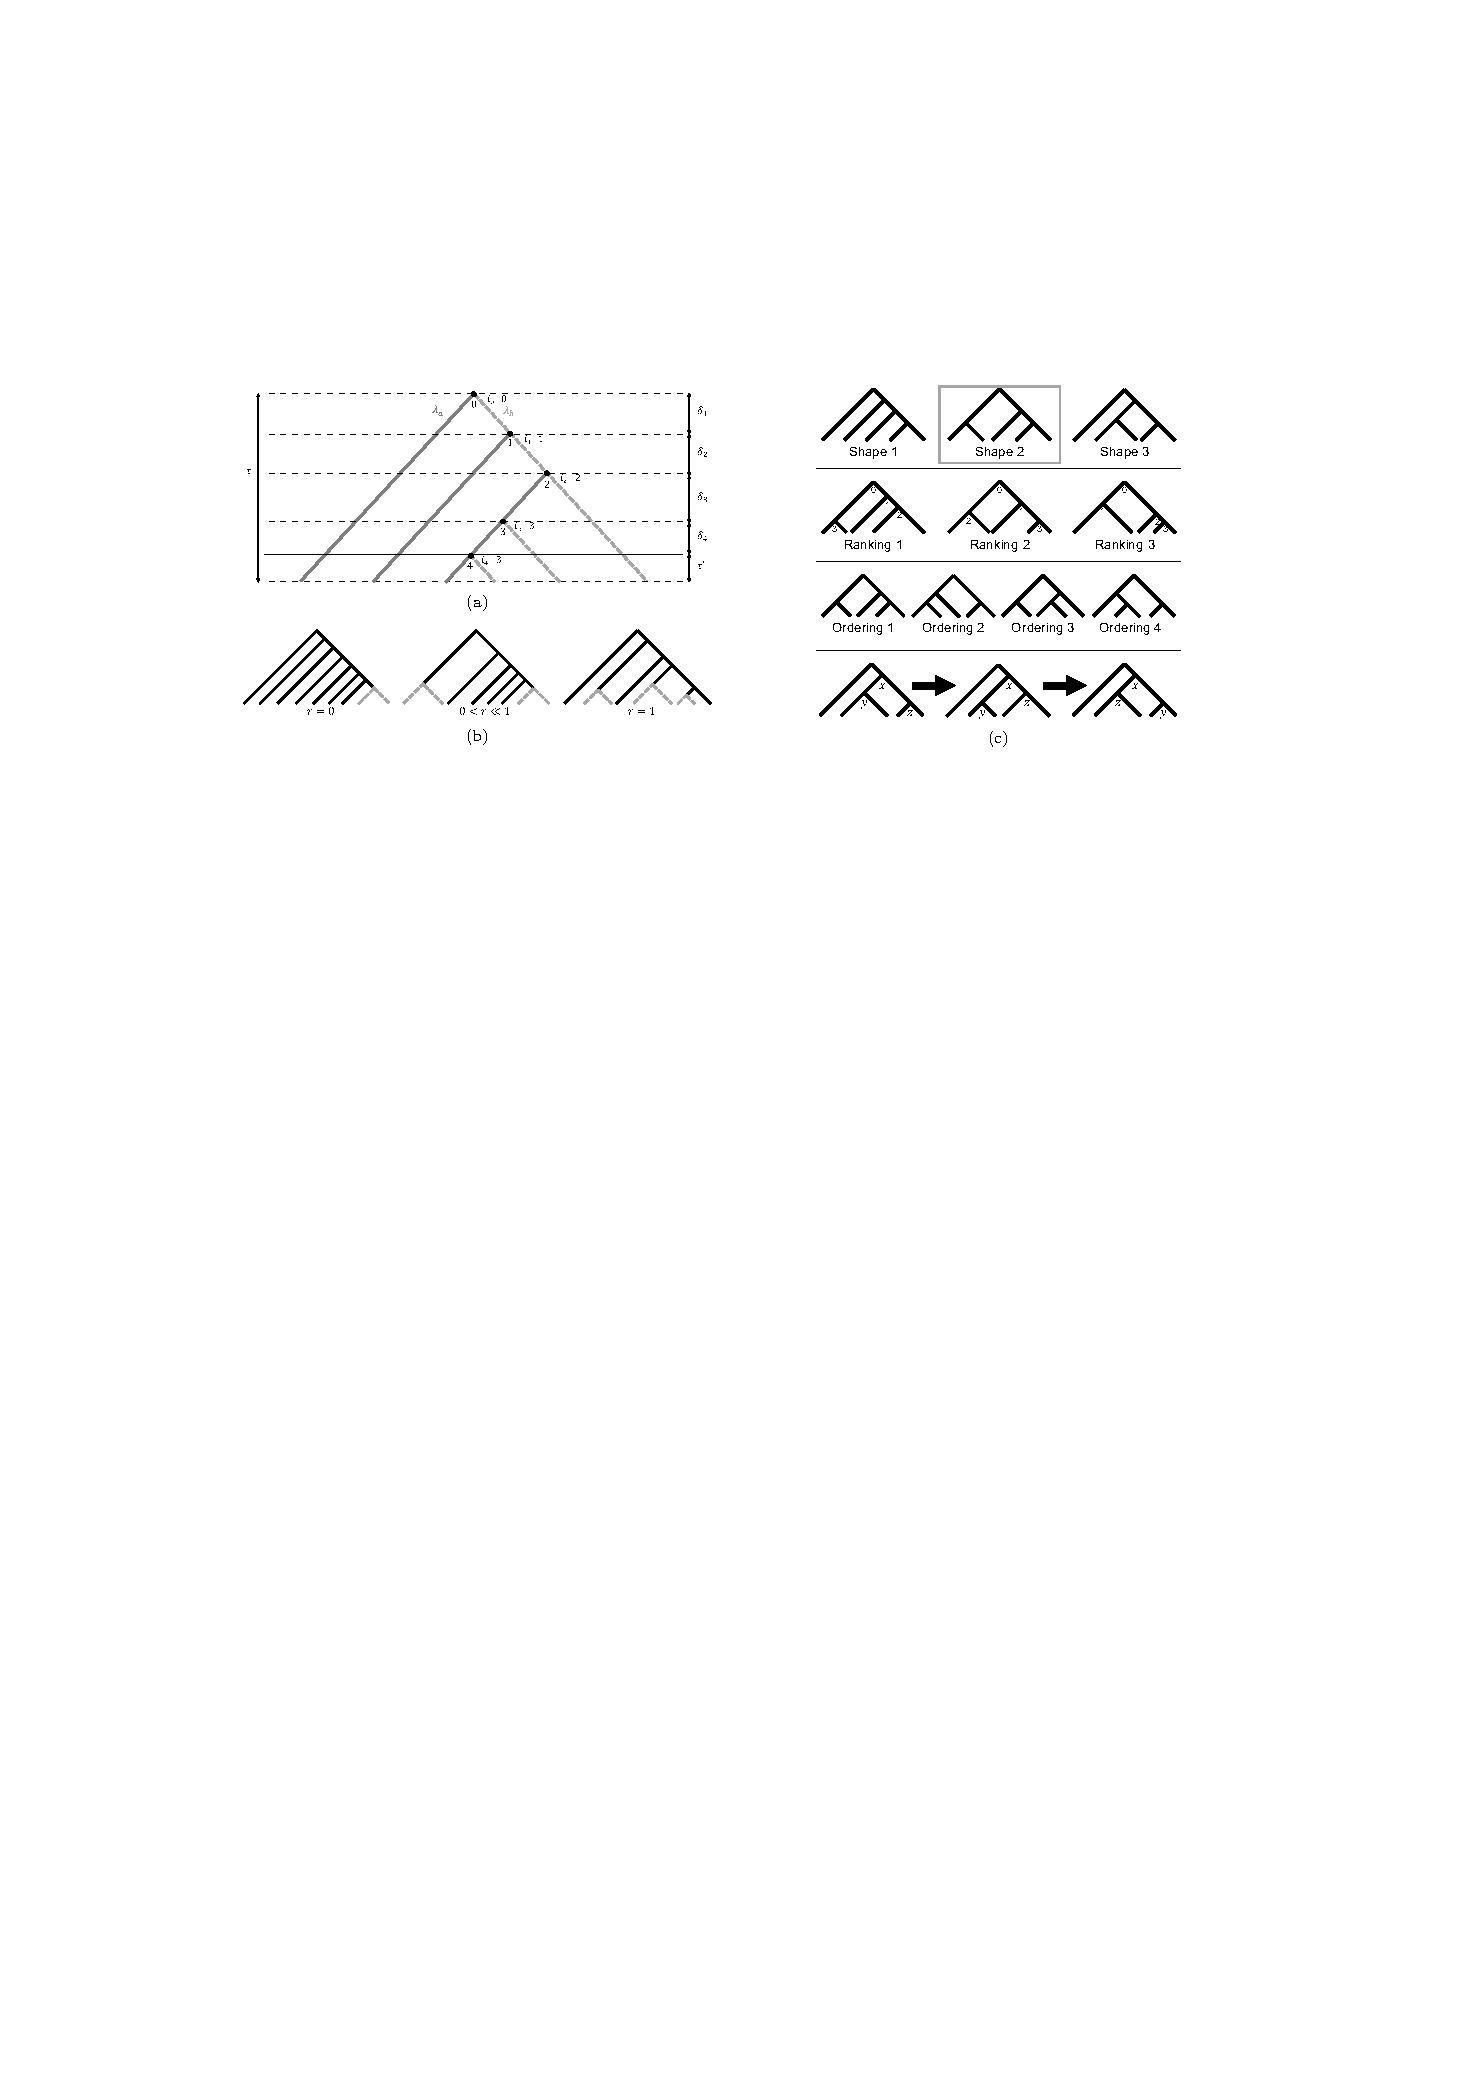
\includegraphics[width=\textwidth]{figs/dualbirth-model}
\caption[Dual-birth model]
{Dual-birth model. (a) A caterpillar tree with one cherry (node 4). The tree is generated by the dual-birth model; right branches (dashed light gray) are sampled from the Poisson process with rate $\lb$, and left branches (solid dark gray) are sampled with rate $\la$. Internal nodes are ranked by distance to the root (ranks shown below nodes), and the tree is divided into time intervals between consecutive nodes. (b) With $r=\la/\lb=0$, only caterpillar trees can be generated; as r increases toward $1$, the tree becomes more balanced and thus has more cherries (dashed light gray). (c) All three possible tree shapes with five leaves are shown on top; the second row shows $\RNALL$, all possible rankings of tree shape 2; the third row shows $\SDALL$, all orderings of tree shape 2. The last row demonstrates that, starting from a ranked ordered tree, one change of ranking followed by a change of ordering results in a tree identical to the original tree.}
\label{fig:dualbirth-model}
\end{figure}

\subsection{Theoretical Properties of the Dual-Birth Model}\label{sec:dualbirth-meth}
\subsubsection*{Notations and definitions}
A connected \gls{DAG} with no undirected cycles defines a tree. We only consider binary trees in which all nodes either have outdegree zero (leaves) or two (internal nodes). Two trees are considered to have the same \textit{shape} if there exists a one-to-one mapping between their nodes such that the head and tail of every edge in one tree map to the head and tail of exactly one edge in the other tree. In this paper, we care about the space of distinct tree shapes. In the tree-shape space, leaves are not distinguished (i.e., a tree shape is unlabeled). For simplicity of presentation, we represent a tree shape on $n$ leaves using $T=(V,E)$, where $V$ is the set of $n-1$ \textit{internal} nodes and $E$ is the set of internal edges $(u,v)$ from parent node $u$ to child node $v$. Note that terminal edges (connecting internal nodes to leaves) and leaves are not part of $E$ and $V$, and as such, are implicit in the $T$ formulation (each internal node has to have outdegree two). We use $\child{u}{1}$ and $\child{u}{2}$ to denote the children of $u$, and we use $\leaf$ to denote a generic unlabeled leaf. Note that $T$  defines a \gls{POSET} on $V$.

Recall a node $v\in V$ is called a cherry if both of its children are leaves. A tree shape is called \textit{caterpillar} if it has only one cherry (Fig.~\ref{fig:dualbirth-model}a); in contrast, a fully-balanced tree has exactly $n/2$ cherries. The number of cherries of a tree is denoted as $\CH{T}$.

Let $\NV\defeq\{0,1,\ldots, n-2\}$. A bijective function $\RN:V\mapsto\NV$ is a ranking of a tree $T=(E,V)$  if for each edge $(u,v)\in E$, we have $\RN(u)<\RN(v)$. A \textit{ranked tree shape} is defined as $\TR\defeq (T,\RN)$. Each ranking is a topological sorting of the tree (i.e., is a linear extension of the \gls{POSET} defined by the tree shape). We use $\RNALL(T)$ to denote the set of all possible rankings of the tree shape $T$ (Fig.~\ref{fig:dualbirth-model}c).

An \textit{ordered tree shape} is a tree shape in which left and right child nodes are distinguished (i.e., the tree is oriented). More precisely, $\SD:V\mapsto\{0,1\}$  is a valid order for a tree shape $T$ iff $\SD(\child{u}{1})+\SD(\child{u}{2})=1$ for every $(u,\child{u}{1}),(u,\child{u}{2})\in E$ and $\SD(r)=1$ for the root node $r$. We call $v$ a left child/node when $\SD(v)=0$ and otherwise call it a right child/node. A branch leading to a left (right) child is called a left (right) branch. An ordered tree shape is denoted by $\TO\defeq(T,\SD)$. Note that, in this definition, leaves are not directly assigned a left/right side. Leaves below a cherry are indistinguishable; leaves that are sister to internal nodes are considered to have the opposite side of their sibling. For example, in Figure~\ref{fig:dualbirth-model}a, the leaf directly below the root is considered a left node because its sister, the node ranked 1, is a right node. Also, $\SDALL(\TR)$ denotes the set of all possible orderings that are valid for $\TR$ (Fig.~\ref{fig:dualbirth-model}c).

A ranked ordered tree shape is defined by $\TRO\defeq(T,\RN,\SD)$. For ease of notation, we define $\SD_i\defeq\SD\left(\RN^{-1}(i)\right)$ (the order of the node ranked $i$). For $0<i<n$ and the ranked ordered tree $\TRO$, we define $\LB{i}(\TRO)\defeq1+\sum_{k=1}^{i-1}\SD_k$ and it is easy to show that $\LB{i}(\TRO)$ gives the number of left branches $(u,v)$ with $\SD(u) < i$ and $\SD(v) \geq i$. In other words, $\LB{i}(\TRO)$ gives the number of left terminal branches if the tree $\TRO$ is terminated at the time when node $i$ is created. Where clear by the context, we simply write $\LB{i}$ (Fig.~\ref{fig:dualbirth-model}a). We define $\LBh\defeq\LB{n-1}$ and $\RBh\defeq n-\LBh$; these definitions can be intuitively considered to show the number of left and right terminal branches, respectively, if we assign an order to all terminal branches (e.g. $\RBh=\LBh=3$ in Fig.~\ref{fig:dualbirth-model}a).

We refer to a tree shape with ultrametric branch lengths as a weighted shape. A weighted shape is defined by $t\defeq(T,\bl,\tau)$, where $\bl:E\mapsto\mathbb{R}$ gives the length of internal branches and $\tau$ gives the distance from the root to all leaves; note that $\tau$ has to be larger than the largest distance to the root from any internal node. Node ages define a unique ranking on any weighted shape. A weighted shape $t$ can also be assigned an order, $\SD$, and will be denoted by $\tO$. For $e=(u,v)\in E$, we refer to  $\bl(e)$ by $\bl_i$ where $i={\RN(v)}$ (e.g. $\bl_1\ldots\bl_4$ in Fig.~\ref{fig:dualbirth-model}a).

\subsubsection{Probability Distributions}
We now derive probability distributions on tree shapes conditioning on fixed $n$. Here we give the main results and provide the proofs in Section~\ref{sec:dualbirth-proofs}.

\begin{theorem}\label{thm:TRO}
Let $X$ be a random variable (r.v.) over ordered ranked tree shapes and distributed according to the dual-birth model with parameter $r=\la/\lb$. Then, 
\begin{equation}\label{eq:orts}
\Pr(X=\TRO;n) = \frac{r^{\RBh-1}}{\prod_{i=1}^{n-2} \big((r-1)\LB{i}+i+1\big)}
\end{equation}
\end{theorem}

Computing Equation~\ref{eq:orts} simply requires knowing the number of right leaves ($\RBh$) and the number of its left branches if the tree is terminated at each node $i$ ($\LB{i}$); all of these can be computed in time $O(n)$ for an ordered tree. Figure~\ref{fig:dualbirth-tree-prob-dists} shows the perfect match between Equation~\ref{eq:orts} and observed frequencies in simulations for all ranked ordered tree shapes with $n=6$ and shows that, with $r\ll1$, the caterpillar tree shape has a high probability.

The left/right order of nodes cannot be estimated from sequence data, and thus, it would be more useful to compute the probability distribution over unordered ranked tree shapes. Since all orderings of a \textit{ranked} tree are distinct, the probability of a ranked tree simply needs to marginalize over all possible orderings. Thus,
\begin{corollary}
For $Y$, an r.v.\ over ranked tree shapes with $n$ leaves and distributed according to the dual-birth model,
\begin{equation}\label{eq:rts}
\Pr(Y=\TR;n) = \sum_{\SD\in\SDALL(\TR)} \Pr(\TRO)
\end{equation}
where $\SDALL$ gives the set of all orderings of $\TR$.
\end{corollary}

This computing requires an exponential number of computations to iterate all orderings (the recursive formula for that iteration is given in Equation~\ref{sup:eq:sdall}. Whether efficient algorithms for computing this probability exist is unclear to us. See Figure~\ref{fig:dualbirth-tree-prob-dists} for an example distribution and matching simulations.

Next, we turn to computing the probability distribution over unranked shapes. This can be done by enumerating all possible rankings of the unranked tree and summing up their probabilities. The set of all rankings, $\RNALL(T)$, is simply the set of all the linear extensions of the \gls{POSET} defined by the tree shape. However, a final complication needs to be addressed. Recall that leaves are unlabeled. For a non-cherry symmetric node $u$ (i.e., sub-tree shapes below $\child{u}{1}$ and $\child{u}{2}$ are identical), take any ordering of any ranking of nodes below $u$. Now swap $\SD(\child{u}{1})$ and  $\SD(\child{u}{2})$ and also swap the rankings of nodes below $\SD(\child{u}{1})$ with the rankings of the identical nodes under $\SD(\child{u}{2})$ (Fig.~\ref{fig:dualbirth-model}c); this would produce an identical tree shape. However, our process will count this identical tree shape twice. To account for this, we need to divide the total probability by two for every non-cherry symmetric node. Thus,
\begin{corollary}
For $Z$, an r.v.\ over tree shapes with $n$ leaves and distributed according to the dual-birth model,
\begin{equation}\label{eq:rt}
\Pr(Z=T;n) = \frac{1}{2^{\sigma(T)}}\sum_{\RN\in\RNALL(T)} \Pr(\TR)
\end{equation}
where $\RNALL$ gives all rankings of $T$ and $\sigma(T)$ is the number of non-cherry symmetric nodes in $T$.
\end{corollary}

\subsubsection{Weighted Trees}
Given an ordered weighted tree shape $\TRO$, we can easily compute the probability density function (p.d.f) for the length of each of its internal branches. Recall $\bl_i$ is the time between internal nodes ranked $i-1$ and $i$ (i.e., an interval), which is simply the length of a specific branch. Given the tree shape, $\bl_i$  follows an exponential distribution with rate $\li=\la\LB{i}+\lb(i+1-\LB{i})$. This is because the branch length is simply the  minimum of all exponential r.v.s active in the corresponding interval, which itself, is an exponential r.v. with the total rate. Furthermore, since each interval is independent of the other intervals given $\TRO$, the joint probability density of $\TRO$ and a set of internal branch lengths can be computed by multiplying the probability of $\TRO$ (Eq.~\ref{eq:orts}) by the probability density of every branch length given $\TRO$. Finally, to compute the joint probability density of a given tree and all its branch lengths, we need to also multiple the probability of no births in the final interval of length $\bl_{n-1}=\tau-\sum_1^{n-2}\bl_{i}$; this is the probability of no events for an exponential with rate $\LB{n-1}$ in time $\bl_{n-1}$; i.e., $e^{-\LB{n-1}\bl_{n-1}}$.

\subsubsection{Expected Number of Cherries and Active Leaves}\label{sec:cherries}
We now ask the following question: how many cherries and how many active nodes are expected in a dual-birth tree generated with rate ratio $r$?

A parsimony analysis is constructive here. Activation events can be considered evolutionary changes. Given an unordered tree, the most parsimonious ordering is one that implies the minimum number of activation events. The number of activations is simply the number of left branches that have children. By making every internal node that is sister to a leaf a right node and arbitrarily ordering the rest, one can show that the most parsimonious ordering has exactly one activation for each cherry in the tree, counting the root as an activation (Lemma~\ref{lem:cherryparsimony}). The parsimony analysis would only be relevant for $r\ll1$, when one would expect very few activations. As $r$ increases, the tree becomes more balanced, and we would expect more cherries. We now formalize this intuition.

\begin{theorem}\label{thm:cherr}
For a tree shape $Z$ generated by the dual-birth model with $r=\la/\lb$, let $C=\CH{Z}/n$ be an r.v. capturing the fraction of cherries; then, 
\begin{align}\label{eq:cherries}
\lim_{n\to\infty}\mathbb{E}(C) = \frac{\sqrt{r}}{1+r+\sqrt{r}}
\end{align}
\end{theorem}

\begin{corollary}\label{cor:rbh}
For an r.v.\ $N_r$ capturing the fraction of right (i.e., active) leaves in tree shape $T$,
\begin{align}\label{eq:nr}
\lim_{n\to\infty}\mathbb{E}(N_r) = \frac{\sqrt{r}}{1+\sqrt{r}}
\end{align}
\end{corollary}

\begin{figure} % FIGURE 2 IN ORIGINAL PAPER
\centering
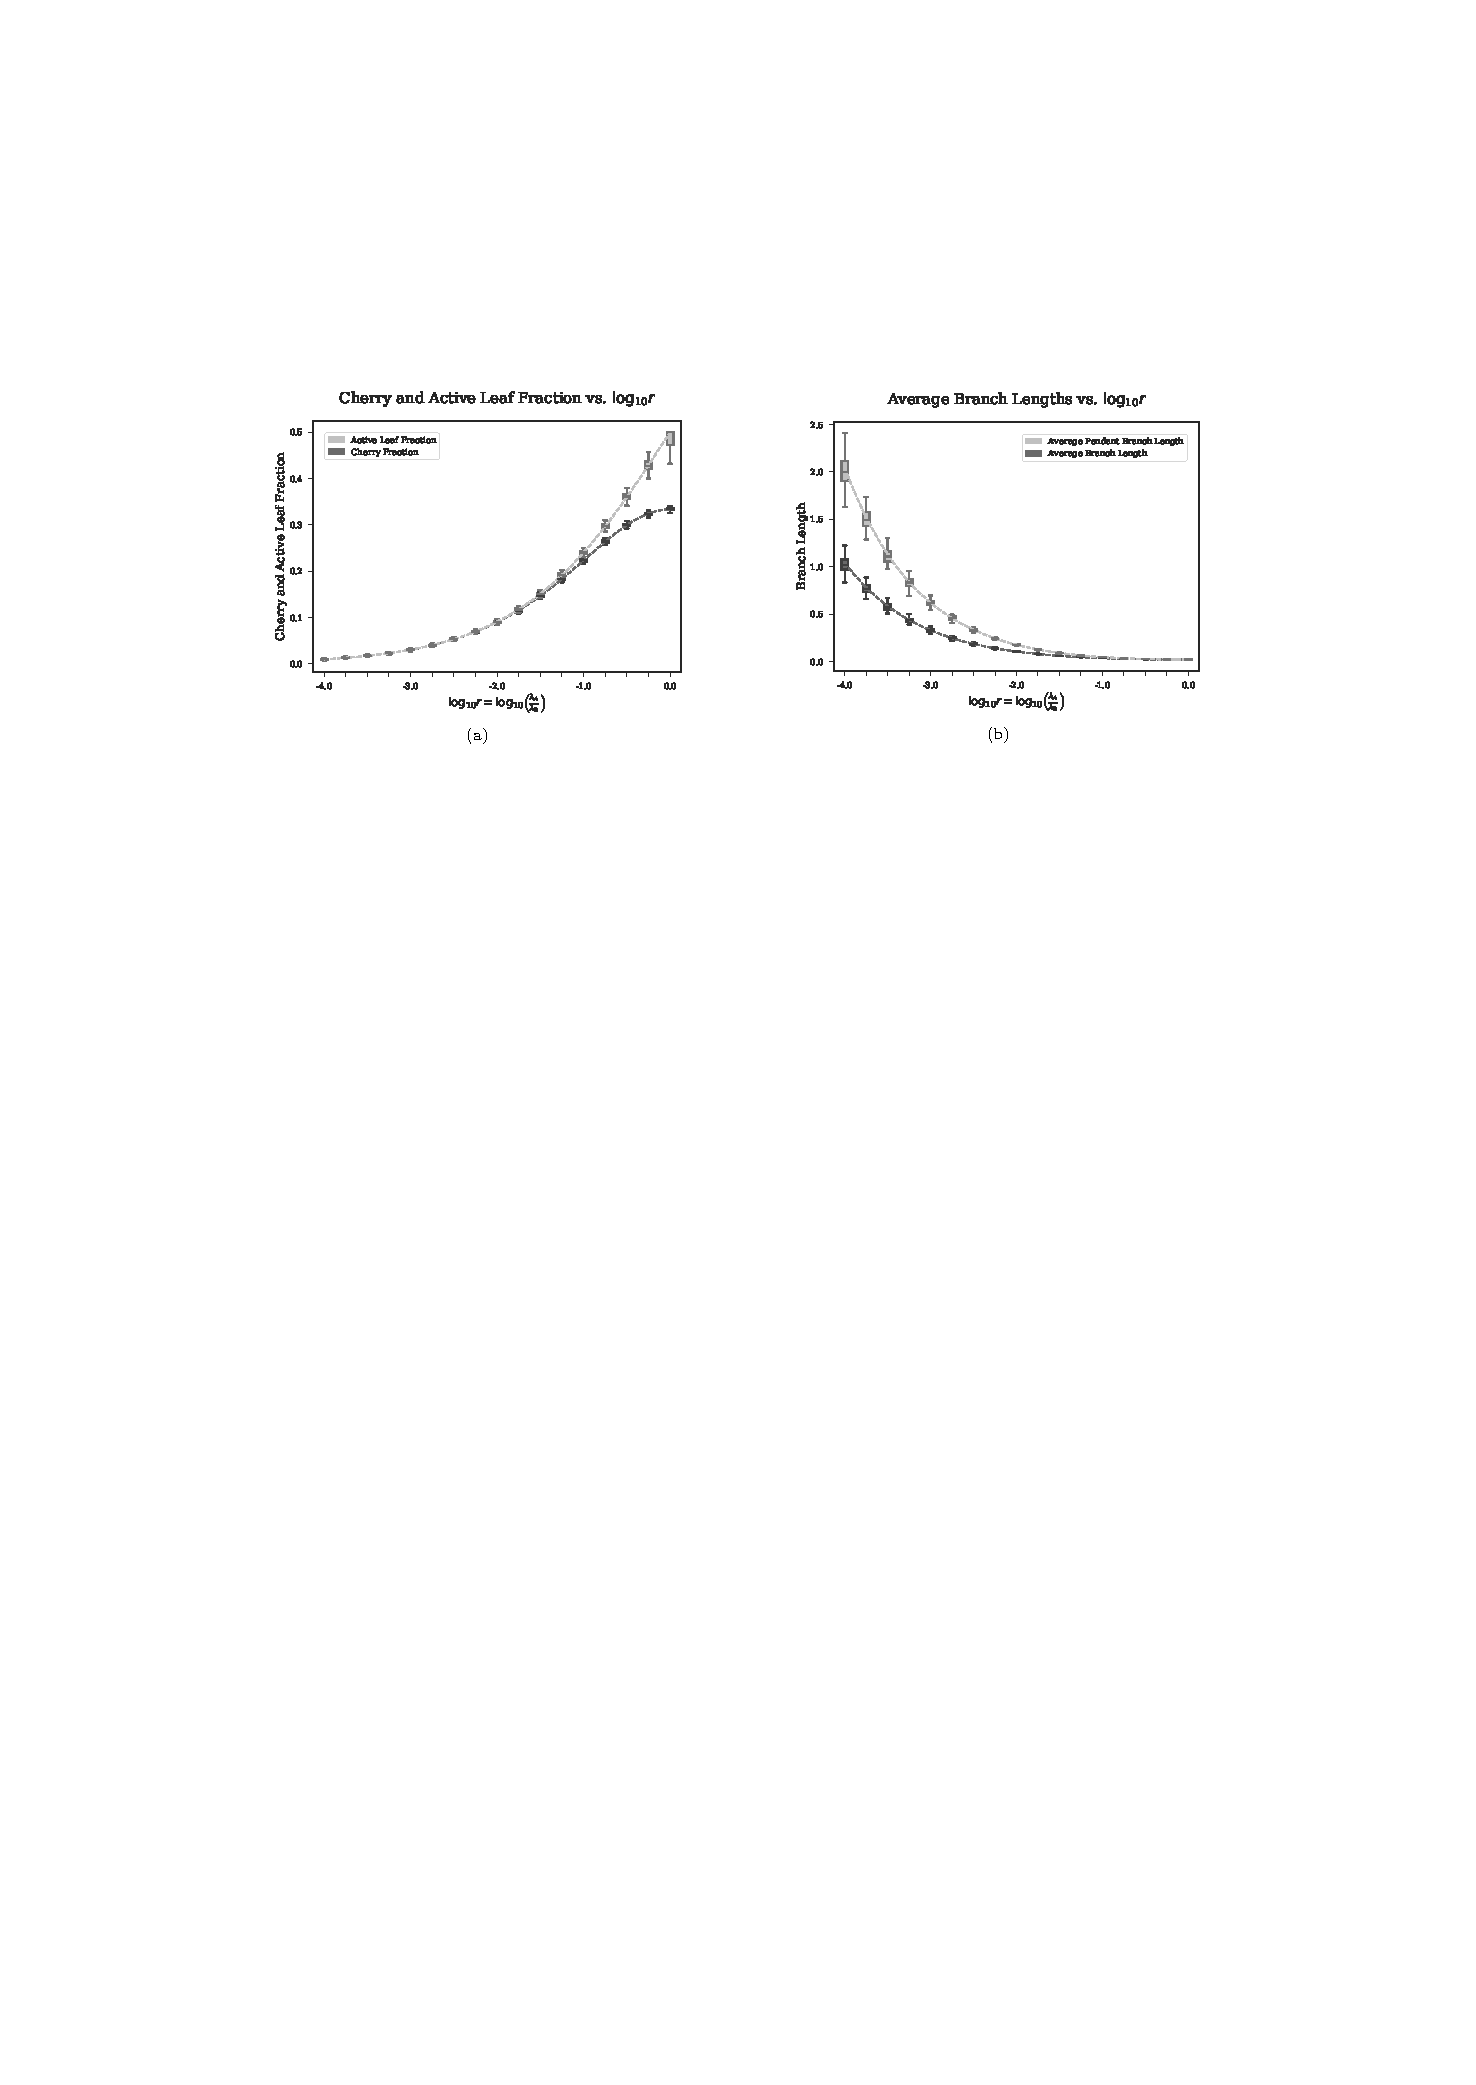
\includegraphics[width=\textwidth]{figs/dualbirth-c-vs-r}
\caption[Theoretical Expectations]
{Theoretical expectations of (a) cherry fraction (dashed dark gray line) and active leaf fraction (dashed light gray line), and (b) branch length (dashed dark gray line) and pendant branch length (dashed light gray line) versus simulated distributions (in box plots) using 100 replicates with $n=4096$, $\lambda=48$, and varying values of $r$ ($x$-axis) from $1/1024$ to $1$. Note that the number of cherries is the maximum parsimony estimate of the number of active elements, and the most parsimonious estimate works well for low values of $r$.}
\label{fig:dualbirth-c-vs-r}
\end{figure}

The proofs can be found in Section~\ref{sec:dualbirth-proofs}.
As Figure~\ref{fig:dualbirth-c-vs-r}a shows, these expectations closely match simulations results. As $r$ increases, the expected frequency of cherries increases until it reaches its peak at \sfrac{1}{3} for $r=1$. The number of active elements follows a similar pattern and reaches its peak at \sfrac{1}{2}  for $r=1$. Thus, under the Yule model, only half the nodes will be expected to be active (recall that an active element is defined as one that has already propagated). Also note $r=x$ and $r=\frac{1}{x}$ differ only in what elements are labeled left or right, and thus, they are indistinguishable for unordered trees. As noted before, $r>1$ does not have a meaningful interpretation in biological processes that we consider; thus, we focus on $0\leq r\leq1$.

\subsubsection{Expected Branch Length}
A natural quantity of interest under any model of tree evolution is the expected length of a random branch. For example, under the Yule model, branches are exponentially distributed with rate $1/2\lambda$~\cite{Mooers2012}. In our model, the expected branch length depends on both $\lambda$ and $r$. In all the results given below, we assume all the leaves are sampled. 
\begin{theorem}\label{thm:bl}
For a weighted tree shape $t$ generated by the dual-birth model with parameters $r$ and $\lambda$ conditioned on having $n$ leaves, let $\BL$ be an r.v.\ giving the length of a random branch in $t$; i.e., $\BL=\bl_I$ for $I\sim\mathcal{U}(1,n-2$). Then, 
\begin{align}\label{eq:bl}
\lim_{n\to\infty}\mathbb{E}(\BL) \to \frac{1}{2\lambda}\left(\frac{r+1}{\sqrt{r}}\right) = \frac{1}{\la}\frac{\sqrt{r}}{2}
\end{align}
\end{theorem}

The proof can be found in Section~\ref{sec:dualbirth-proofs}. For a fixed $\lambda$, increasing $r$ in $(0,1]$ reduces the expected branch lengths, resulting in the minimum value under the Yule model (Fig.~\ref{fig:dualbirth-c-vs-r}b).

\subsubsection{Expected Terminal Branch Length}
Under the Yule model, terminal and internal branch lengths have the same expected length~\cite{Mooers2012}. For $r\ll1$, we expect that inactive entities result in long terminal branches and relatively short internal branches. These expectations can be confirmed in simulations. As expected, close to $r=1$, the mean terminal branch length is close to the mean branch length but the two values gradually diverge as $r$ decreases (Fig.~\ref{fig:dualbirth-c-vs-r}b). Therefore, the difference between average terminal and internal branch lengths is a function of $r$, and therefore, a closed-form formula for the expected terminal branch length would be useful in building an estimator of $r$. While we don't have a proven result for the terminal branch length, based on simulations, we present a conjecture. Note that this conjecture was purely reached based on our intuition and trial-and-error, starting from Equation~\ref{eq:bl} and modifying the denominator until a close match to the empirical values was obtained.

\begin{conjecture}\label{thm:tbl}
For a weighted tree shape $t$ generated by the dual-birth model with parameters $r$ and $\lambda$ conditioned on having $n$ leaves, let $\TBL$ be an r.v.\ giving the length of a random terminal branch in $t$. Then, 
\begin{align}\label{eq:tbl}
\lim_{n\to\infty}\mathbb{E}(\TBL)\to\frac{1}{\la}\left(\frac{\sqrt{r}}{1+2\sqrt{r}-r}\right)
\end{align}
\end{conjecture}

Figure~\ref{fig:dualbirth-c-vs-r}b shows that the conjectured results closely match the observed mean terminal branches for a wide range of $r$ values. Note that changing $\la$ simply scales all lengths, so our simple simulations have explored \textit{all} free parameters of the dual-birth model (albeit, only for $r\in[10^{-4},1]$ range). Regardless of whether our conjecture is true (which cannot be proven by simulations), the close match of Equation~\ref{eq:tbl} and simulated results means that we can use it to provide an approximate estimator of $r$.

\subsubsection{Parameter Estimation}\label{sec:paramest}
Theorem~\ref{thm:cherr} enables us to estimate the $r$ parameter for a given tree. Given a tree with $c$ cherries, and for $x=c/n$, solving for $r$ in Equation~\ref{eq:cherries} results in the following relationship (Fig.~\ref{fig:dualbirth-sup-cvsr}):
\begin{equation}\label{eq:rforc}
\hat{r}(x)=\bigg(\frac{1-x-\sqrt{(x+1)(1-3x)}}{2x}\bigg)^2
\end{equation}
for $x\leq \frac{1}{3}$ and else $\hat{r}(x)=1$.

An alternative estimator can be designed by combining Theorem~\ref{thm:bl} and Conjecture~\ref{thm:tbl} for expected total and terminal branch length. Given a tree with an average branch length of $d$ and an average terminal branch length of $l$, solving Equations~\ref{eq:bl}~and~\ref{eq:tbl} for $r$ and $\lambda_a$, we can design the following estimator for large $n$:
\begin{equation}\label{eq:rforbl}
\hat{r}(b,l) = \left(1-\sqrt{2\left(1-\frac{d}{l}\right)}\right)^2
\end{equation}

Further approximating the total average branch length to be the mean of internal branch lengths ($i$) and terminal branch lengths (a good approximation for large $n$), we can further simplify Equation~\ref{eq:rforbl} to:
\begin{equation}\label{eq:rforbl-approx}
\hat{r}(i,l) = \left(1-\sqrt{1-\frac{i}{l}}\right)^2
\end{equation}

Having estimated $r$, we can easily use Equation~\ref{eq:bl} to get an estimate of $\lambda$ from the observed mean branch length for large $n$. Note that, absent a proof for Conjecture~\ref{thm:tbl}, Equation~\ref{eq:rforbl} should be treated as an approximate estimator. Also note that this approximate estimator assumes the given tree itself was generated by the dual-birth model (e.g. it is not the result of subsampling the tips of a tree generated by the dual-birth model). We discuss statistical properties of both estimators in Section~\ref{sec:dualbirth-discussion}. 

\subsubsection{Sampling the Dual-Birth Model}\label{sec:samplingalgo}\label{sec:db-algo}
When conditioning on $n$, the number of tips, a simple algorithm can be used to sample the space of ordered weighted tree shapes defined by the dual-birth model.

We start with a single-node tree and iteratively add new nodes until the tree has $n$ leaves. We use a heap to keep a list of current leaves sorted by their distance to the root. In each iteration, we add two child nodes to the highest leaf in the tree (i.e., the leaf closest to the root); we sample from two exponential distributions with rates $\la$ and $\lb$ for the left and right child's branch lengths, respectively. The two new nodes are added to the heap of leaves, and the parent is removed from the heap. Once the loop has terminated, we truncate the tree by shrinking all terminal edges except the one attached to the leaf that is closest to the root such that all leaves are equidistant to the root.

%\paragraph{Correctness:}
Hartmann \textit{et al}. have described various strategies for sampling trees with $n$ leaves~\cite{Hartmann2010}. Our sampling procedure falls under what they have termed \gls{SSA}. As they point out, the \gls{SSA} procedure produces the right distribution on tree topologies for pure birth models, like ours, because, once the process reaches $n$ tips for the first time, it never goes back to having fewer tips. A remaining question is what distribution should be used to decide the time between when $n$ leaves first become present until we stop the simulation (call it $\tav$). Let $h(\tav)$ be the p.d.f of that waiting time. If the time between when we have $n$ leaves and the the birth of leaf $n+1$ is given by $x>\tav$, then $\tav$ should be uniformly sampled between zero and $x$. Moreover, the probability of sampling each tree with $n$ leaves should be proportional to $x$, the time it remains an $n$-leaf tree. Thus, as Hartmann \textit{et al}.show, by summing over all possible values of $x$, we get:
\begin{small}
\begin{eqnarray}\label{eq:h}
h(\tav) \propto \int_{x=\tav}^{\infty} x.h(\tav|x).g_{n-1}(x) \ \mathrm{d}x &=& \int_{x=\tav}^{\infty} x.\frac{1}{x}.g_{n-1}(x) \ \mathrm{d}x  \nonumber \\ 
&=& \int_{x=\tav}^{\infty} g_{n-1}(x) \ \mathrm{d}x
\end{eqnarray}
\end{small}
where $g_{n-1}$ is the p.d.f of a random variable (r.v.) for $x$. In our model, this r.v.\ is equivalent to the minimum of $n$ exponential r.v.s, $\LB{n-1}$ of which have rate $\la$ and the rest have rate $\lb$; thus, $g(x)$ is the p.d.f of an exponential with rate $\lambda_{n-1}=\lambda_a \LB{n-1}+\lambda_b(n-\LB{n-1})$. It is easy to see that Equation~\ref{eq:h} simplifies to $h(\tav)\propto g_{n-1}(\tav)$. Thus, the correct waiting time between the last birth event and the end of the simulation is identical to the waiting time for the birth event that would create $n+1$ leaves.

Note that, if we were conditioning on $\tau$ (the tree height) instead of $n$, the same procedure would remain correct, except we would continue until all leaves have at least the required height and would then cut branches that are longer than $\tau$.

\subsection{Simulation Setup}
\subsubsection{Datasets}
Given a set of parameters, we use our implementation of the fixed-$n$ sampling procedure  to generate 20 replicate ``true'' trees. We then deviate each tree from ultrametricity by multiplying each branch of the tree by a multiplier sampled from a gamma distribution with shape and rate both set to $\alpha$ (with an expected value of 1). For each true tree, we then use INDELible~\cite{Fletcher2009} and the \gls{GTR}+$\Gamma$ model~\cite{Tavare1986} to simulate a multiple sequence alignment with no indels, which is later used to infer the tree. The simulation parameters are \textit{n}, $r$, $\lambda$, and deviation from ultrametricity (i.e., the shape of the Gamma distribution, $\alpha$). For sequence evolution, the parameters to select are $k$ (the sequence length), the \gls{GTR} parameters, and the Gamma rate across sites. We also vary model of sequence evolution used for inference.

\begin{table}[!ht] % TABLE 1 IN ORIGINAL PAPER
\caption[Experiments]{Experiments (default parameters in bold)}
\vspace{-0.25in}
\begin{center}
\begin{tabular}{|l|l|l|}
\hline
{\bf\#}&{\bf Parameter} & {\bf Parameter Values}\\
\hline
1&$r$ (const. bl) & $10^{-4}, 10^{-3}, {\bf 10^{-2}}, 10^{-1}, 10^{0}$\\
2& Model & JC69, K80, HKY85, GTRCAT, \textbf{GTR+$\Gamma$}\\
3&$\lambda$ & $33.866, 84.664, {\bf 169.328}, 338.655, 846.64$\\
4&$k$ & $50, 100, 200, {\bf 300}, 600, 1200, 2400, 4800$\\
5&$n$ & $25, 50, 250, 500, {\bf 1000}, 2000, 4000$\\
6& $\alpha$ (clock) & $2.952, 5.904, {\bf 29.518}, 147.591, 295.182, \infty$\\
\hline
\end{tabular}
\end{center}
\label{tab:dualbirth-experiments}
\end{table}

%% END DUAL-BIRTH CHAPTER
\newcommand{\PLH}{H$^+$I\xspace}
\newcommand{\PLWH}{SH$^+$I\xspace}

%% START PROACT CHAPTER
\chapter{\proacttitle}
\label{chap:proact}
\clearpage

In \gls{HIV} epidemics, the majority of the structure of the transmission network is dictated by just a few individuals. Public health intervention, such as ensuring people living with \gls{HIV} adhere to \gls{ART} and are continually virally-suppressed, can help control the spread of the virus. However, such intervention requires utilizing the limited public health resource allocations. As a result, the ability to determine which individuals are most at-risk of transmitting \gls{HIV} could allow public health officials to focus their limited resources on these individuals. Molecular epidemiology suggests an approach: prioritizing people living with HIV based on patterns of transmission inferred from their sampled viral sequences. In this paper, we introduce ProACT (\textbf{Pr}i\textbf{o}ritization using \textbf{A}n\textbf{C}es\textbf{T}ral edge lengths), a novel phylogenetic approach for prioritizing individuals living with \gls{HIV}. ProACT uses a simple idea: ordering individuals by their terminal branch length in the phylogeny of their virus. In simulations and also on a dataset of \gls{HIV}-1 subtype B \textit{pol} sequences obtained in San Diego, we show that this simple strategy improves the effectiveness of prioritization compared to state-of-the-art methods that rely on monitoring the growth of transmission clusters defined based on genetic distance.

\section{Introduction}
The transmission of \gls{HIV} resembles scale-free networks~\cite{Wertheim2014}, in which the majority of the structure of the network is dictated by just a few individuals, a phenomenon likely resulting from the scale-free properties of sexual contacts and injection drug use along which \gls{HIV} is transmitted~\cite{Little2014,Schneeberger2004}. As a result, public health intervention may be more effective when targeted at people living with \gls{HIV} who are more likely to grow the transmission network. However, the best method to target individuals for specific interventions remains an open question, and the best strategy will likely depend on the specific intervention planned.

A potential form of intervention aiming to reduce future transmissions is to target \glspl{PLH}. For example, \gls{ART} suppresses the \gls{HIV} virus in the majority of cases, stops the progression of the disease, and prevents onward transmission to an uninfected sexual partner, provided the \gls{PLH} continuously adheres to the treatment~\cite{Cohen2011}. In addition to reducing risk of transmission at the molecular level, adherence to \gls{ART} is associated with a reduction of risky behavior as well~\cite{Bunnell2006}. While the initiation of \gls{ART} is routine (or even universal) in most advanced health care systems, not every case of \gls{ART} initiation leads to a sustained suppression of the virus through time. \glspl{PLH} who start \gls{ART} but fail to sustain it or who are otherwise unsuppressed can still infect others. Thus, a possible intervention is to ensure known \glspl{PLH} are kept on \gls{ART} and are continually suppressed, a task that requires allocation of public health resources. If people at risk of losing their suppression could be predicted accurately, the public health system could focus their limited resources on these individuals, administrating several types of interventions: followups to ensure sustenance of \gls{ART}, increased testing to ensure suppression, and, if all else fails, offering \gls{PrEP} to their sexual partners. However, these are all costly interventions and cannot be undertaken for every known \gls{PLH}. Thus, a natural question surfaces: which individuals are most at-risk of transmitting \gls{HIV}?

Predicting tendency for future transmissions is difficult and is fraught with danger if undertaken primarily based on demographic or behavioral traits. Molecular epidemics suggest an alternative method: prioritizing \glspl{PLH} for intervention solely based on patterns of transmission inferred from \gls{HIV} sequence data~\cite{Bbosa2019,Villandre2019,Oster2018,Ragonnet-Cronin2019,Wertheim2018,Wertheim2011,Wertheim2014,Smith2009}. The inference of transmission networks using phylogenetic or distance-based methods has been the subject of much research~\cite{Leitner2018,Pond2018,Ragonnet-Cronin2013,Prosperi2011}. However, in this work, instead of being concerned with inferring exact patterns of transmissions, we ask the following question: given molecular data from each \gls{PLWH}, presumably all with access to \gls{ART}, which individuals are most at-risk of transmitting the virus?

Prioritizing care based on molecular epidemics has been studied recently. Wertheim \textit{et al}. (2018) present a method for prioritizing \glspl{PLWH} based on performing transmission clustering (i.e., grouping individuals with low viral genetic distance into ``transmission clusters'') and ordering clusters  by growth rate~\cite{Wertheim2018}. On a large dataset from New York, they show that the approach is able to predict individuals who will have relatively larger numbers of transmission links in the near future. Moshiri \textit{et al}. (2018) have studied the same question in simulations and have shown that monitoring cluster growth can be used for predicting future transmissions substantially better than a random guess, whether clusters are defined using genetic distances or using phylogenetic methods~\cite{Moshiri2018}. Most recently, Balaban \textit{et al}. (2019) showed in simulations that using a cluster-monitoring approach similar to that of Wertheim \textit{et al}. (2018) but defining clusters  using a min-cut optimization problem gives a small but consistent improvement over defining clusters using genetic distances~\cite{Balaban2019}.

In this paper, we introduce a new method for ordering \glspl{PLWH} based  on their phylogenetic relationships. Instead of relying on clustering individuals and then ordering clusters based on their growth, we seek to order individuals without clustering and without reliance on parametric models. Instead, we seek to simply exploits patterns in the phylogeny, and in particular, in branch lengths.

\section{New Approaches}
ProACT (\textbf{Pr}i\textbf{o}ritization using \textbf{A}n\textbf{C}es\textbf{T}ral edge lengths) takes as input the inferred phylogenetic relationships between sampled \gls{HIV} viruses (e.g. from the \gls{pol} region), rooted using an outgroup or clock-based methods (e.g. midpoint or MinVar-root~\cite{Mai2017}). ProACT simply orders \glspl{PLWH} in order of incident branch length of their associated virus, and it breaks ties based on incident branch lengths of parent nodes, then those of grandparent nodes, etc. We first motivate the approach and then present a formal definition of the method.

We note that ProACT is motivated and tested in a context similar to the present day health care systems that enjoy enough resources to provide \gls{ART} to all \glspl{PLWH} (recall that we call a \gls{PLH} a \gls{PLWH} if their sequence is also sampled). Thus, each \gls{PLWH} is assumed to be given \gls{ART} at a time close to when their \gls{HIV} is sequenced, but they may fail to be suppressed for the remainder of their life. These conditions describe the common practice of care in many advanced and (increasingly) developing countries.

\begin{figure} % FIGURE 1 IN ORIGINAL PAPER
\centering
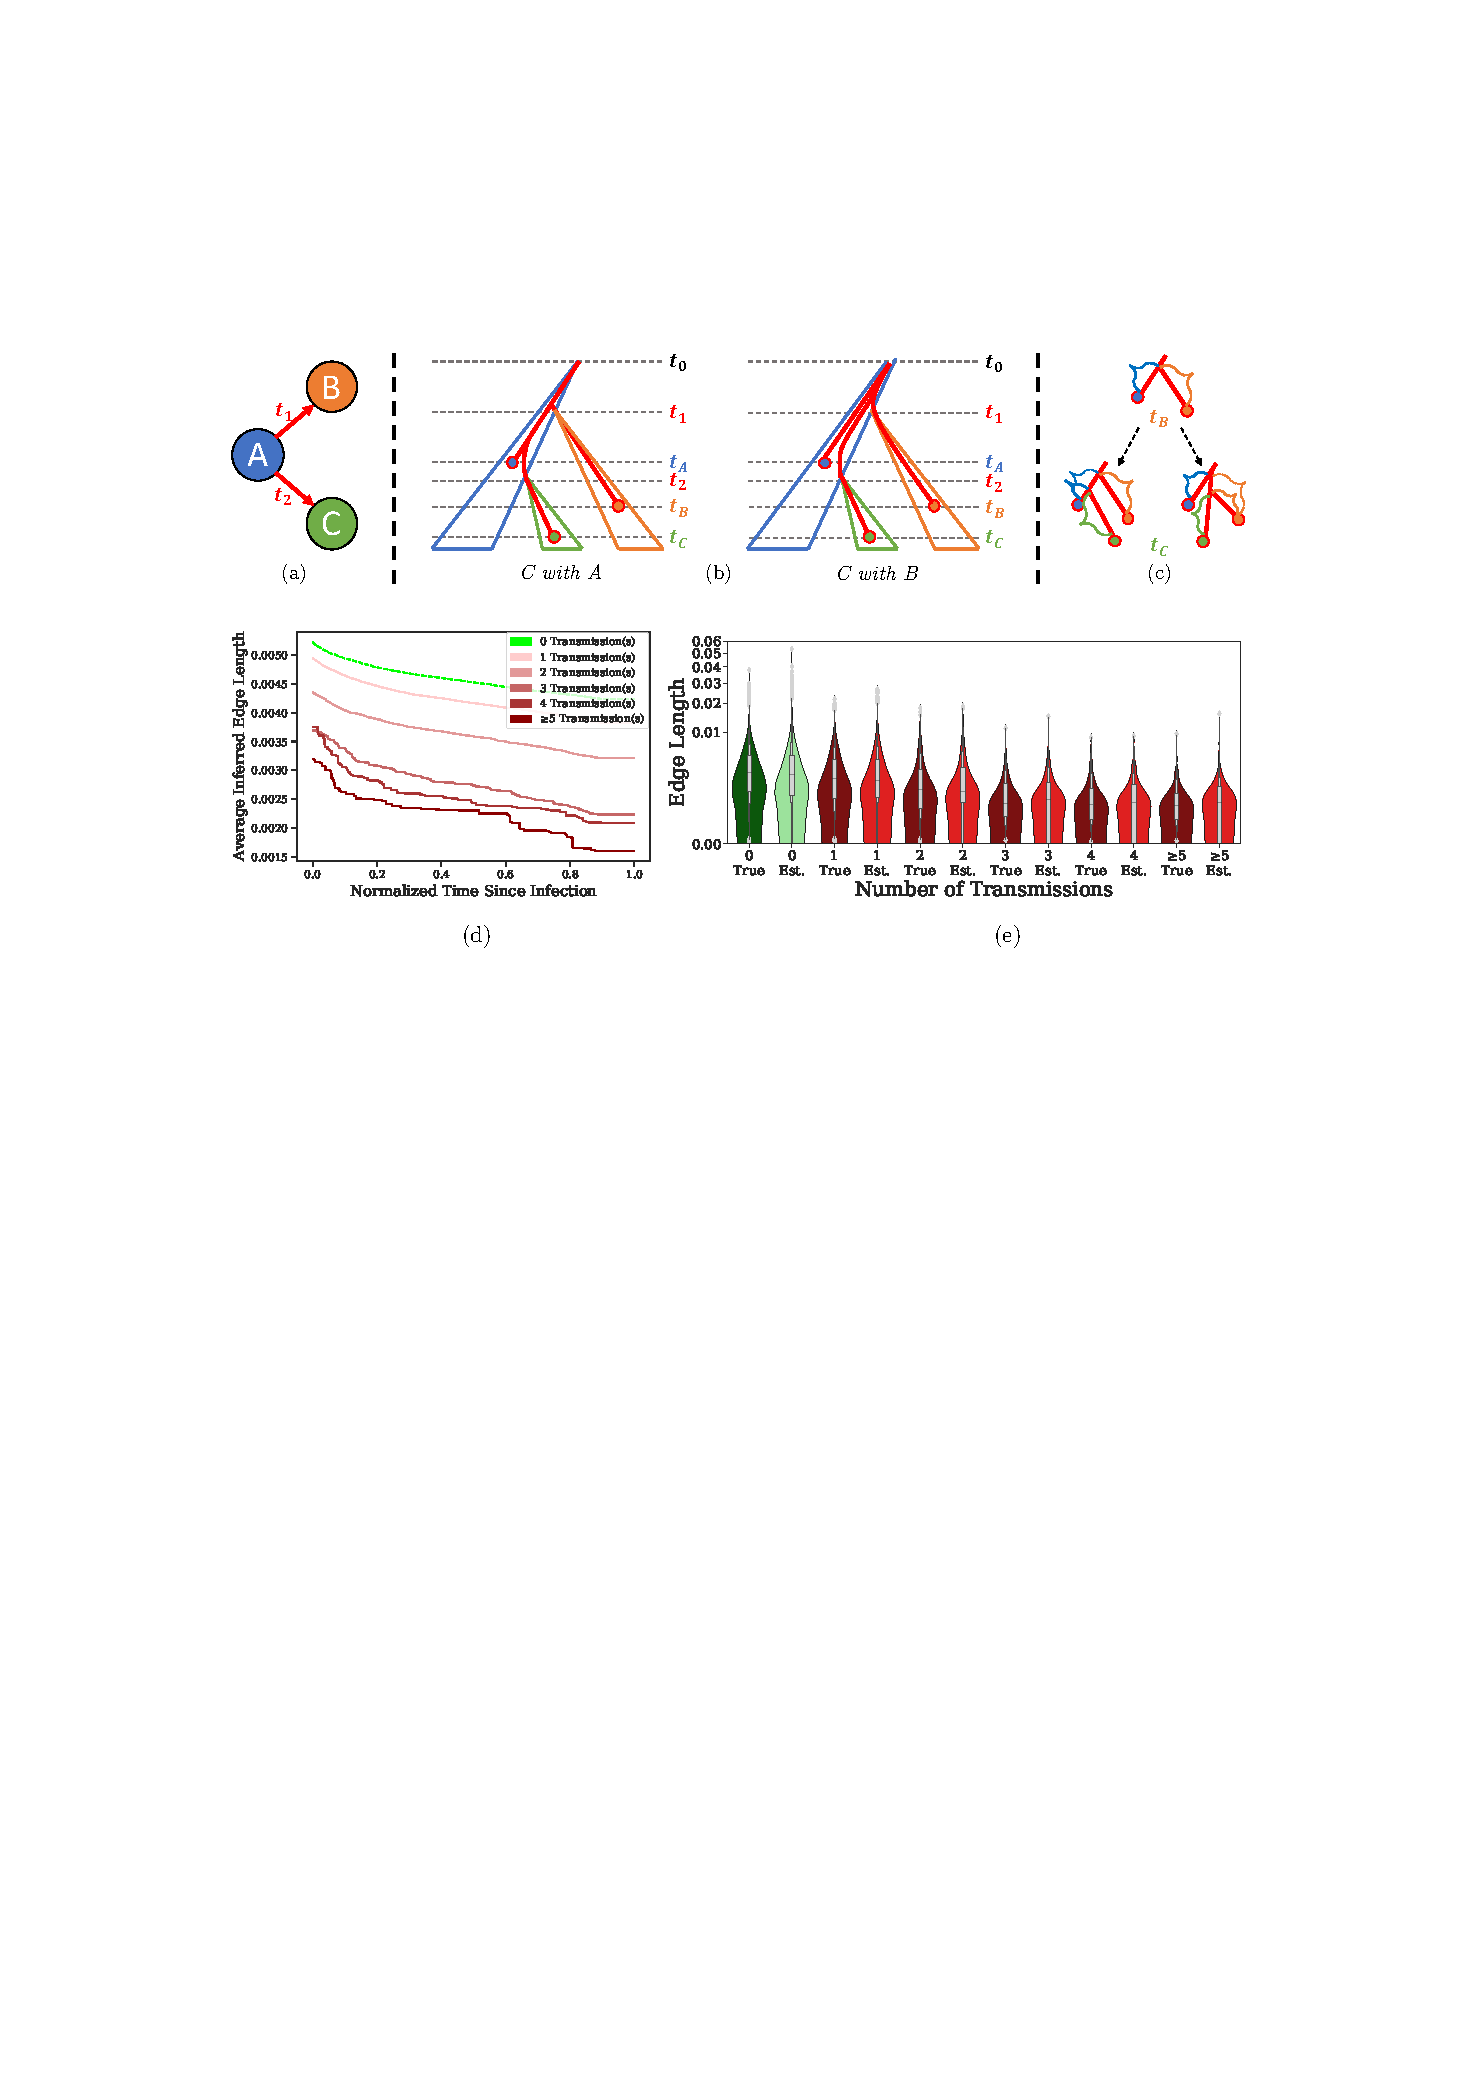
\includegraphics[width=\textwidth]{figs/proact-diagram}
\caption[ProACT Diagram]
{The effect of new transmissions on incident branch lengths. (a) Individual $A$ transmits to individual $B$ and $C$ at times at  $t_1$ and $t_2$, respectively. (b) Viral samples are obtained from individuals $A$, $B$, and $C$ at times $t_A$, $t_B$, and $t_C$. The viral phylogeny of samples is constrained by each transmission event's bottleneck, and the most likely phylogeny matches the transmission history (Left), but in the less likely deeper coalescence, it may not match (Right). (c) Moving from the phylogeny observed at time $t_B$ to the phylogeny at time $t_C$, the branch length incident to individual A  shortens upon the addition of individual C  in the likely event that the coalescence of the lineage from $C$ with the lineage from $A$ is more recent than its coalescence with the lineage from $B$ (Left), or the branch length incident to individual A remains constant in the event of a less likely deeper coalescence (Right). Regardless, the length of the branch incident to individual A never increases.
In simulation, we can observe this trend: as time progresses, the incident branch length of each individual tends to decrease, both in true (Fig.~\ref{fig:proact-true-bl-vs-time}) and inferred (d) phylogenies, and as the number of transmissions from a given individual increases, the distribution of incident edge length tends to decrease, both in true and inferred phylogenies, labeled ``True'' and ``Est.,'' respectively (e).}
\label{fig:proact-diagram}
\end{figure}

\subsection{Motivating the Approach}
We start with the observation that, in simulations (described in detail below), when a phylogeny is inferred from sequences obtained at a given time point in an epidemic,
the more a node transmits, the shorter its incident branch length tends to be (Figs.~\ref{fig:proact-diagram}d--e and~\ref{fig:proact-trans-vs-bl}). Using the Kendall's tau-b test~\cite{Kendall1938}, in a ten-year epidemic simulation (details described below), we found a statistically significant anticorrelation between the incident branch lengths of individuals sampled within the first 9 years of the epidemic and the number of individuals they infected over the final year of the epidemic. This held for true ($\tau=-0.0431$, $p\ll 10^{-10}$) and inferred ($\tau=-0.0354$, $p\ll 10^{-10}$) phylogenetic trees. Though not obvious, this observation can be explained by the constraints placed upon the viral phylogeny by the transmission history (Fig.~\ref{fig:proact-diagram}a--c).

In the context of \gls{HIV} epidemiology in many advanced countries, \glspl{PLWH} are typically sampled upon beginning \gls{ART}. Let's assume for simplicity that every individual in the given dataset has at some point initiated \gls{ART}, meaning future transmissions by individuals in the dataset must happen only if the source stops \gls{ART} or is otherwise unsuppressed. Given a viral phylogeny containing all known \glspl{PLWH}, if, in the future, individual $u$ in the dataset transmits to individual $v$, there are two possible scenarios regarding the placement of the leaf corresponding to $v$ in the existing (true) phylogeny: (1) $v$ is placed on the edge incident to $u$, so the edge incident to $u$ will shorten, or (2) $v$ is not placed on the edge incident to $u$, so the edge incident to $u$ will remain the same length. Although Scenario 2 is possible, Scenario 1 is far more likely \cite{Romero-Severson2016}, and note that the terminal branch lengths do not increase in either scenario. Thus, as time goes by, the terminal branch can only shorten or stay fixed, and it will most often shorten because of new transmissions by the \gls{PLWH} associated with that terminal branch. This pattern, easily observed in simulations (Fig.~\ref{fig:proact-diagram}d), leads to shorter branches for \glspl{PLWH} who have transmitted recently.

Note that \glspl{PLWH} who transmit are unsuppressed. The first time they infect others, their terminal branch length is likely to decrease, and further transmissions further decrease their terminal branch lengths (Fig.~\ref{fig:proact-diagram}d). Thus, one expects nodes with smaller incident branch length to be more likely to have transmitted since their sampling time. Moreover, they are also likely to transmit in the near future because they are likely not to be suppressed. The higher probability of a lack of suppression makes them a good candidate for intervention.

\subsection{Formal Description}
ProACT takes as input a \textit{rooted} phylogenetic tree $T$ of viral samples. Let $bl(u)$ denote the incident branch length of node $u$, and assume the incident branch length of the root of $T$ is 0. Let $a(u)$ denote the vector of ancestors of node $u$ (including $u$), where $a(u)_1$ is $u$, $a(u)_2$ is the parent of $u$, $a(u)_3$ is the grandparent of $u$, etc. Let $r(u)$ denote the length of the path from node $u$ to the root of $T$, i.e., $r(u)=\sum_{v\in a(u)}{bl(v)}$. ProACT sorts the leaves of $T$ in ascending order of $bl(a(u)_1)$, with ties broken by $bl(a(u)_2)$, then by $bl(a(u)_3)$, etc. Note that, for two leaves $u$ and $v$, $|a(u)|$ may be less than $|a(v)|$, in which case, for all $|a(u)|<i\le|a(v)|$, $\frac{r(u)}{|a(u)|-1}$ (i.e., average branch length along the path from $u$ to the root of $T$) is compared with $bl(a(v)_i)$ instead. If two nodes are equal in all comparisons, if the user provides sample times, the earlier sample time is given higher priority; otherwise, ties are broken arbitrarily. Because sorting is needed, for a tree with $n$ leaves, assuming branch lengths are fairly unique, the ProACT algorithm runs in $\bigO(n\log n)$ time. Scalable methods exist both for the inferring~\cite{Price2010,Nguyen2015} and rooting~\cite{Mai2017} very large trees.

\section{Results}
We evaluate ProACT on simulated and real data.

\begin{table}[!ht] % TABLE 1 IN ORIGINAL PAPER
\caption[Varied Simulation Parameters]{Varied \gls{HIV} simulation parameters. Values for the base model condition are shown in bold.}
\vspace{-0.25in}
\begin{center}
\begin{tabular}{|c|c|}
\hline
\textbf{Parameter} & \textbf{Values}\\
\hline
\gls{ART} Start Rate ($\lambda_+$, year$^{-1}$) & \textbf{1}, 2, 4\\
\hline
\gls{ART} Stop Rate ($\lambda_-$, year$^{-1}$) & 0.12 (0.25x), 0.24 (0.5x), \textbf{0.48 (1x)}, 0.96 (2x), 1.92 (4x)\\
\hline
Expected Degree $\left(E_d\right)$ & \textbf{10}, 20, 30\\
\hline
\end{tabular}
\end{center}
\label{tab:proact-favites}
\end{table}

\subsection{Simulation Results}
In order to test ProACT's efficacy, we performed a series of simulation experiments in which we used FAVITES~\cite{Moshiri2018} to generate a sexual contact network, transmission network, viral phylogeny, and viral sequences emulating \gls{HIV} transmission in San Diego from 2005 to 2014 (Material and Methods). We have simulated nine model conditions (Table~\ref{tab:proact-favites}) by starting from a base model condition and varying the rate of \gls{ART} initiation $(\lambda_+)$, rate of \gls{ART} termination $(\lambda_-)$, and the expected degree of the sexual network $(E_d)$. We subsequently inferred and rooted a phylogeny of all sequences obtained during the first 9 years of the simulation. Then, ProACT was run on the true and inferred full trees and subsampled trees.

To measure the efficacy of a given prioritization, we compute the \gls{CMA} of the number of infections caused by the top individuals in the prioritization during the tenth year of the simulation (our outcome measure). The higher the \gls{CMA} for the top individuals in a prioritization, the higher the number of future transmissions from these \textit{top} individuals. Sorting individuals by their outcome measure (known to us in simulations) enables us to compute the optimal \gls{CMA} curve. Also, the mean number of transmissions gives us the expected value of the \gls{CMA} for a random prioritization. Across experimental conditions, the maximum and random expectation vary, so to enable proper comparison of \textit{effects of prioritization} across conditions, we also report an adjusted \gls{CMA} normalizing above the random prioritization and over the optimal prioritization (Eq.~\ref{eq:proact-cma}; see Materials and Methods). Thus, for this Adjusted Transmissions/Person metric, 1 indicates the optimal ordering and 0 indicates ordering that is no better than random.

\begin{figure} % FIGURE 2 IN ORIGINAL PAPER
\centering
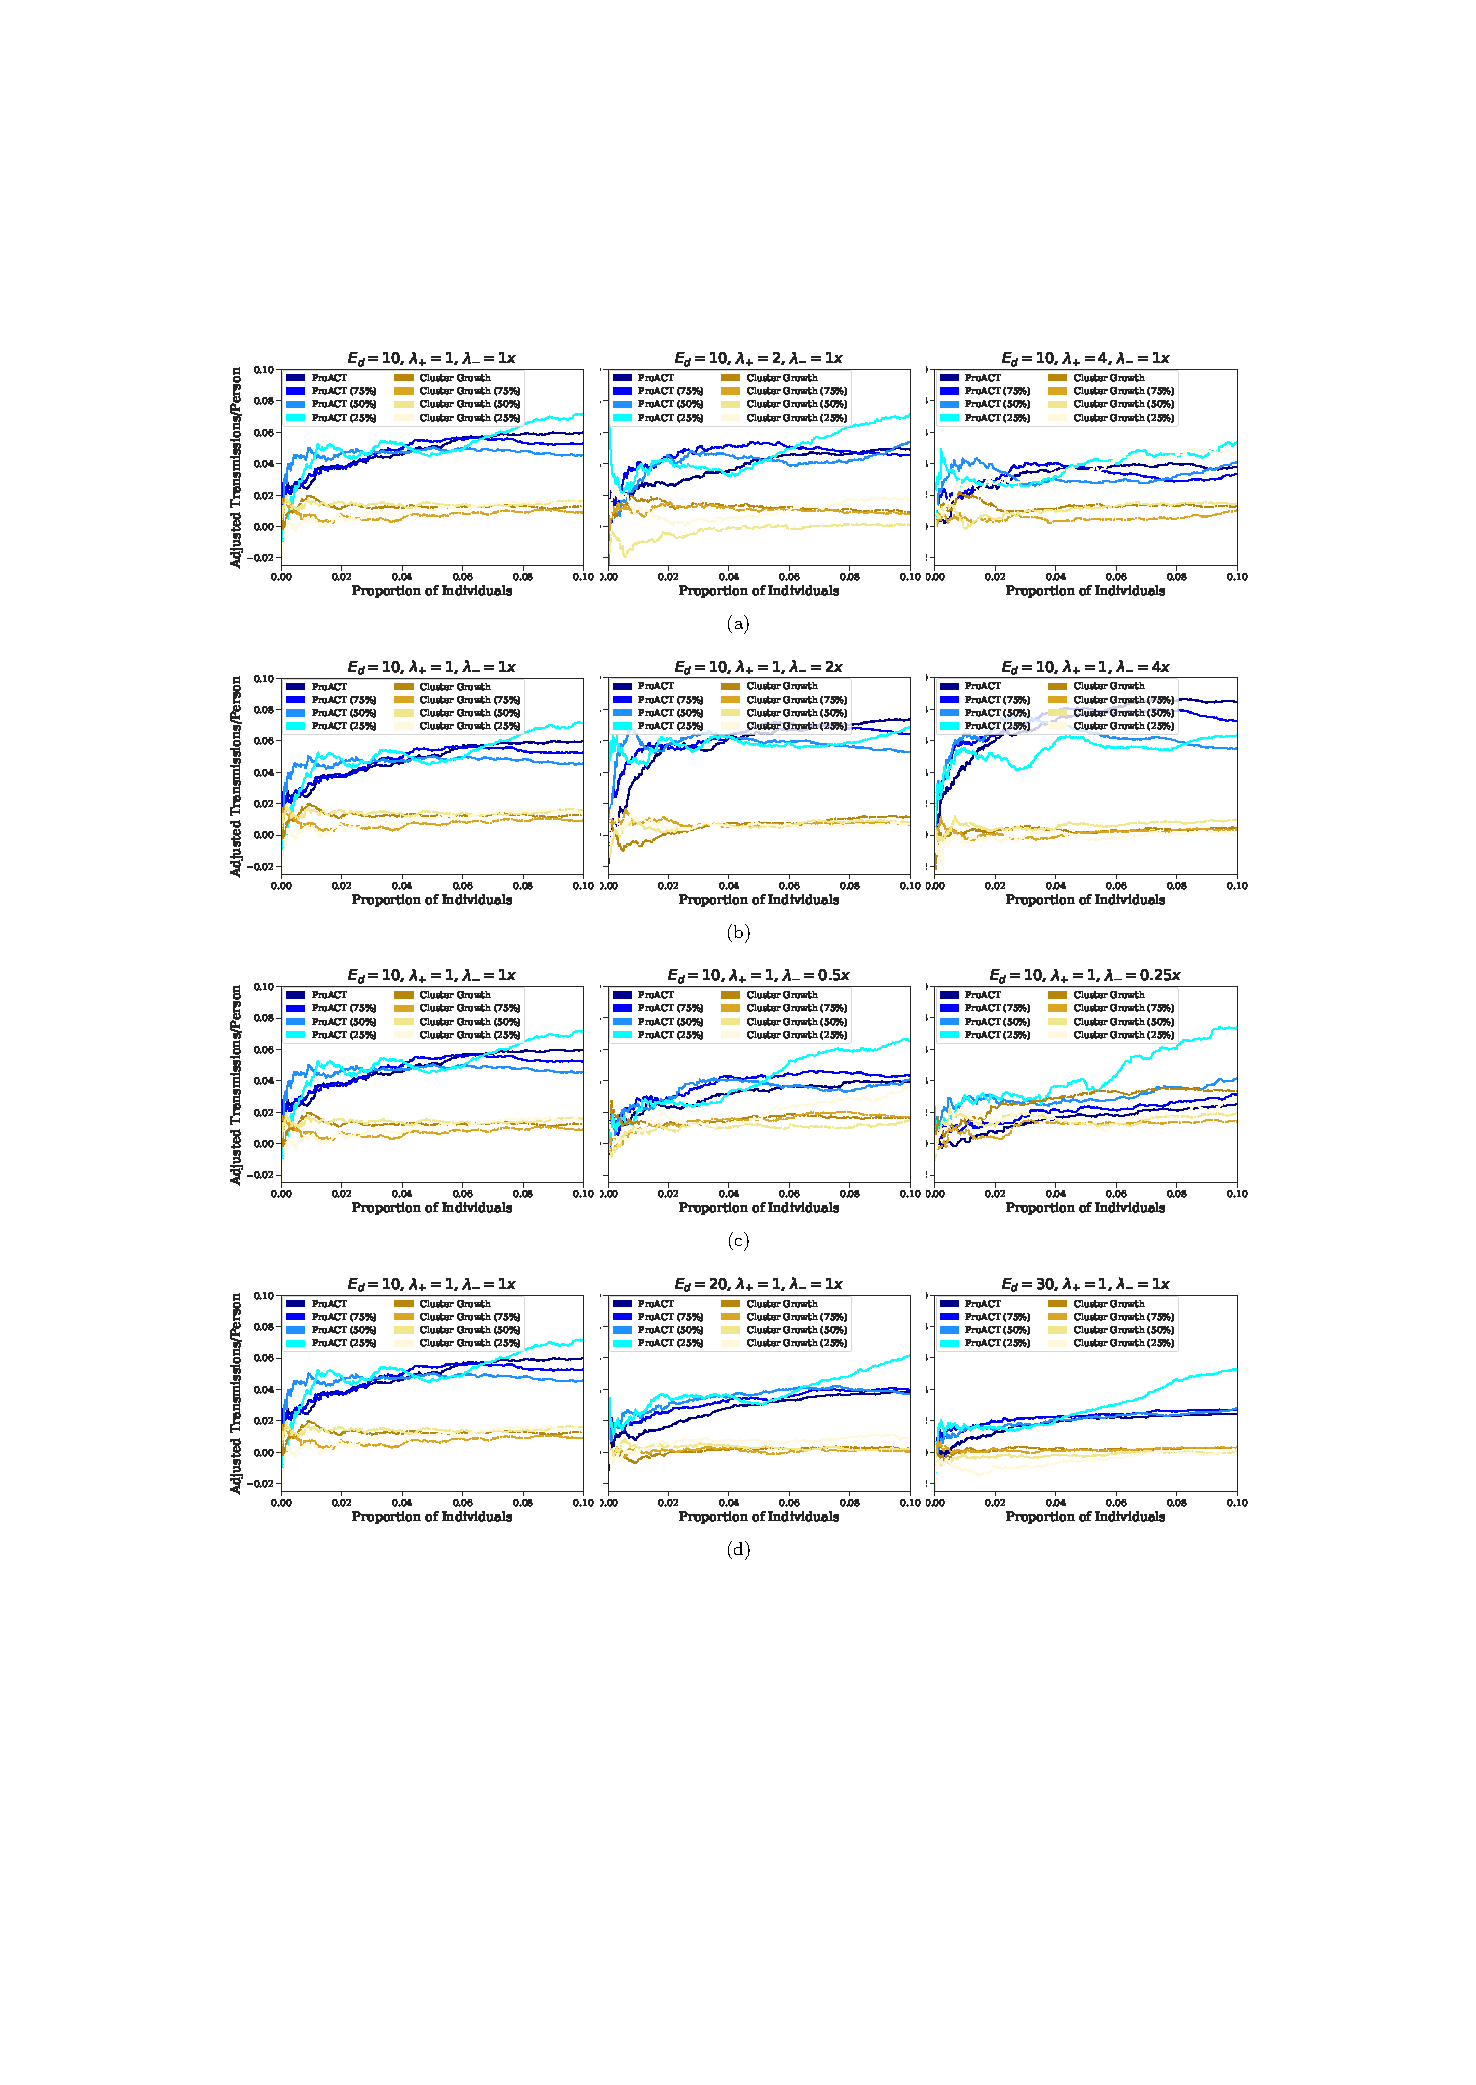
\includegraphics[width=0.77\textwidth]{figs/proact-efficacy}
\caption[Adjusted ProACT Performance on Simulated Datasets]
{ProACT performance on datasets simulated using FAVITES. \gls{CMA} of adjusted number of transmissions per person across the first decile of prioritized \glspl{PLWH} for each simulation parameter set. The horizontal axis depicts the quantile of highest-prioritized \glspl{PLWH} (e.g. $x=0.01$ denotes the top percentile), and the vertical axis depicts their adjusted average number of transmissions per person (1 indicates the optimal ordering, and 0 indicates an ordering that is no better than random). In our simulations, we varied three parameters of interest: (a) the rate of \gls{ART} initiation $(\lambda_+)$, (b-c) the rate of \gls{ART} termination $(\lambda_-)$, and (d) the expected degree of the sexual network $(E_d)$. The simulations were 10 years in length, prioritization was performed 9 years into the simulation, and the adjusted average number of transmissions per person was computed during the last year of the simulation. The curves labeled ``Cluster Growth'' denote prioritization by inferring transmission clusters using HIV-TRACE~\cite{Pond2018} at year 9 of the simulation and sorting clusters in descending order of growth rate since year 8. The curves labeled with percentages denote subsampled datasets. All curves were calculated using 20 simulation replicates.}
\label{fig:proact-efficacy}
\end{figure}

\subsubsection{ProACT Outperforms Random Prioritization Across Conditions}
Across all experimental parameters, ProACT performed much better than one would expect from a random ordering (Fig.~\ref{fig:proact-efficacy}). As we increased the proportion of top individuals selected, ProACT's \gls{CMA} initially increased (e.g. for up to 7\% top individuals in the base model condition) and subsequently flattened out. The most clear signal for benefits of prioritization (e.g, a high \gls{CMA}) is obtained for up to 10\% top-priority individuals (though exact values depend on the model condition).  As the number of selected individuals increases beyond 10\%, however, because the metric of efficacy is \gls{CMA}, the efficacy of a selection will eventually converge towards the efficacy of a random selection by definition (Fig.~\ref{fig:proact-efficacy-wide}).

\subsubsection{ProACT Outperforms Cluster Growth}
As mentioned, Wertheim \textit{et al}. (2018) present a method for prioritizing \glspl{PLWH} by clustering individuals based on viral genetic distance, tracking the size of each cluster over time, and prioritizing clusters in descending order of the growth rate~\cite{Wertheim2018}. The approach can be easily extended to also order individuals (i.e., individuals belonging to clusters with high growth rates are prioritized higher; see Materials and Methods for details). ProACT consistently outperformed prioritization using cluster growth for various parameter choices (Figs.~\ref{fig:proact-efficacy}--\ref{fig:proact-efficacy-vs-n}). The only exception was when the rate of stopping \gls{ART} was lowered all the way to 0.25x, which corresponds to expected time of \gls{ART} termination of 8.3 years. In this condition where adherence was at its highest, prioritization by cluster growth outperformed ProACT when using the full dataset.

\subsubsection{Impact of Simulation Parameters}
As the rate of stopping \gls{ART} $\left(\lambda_{-}\right)$ increased (i.e., with lower adherence), the gap between ProACT and cluster growth grows.
For example, the mean number of transmissions per person among the top 1,000 individuals chosen using ProACT and cluster growth were respectively 0.1702 and 0.0745 (a 1.28x improvement) for the condition with $\lambda_-=4$x. 
This 1.28x improvement gradually decreases to  0.95x, 0.78x, 0.31x, and -0.15x as we reduce the rate or ART termination to 2x, 1x, 0.5x, and 0.25x.
As  $\lambda_{-}$ decreased, ProACT's performance compared to optimal ordering tended to decrease, whereas cluster growth's performance compared to optimal ordering tended to increase; however, ProACT continued to outperform cluster growth for all but the $\lambda_-=$0.25X condition (Fig.~\ref{fig:proact-efficacy}b--c).

\begin{figure} % FIGURE 3 IN ORIGINAL PAPER
\centering
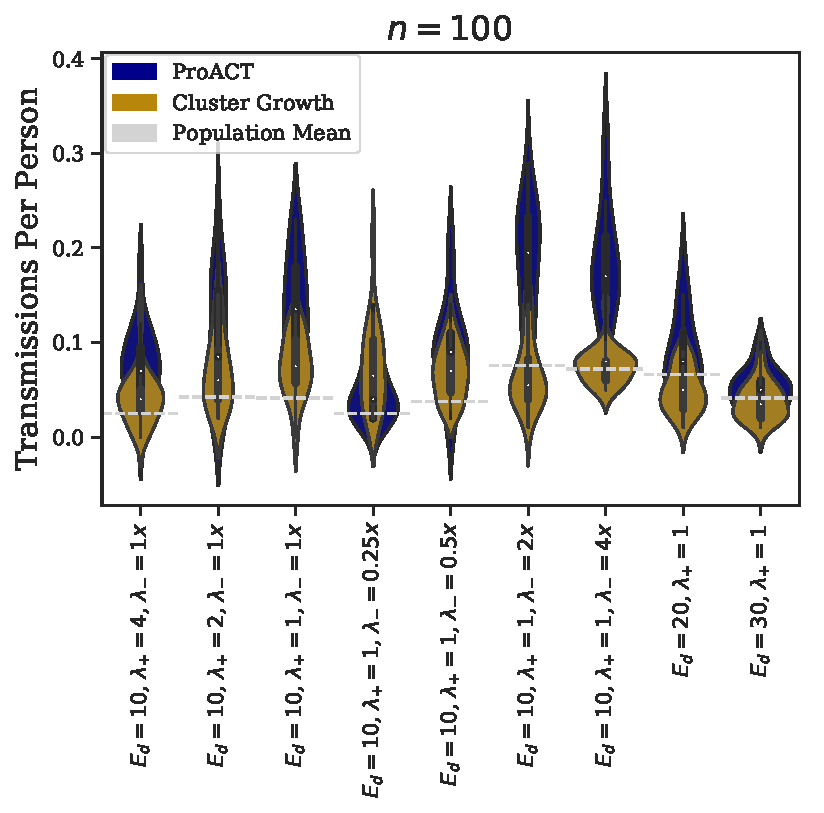
\includegraphics[width=0.495\textwidth]{figs/proact-efficacy-vs-n-100}
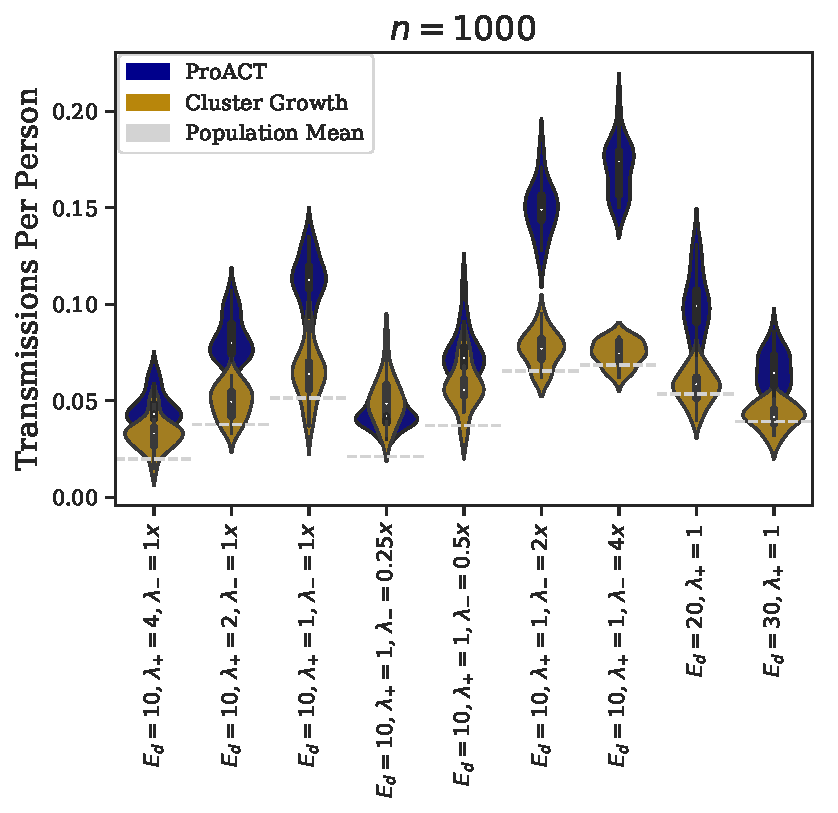
\includegraphics[width=0.495\textwidth]{figs/proact-efficacy-vs-n-1000}
\caption[Raw ProACT Performance vs. Number of Individuals]
{Efficacy on datasets simulated using FAVITES. Average of the raw number of transmissions per person for the top $n$ individuals in a prioritized list vs. simulation parameter set across various values of $n$. The violin plots depicted are across 20 replicates and contain box plots with distribution medians shown as white dots and distribution means shown as dashed grey lines.}
\label{fig:proact-efficacy-vs-n}
\end{figure}

As the rate of starting \gls{ART} $\left(\lambda_{+}\right)$ increased (i.e., with faster diagnoses), the performance of ProACT compared to optimal ordering very slightly degrades (Fig.~\ref{fig:proact-efficacy}a). As a result, the gap between ProACT and cluster growth decreases slightly: when observing the mean number of transmissions per person among the top 1,000 individuals chosen by each method, ProACT experiences a 0.78x, 0.70x, and 0.37x improvement over cluster growth when $\lambda_{+}$ is set to 1x, 2x, and 4x, respectively. Note that as expected, increasing $\lambda_{+}$ reduced the raw number of new infections caused per capita (Fig.~\ref{fig:proact-efficacy-raw}) overall and among top-priority individuals (Fig.~\ref{fig:proact-efficacy-vs-n}).

Effects of the expected number of sexual contacts per person $\left(E_d\right)$, which controls the speed of spread is also interesting (Figs.~\ref{fig:proact-efficacy}d and \ref{fig:proact-efficacy-vs-n}). As $E_d$ increased, the efficacy of both approaches decreased, but ProACT continued to consistently perform many times better than cluster growth.

\subsubsection{Impact of Incomplete Sampling}
Subsampling the total dataset to include $\sfrac{3}{4}$, $\sfrac{1}{2}$, or $\sfrac{1}{4}$ of the total population of \glspl{PLWH} did not have a major impact on the performance of ProACT compared to the optimal ordering (Fig.~\ref{fig:proact-efficacy}). Inevitably, the raw number of new infections decreased as the dataset was subsampled (Fig.~\ref{fig:proact-efficacy-raw}).  However, what remained relatively constant was the benefit of ProACT and cluster growth with respect to optimal and random ordering (e.g. the adjusted metric).

Despite the general robustness, some interesting effects were observed. With $\lambda_{+}=2$x, ProACT's performance remained quite similar across all levels of subsampling, whereas prioritization by cluster growth was negatively impacted by less sampling, especially at the $\sfrac{1}{4}$ level (Fig.~\ref{fig:proact-efficacy}a). Interestingly, for  $\lambda_{-}<1$x, ProACT's performance on  $\sfrac{1}{4}$ sampled datasets \textit{improved} relative to more complete sampling. However, the efficacy of prioritization by cluster growth remained fairly consistent  for  $\lambda_{-}<1$x (Fig.~\ref{fig:proact-efficacy}b--c). Similarly, the performance of ProACT compared to optimal ordering improved with $\sfrac{1}{4}$ sampled datasets when sexual contact degree increased to $E_d\geq 20$ (Fig.~\ref{fig:proact-efficacy}d).

\subsection{Real San Diego Dataset}
We next analyzed a dataset of 926 \gls{HIV}-1 subtype B \gls{pol} sequences obtained in San Diego between 1996 and 2018. To evaluate ProACT accuracy, we divided the data into deciles, with each decile defining two sets: \textit{past} (sequences up to the decile) and \textit{future} (sequences after the decile). We inferred a phylogeny from the sequences present in the \textit{past} set using FastTree~2~\cite{Price2010}, and we used ProACT to order all \glspl{PLWH} in this set. We then evaluated how the outcome measure correlates with the position of each individual in the ordering. We quantify the correlation using Kendall's tau-b, a rank correlation coefficient adjusted for ties~\cite{Kendall1938}. Values range between -1 and 1, with -1 signifying perfect inversion, 1 signifying perfect agreement, and 0 signifying the absence of association.

\begin{figure} % FIGURE 4 IN ORIGINAL PAPER
\centering
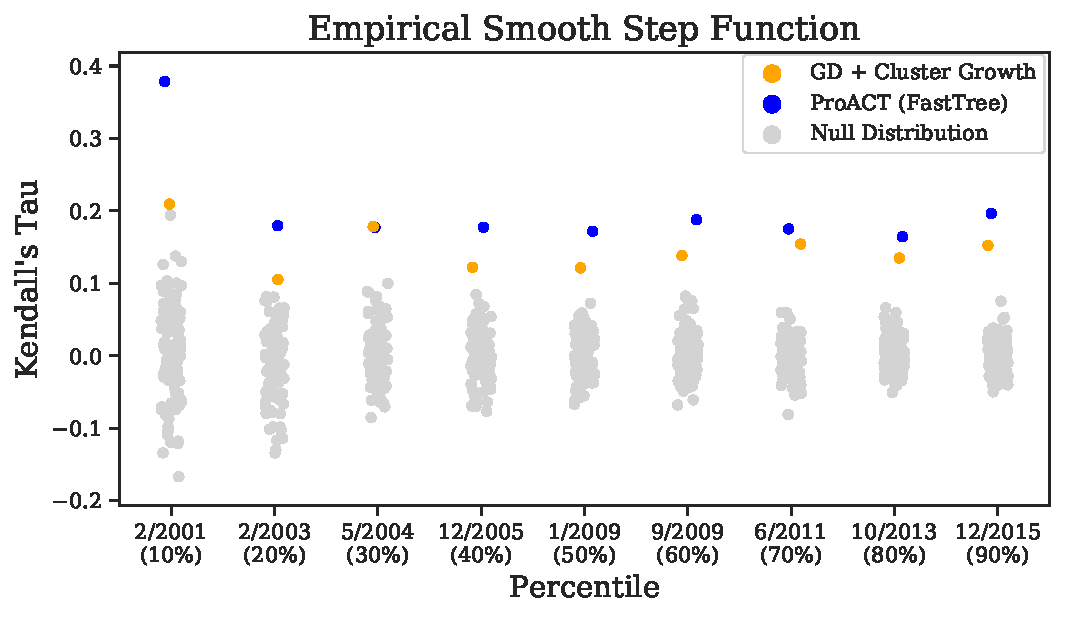
\includegraphics[width=0.495\textwidth]{figs/proact-tautest-smooth}
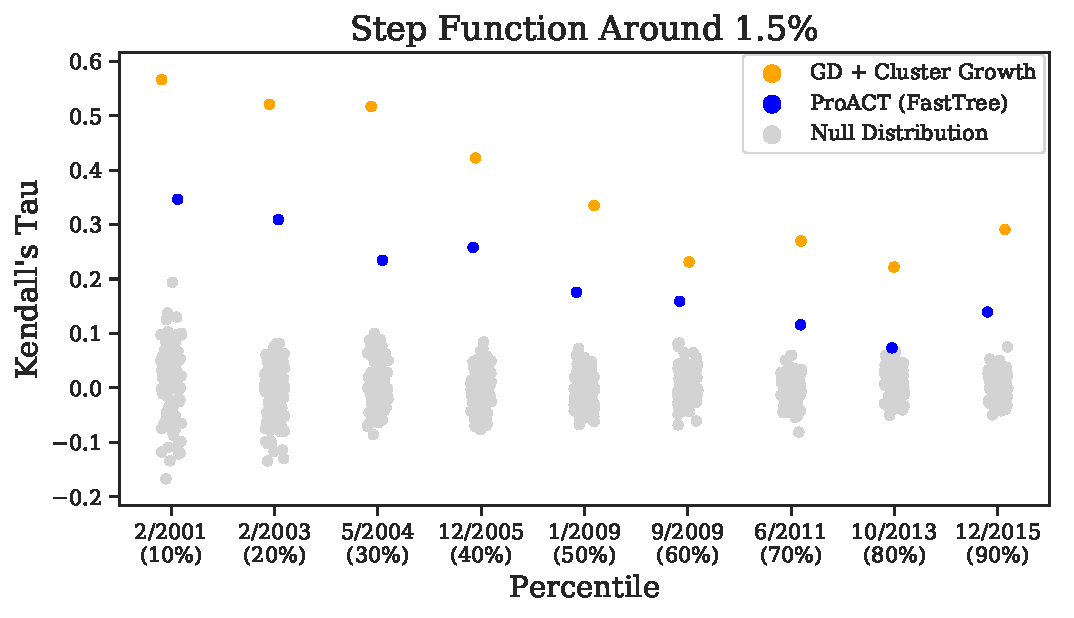
\includegraphics[width=0.495\textwidth]{figs/proact-tautest-strict}
\caption[Kendall's Tau-b Test \textit{p}-Values (Step Functions)]
{Kendall's tau-b test results for ProACT ordering on real data using two riskiness score functions: an empirical smooth step function and a strict step function around 1.5\%. The full San Diego dataset was split into two sets (\textit{pre} and \textit{post}) at each decile (shown on the horizontal axis). The individuals in \textit{pre} were ordered using ProACT and by cluster growth, and they were given a riskiness ``score'' computed using a riskiness score function (see Materials and Methods). Kendall's tau-b correlation coefficient was computed for each ordering with respect to the optimal possible ordering (i.e., sorting in descending order of riskiness score). The null distribution was visualized by randomly shuffling the individuals in \textit{pre}, and test \textit{p}-values are shown in Table~\ref{tab:proact-tautest}.}
\label{fig:proact-tautest}
\end{figure}

On real datasets, unlike the simulated data, the desired outcome measure, the number of new transmissions per person, is not known. Instead, we have to use inferred relationships. HIV-TRACE (used in our cluster growth approach) defines a pair of \glspl{PLWH} as ``genetically linked'' if their sequences are very similar (\gls{TN93} distance below 1.5\%). We similarly use the \gls{TN93} sequence similarity as an outcome measure, but in addition to using a fixed threshold, we also use smoother functions (Fig.~\ref{fig:proact-scorefuncs}). We measure the number of linked individuals using a step function (1 if \gls{TN93} distance is below 1.5\% and 0 otherwise) and an empirical smooth step function determined by fitting a mixture of three Gaussians to the distribution of pairwise \gls{TN93} distances (Material and Methods). We also explore an analytical smooth step function (parameterized sigmoid). Note that, when the step function is used, our outcome measure (computed for future transmissions) is exactly the same as what the cluster growth method uses for prioritizing (albeit, using past data). Thus, it is reasonable to expect the step function will favor cluster growth. As we move to smoother functions of distance to count genetic links, our measure is expected to become less biased in favor of HIV-TRACE.

\begin{table}[!ht] % TABLE 2 IN ORIGINAL PAPER
\caption[Kendall's Tau-b Test \textit{p}-Values (Step Functions)]{Kendall's tau-b test for a null hypothesis that a given prioritization yields a total outcome measure no better than random. We show \textit{p}-values for the real San Diego dataset for the first through ninth deciles using two outcome measure functions. Tests that failed to reject the null hypothesis with (uncorrected) \textit{p}-value $< 0.00138$ (corresponding to $\alpha=0.05$ with a Bonferroni multiple hypothesis testing correct with $n=36$) are marked with \dag.}
\vspace{-0.25in}
\begin{center}
Empirical Smooth Step Function\\
\begin{tabular}{|c|c|c|}
\hline
\textbf{Percentile} & \textbf{GD + Cluster Growth} & \textbf{ProACT (FastTree)}\\
\hline
10\% & $^\dag2\times10^{-3}$ & $^{\ }5\times10^{-8}$\\
\hline
20\% & $^\dag2\times10^{-2}$ & $^{\ }1\times10^{-4}$\\
\hline
30\% & $^{\ }5\times10^{-6}$ & $^{\ }6\times10^{-6}$\\
\hline
40\% & $^{\ }2\times10^{-4}$ & $^{\ }2\times10^{-7}$\\
\hline
50\% & $^{\ }5\times10^{-5}$ & $^{\ }2\times10^{-8}$\\
\hline
60\% & $^{\ }6\times10^{-7}$ & $^{\ }2\times10^{-11}$\\
\hline
70\% & $^{\ }2\times10^{-9}$ & $^{\ }1\times10^{-11}$\\
\hline
80\% & $^{\ }2\times10^{-8}$ & $^{\ }1\times10^{-11}$\\
\hline
90\% & $^{\ }2\times10^{-11}$ & $^{\ }1\times10^{-17}$\\
\hline
\end{tabular}
~\\~\\
Step Function Around 1.5\%\\
\begin{tabular}{|c|c|c|}
\hline
\textbf{Percentile} & \textbf{GD + Cluster Growth} & \textbf{ProACT (FastTree)}\\
\hline
10\% & $^{\ }4\times10^{-12}$ & $^{\ }1\times10^{-5}$\\
\hline
20\% & $^{\ }1\times10^{-19}$ & $^{\ }5\times10^{-8}$\\
\hline
30\% & $^{\ }3\times10^{-28}$ & $^{\ }3\times10^{-7}$\\
\hline
40\% & $^{\ }7\times10^{-25}$ & $^{\ }2\times10^{-10}$\\
\hline
50\% & $^{\ }2\times10^{-19}$ & $^{\ }1\times10^{-6}$\\
\hline
60\% & $^{\ }8\times10^{-12}$ & $^{\ }1\times10^{-6}$\\
\hline
70\% & $^{\ }1\times10^{-17}$ & $^{\ }1\times10^{-4}$\\
\hline
80\% & $^{\ }5\times10^{-14}$ & $^\dag7\times10^{-3}$\\
\hline
90\% & $^{\ }2\times10^{-25}$ & $^{\ }4\times10^{-7}$\\
\hline
\end{tabular}
\end{center}
\label{tab:proact-tautest}
\end{table}

Using both ProACT and cluster growth to prioritize individuals results in orderings of individuals with positive Kendall's tau-b correlations to the number of future genetic links  regardless of the time (i.e., decile) and the function used to count genetic links (Fig.~\ref{fig:proact-tautest}). These correlations are statistically significant in almost all cases  (Table~\ref{tab:proact-tautest} and Fig.~\ref{fig:proact-tautest}). The correlation coefficient ranges ranges between 0.4 (ProACT; 10\% time) and 0.1 (cluster growth; 20\% time) for empirical function, and between 0.6 (cluster growth; 10\% time) and 0.1 (ProACT; 80\% time) for the step function.

The comparison between ProACT and cluster growth depends on the choice of the function to count links. When counting the number of links using the step function, prioritization by cluster growth consistently outperforms ProACT for all deciles of the dataset. These results are not surprising, given that we count HIV-TRACE links both to prioritize and to evaluate. However, according to the empirical smooth step function learned from the \gls{TN93} distances, ProACT outperforms cluster growth in all except one time point, where they are tied.

To further test whether the smoothness of the link-counting function applied to \gls{TN93} distances is a factor in deciding the relative accuracy of methods, we used a sigmoid function to replace the step function while keeping the inflection point at 1.5\% (Fig.~\ref{fig:proact-scorefuncs}). We observed that as the outcome measure function becomes more smooth, ProACT's performance improves with respect to prioritization by cluster growth (Fig.~\ref{fig:proact-tautest-sup}, Table~\ref{tab:proact-tautest-sup}). Based on the more smooth sigmoid function ($\lambda=5$), ProACT outperforms cluster growth in all but one case where they are tied. Thus, simply counting distances close to 1.5\% as partial links leads to evaluations that favor ProACT.

\begin{figure} % FIGURE 5 IN ORIGINAL PAPER
\centering
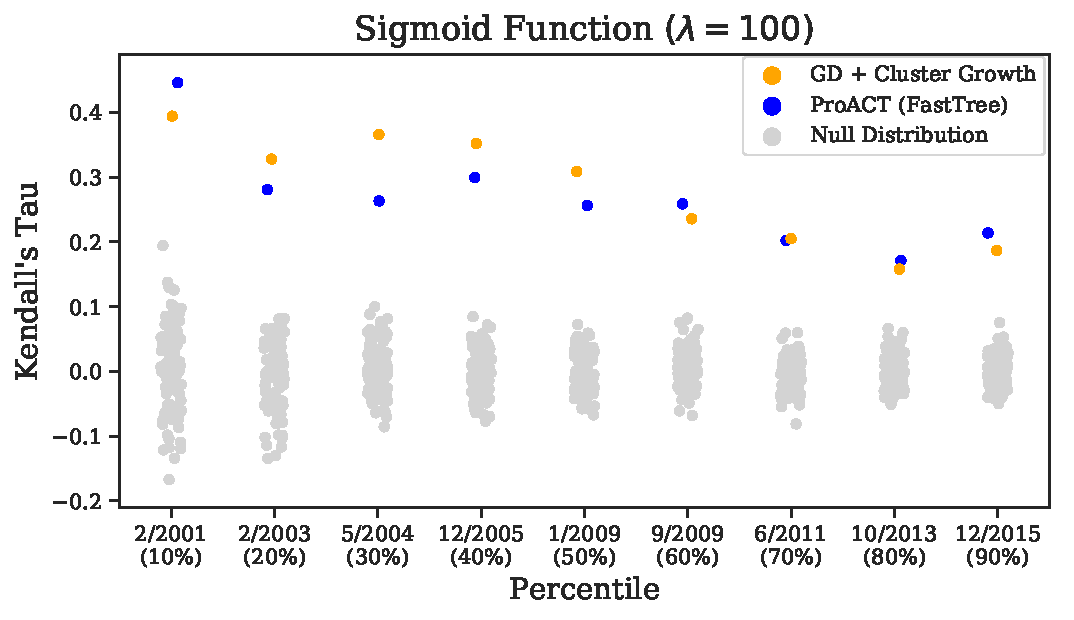
\includegraphics[width=0.495\textwidth]{figs/proact-tautest-L100}
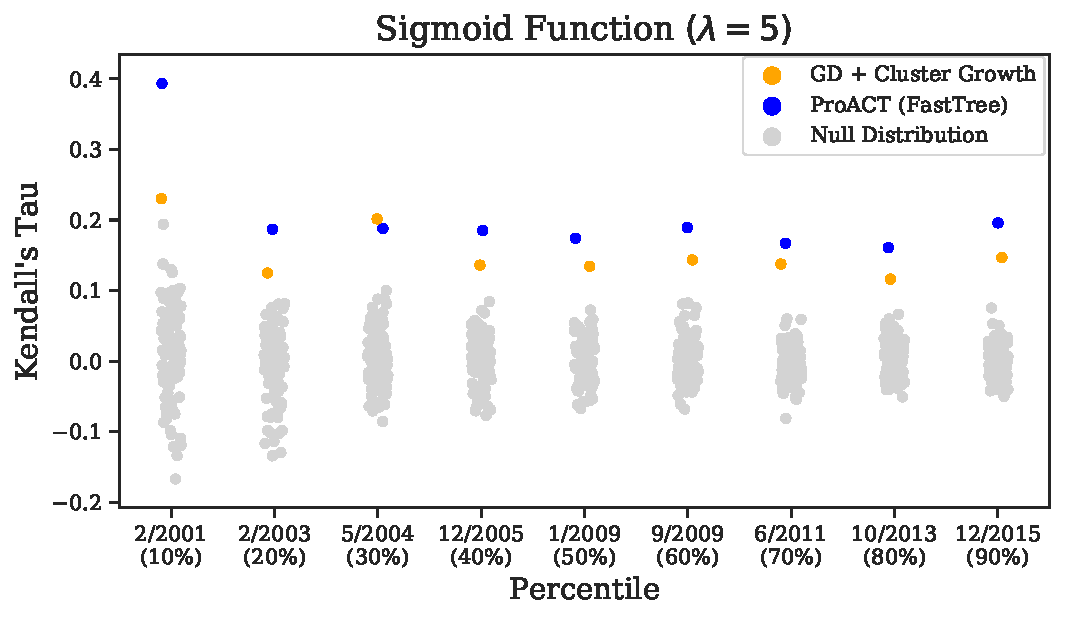
\includegraphics[width=0.495\textwidth]{figs/proact-tautest-L5}
\caption[Kendall's Tau-b Test \textit{p}-Values (Sigmoid Functions)]
{Kendall's tau-b test results for ProACT ordering on real data using the sigmoid riskiness score functions with $\lambda=100$ and $\lambda=5$. The full San Diego dataset was split into two sets (\textit{pre} and \textit{post}) at each decile (shown on the horizontal axis). The individuals in \textit{pre} were ordered using ProACT and by cluster growth, and they were given a riskiness ``score'' computed using a riskiness score function (see Materials and Methods). Kendall's tau-b correlation coefficient was computed for each ordering with respect to the optimal possible ordering (i.e., sorting in descending order of riskiness score). The null distribution was visualized by randomly shuffling the individuals in \textit{pre}, and test \textit{p}-values are shown in Table~\ref{tab:proact-tautest-sup}.}
\label{fig:proact-tautest-sup}
\end{figure}

As time increases, both methods experience seemingly downward trends in their tau coefficients, but the null distribution of tau coefficients also tightens  (Fig.~\ref{fig:proact-tautest}). Thus, both methods consistently do significantly better than expected by random chance and there is no clear relationship between \textit{p}-values of individual tool and time (Table~\ref{tab:proact-tautest}). However, both for the step function and the sigmoid functions, ProACT's relative performance with respect to cluster growth tends to improved over time.

\section{Discussion}
We start by discussing observed results and then comment on practical implications of this paper both for public health and for future research in molecular epidemics. 

\subsection{Discussion of Results}
In our simulations, ProACT was least effective in conditions with very low rate of \gls{ART} termination $(\lambda_{-})$ which correspond to very high adherence. As expected, the total number of new infections originated from \glspl{PLWH} is low when adherence is high (Fig.~\ref{fig:proact-efficacy-raw}) and neither method is much better than random clustering. This observation is consistent with the motivation we presented for the ProACT algorithm. Recall that the motivation relied on identifying \glspl{PLWH} who have stopped being suppressed. If all known \glspl{PLWH} have been started on treatment and none ever stops treatment, prioritization loses its practical relevance, and relatedly, ProACT loses its statistical power. We saw a similar effects when we increased the rate of \gls{ART} $(\lambda_{+})$, which is also not surprising as increasing $\lambda_{+}$ is in effect similar to reducing $\lambda_{-}$.

When we reduced sampling, we did not observe reductions in effectiveness of ProACT and occasionally even observed improvements. These results have to be interpreted in the context of our adjusted metric, which measures benefits over random and below optimal ordering. The per capita number of new infections from high-priority \glspl{PLWH} was \textit{lowered} when we subsampled the datasets (Fig.~\ref{fig:proact-efficacy-raw}). Thus, as expected, when some \glspl{PLWH} are missing from the dataset available to a particular analysis, the overall effectiveness of identifying top priority \glspl{PLWH} reduces. However, the effectiveness reduces equally for the optimal ordering and the ProACT method is not impacted any worse than optimal ordering is. In fact, ProACT is in some cases impacted a bit less harshly than optimal ordering, hence the improvements in adjusted outcome with $\sfrac{1}{4}$ sampling. One should also keep in mind that choosing $x$\% highest priority individuals from the full datasets results in 4x as many individuals as choosing the top $x$\% of the $\sfrac{1}{4}$ subsampled dataset.

The reader is reminded that \glspl{PLWH} are \glspl{PLH} who are also diagnosed, and in our model, are immediately sequenced and put on \gls{ART} (which they may or may not sustain). Thus, \textit{full sampling} refers to a case where all \textit{diagnosed} individuals are included in the dataset and \glspl{PLH} who are not diagnosed are never in our sampling. In other words, the full sampling case should not be misunderstood as including undiagnosed people. Rather, lack of full sampling corresponds to a case where some \glspl{PLWH} are known to \textit{some} clinic but are not included in the study, perhaps due to a lack of sequencing or data sharing.

ProACT far outperformed random ordering and also ordering by cluster growth in simulations. However, we note that, despite the strong performance, there is much room left for future improvement: ProACT consistently ranges in its outcome measure between 2\% and 10\% of the theoretically optimal efficacy when selecting up to 10\% of top-priority \glspl{PLWH}. Thus, there is great room for improvement in identifying high-value individuals compared to our method according to the simulation results. It will be unrealistic to expect that any statistical method based solely on sequence data (and perhaps also commonly available metadata, e.g. sampling times) will be able to come close to the optimal ordering. Nevertheless, it remains likely that methods better than ProACT could in fact be developed.

\subsection{Implications of Results}
In this paper, in addition to introducing ProACT, we formalized a useful approach for thinking about the effectiveness of public health intervention in molecular epidemics. Instead of focusing on the accuracy of methods of reconstructing phylogenetic trees or transmission networks, a question fraught with difficulties, we asked a more practical question. Given molecular epidemic data, can the methods, whether phylogenetic or clustering-based, prioritize \glspl{PLWH} for increased attention by public health? The idea of using molecular epidemics for prioritization is of course not a new idea. For example, as we mentioned, Wertheim \textit{et al}. (2018) presented a method to prioritize \glspl{PLWH} based on the growth rates of their transmission clusters~\cite{Wertheim2018}. Vasylyeva \textit{et al}. (2018) performed a phylogeographic analysis to reconstruct \gls{HIV} movement among different locations in Ukraine in order to infer region-level risk prioritization~\cite{Vasylyeva2018}. Much earlier even, Mellors \textit{et al}. (1996) predicted \gls{HIV} patient prognosis by quantifying \gls{HIV} \gls{RNA} in plasma~\cite{Mellors1996}; predicted prognosis can subsequently be used as a prioritization rank. However, we hope that our formal definition of the problem as a computational question (i.e., prioritization), in addition to our extensive simulations and developed metrics of evaluation will stir further work in this area. As stated before, it seems likely that more advanced methods than our simple prioritization approach can improve performance beyond ProACT in the future.

ProACT prioritizes individuals, not clusters. Prioritizing treatment followup or partner tracing for individuals based on their perceived risk of future transmission promises to be perhaps more effective than targeting clusters. However, such targeted approaches also pose ethical questions that have to be considered. For example, we may not want the algorithm to be biased towards particular demographic attributes. ProACT does not use \textit{any} metadata in its prioritization, reducing risks of such biases. It simply uses the viral phylogeny, which, compared to other types of data, may lead to fewer biases. Nevertheless, it is possible that factors such as the depth of the sampling of a demographic group can in fact change branch length patterns in the phylogeny and make ProACT less or more effective for certain demographic groups. These broader implications of individual prioritization and impacts of demographics on the performance of ProACT should be studied more carefully in future.

One may wonder whether ordering by branch lengths will result in orderings that fail to change with time and reflect the changes in the epidemic. To answer this question, on the San Diego \gls{PIRC} data, we asked how fast the ProACT ordering changes as time progresses. To do so, we computed Kendall's tau-b correlations to the ProACT ordering obtained using only the first decile of the dataset (Fig.~\ref{fig:proact-tautest-first-proact}). There was a strong but diminishing correlation with the initial ordering. The correlations started at 1 (as expected) and gradually decreased in the ninth decile to 0.522. The results show that as desired, ProACT orders do in fact change with time, albeit gradually. The gradual change implies that certain individuals remain high-priority as time progresses. In practical use, ProACT ordering should be combined with clinical knowledge about the status of individual patients. For example, high priority individuals according to ProACT can be given lower priority if they manage to constantly remain suppressed with multiple followups. More broadly, the ProACT ordering should be considered one more tool for prioritizing clinical care, but valuable clinical knowledge, not incorporated into the algorithm, should also be exploited.

Finally, a question faced by public health officials is whether the cost of targeting diagnosed individuals for followups and partner tracing is worth the reduction in future cases. The answer to that question will inevitably depend on who is targeted. For example, in our default simulation case, targeting individuals randomly would at most reduce 0.0529 transmissions per chosen person in the next 12 months, whereas targeting top 1000 individuals according to ProACT would at most reduce 0.119 transmissions. Thus, prioritization can in fact change the cost-benefit analyses. Moreover, given a prioritization, one can use simulations to predict the outcome measure for the top $x$ individuals (similar to Fig.~\ref{fig:proact-efficacy}) and use metrics such as \gls{QALY} to estimate how many top individuals should be targeted for the cost to justify the benefits.

\section{Materials and Methods}
\subsection{Simulated Datasets}
We used FAVITES to simulate a sexual contact network, transmission network, viral phylogeny, and viral sequences emulating \gls{HIV} transmission in San Diego from 2005 to 2014~\cite{Moshiri2018}.

Transmissions were modeled using a compartmental epidemiological model with 5 states: Susceptible (S), Acute \gls{HIV} Untreated (AU), Acute \gls{HIV} Treated (AT), Chronic \gls{HIV} Untreated (CU), and Chronic \gls{HIV} Treated (CT). Individuals in state S (i.e., uninfected) can only transition to state AU. Each infected state $x\in\{\text{AU},\text{AT},\text{CU},\text{CT}\}$ defines a ``rate of infectiousness'' $\lambda_{\text{S},x}$: given an uninfected individual $u$ in state S who has $n_x$ sexual partners in state $x\in\{\text{AU},\text{AT},\text{CU},\text{CT}\}$, the transition of $u$ from S to AU is a Poisson process with rate $\lambda_u=\sum_{x\in\{\text{AU},\text{AT},\text{CU},\text{CT}\}}{n_{x}\lambda_{\text{S},x}}$. To mimic reality, where ART significantly reduces the risk of transmission, rates are chosen such that $\lambda_{\text{S},\text{AU}} > \lambda_{\text{S},\text{CU}} > \lambda_{\text{S},\text{AT}} > \lambda_{\text{S},\text{CT}} \approx 0$. At the beginning of the epidemic simulation, all initially uninfected individuals are placed in state S, and all initially infected (i.e., ``seed'') individuals are distributed among the 4 infected states according to their steady-state proportions. This model is a simplified version of the model proposed by Granich \textit{et al}. (2009)~\cite{Granich2009}.

For the most part, we used the base parameters used in Moshiri \textit{et al}. (2018) that sought to model San Diego~\cite{Moshiri2018}, with the following modifications to better capture reality. See Table~\ref{tab:proact-config-file} for the full set of parameters of the default condition.

\paragraph{Sexual Contact Network.} To capture the scale-free nature of the sexual contact network, Moshiri \textit{et al}. (2018) used the \gls{BA} model~\cite{Barabasi1999}. In addition to the scale-free property, in \gls{HIV} sexual networks, we typically observe many densely-connected communities~\cite{Rothenberg1998}, a property the \gls{BA} model fails to directly model. To have control over the number of communities,  we simulated sexual contact networks such that networks contained 20 \gls{BA} communities, each with 5,000 individuals. In the base condition, the expected degree of connection between an individual and somebody \textit{within} their community was chosen to be 10, and the expected degree between an individual and somebody \textit{outside} their community was chosen to be 1. Each community was simulated separately using the \gls{BA} model and connections between communities were chosen uniformly at random, akin to the \gls{ER} model~\cite{Erdos1959}. Estimates from the literature put the number of contacts at 3--4 during a single year~\cite{Rosenberg2011}. Because our simulated sexual contacts remain static over the 10 year simulation period, we explore mean degrees between 10 and 30.

\paragraph{Epidemic Initialization.} In Moshiri \textit{et al}. (2018), at the start of the epidemic, all infected individuals were in state AU~\cite{Moshiri2018}. Here, instead, we randomly distribute initially infected individuals according to expected proportions of the states. To find these proportions, we ran simulations in which all seed individuals were in state AU, and we observed the proportion of individuals in each state over time, which reached a steady-state fairly early in the simulations (Fig.~\ref{fig:proact-prop-state-vs-time}).

\paragraph{Time of Sequencing.} In Moshiri \textit{et al}. (2018), viral sequences are obtained from individuals exactly at the end time of the 10-year simulation period~\cite{Moshiri2018}. In reality, however, \gls{HIV} patients are typically sequenced when they first visit a clinic to receive \gls{ART}. Thus, it is expected that the terminal branch lengths of trees simulated in Moshiri \textit{et al}. (2018) are artificially longer than would be expected. Instead, we sample viral sequences from individuals the first time they begin \gls{ART} (i.e., the first time they enter state AT or CT). Our current simulation better captures standards of care in advanced health care systems.

\subsubsection{Simulated Data Analysis}
For each simulated sequence dataset, using FastTree~2~\cite{Price2010}, a phylogenetic tree was inferred under the \gls{GTR}+$\Gamma$ model from the sequences obtained in the first 9 years of the simulation. These trees were then MinVar-rooted using FastRoot~\cite{Mai2017}, and ProACT was run on the resulting trees.

\subsection{San Diego Dataset}
To test ProACT on real data, we used a \gls{MSA} of 926 \gls{HIV}-1 subtype B \gls{pol} sequences from San Diego collected by the UC San Diego \gls{PIRC}. \gls{PIRC} is one of the largest longitudinal cohorts of \glspl{PLWH} in the United States. By design, \gls{PIRC} strives to include acute infections (as much as 40\% of recruited individuals are during acute or early stages of infection). Access to the data was obtained through a proposal submitted to \gls{PIRC}.

A phylogenetic tree was inferred from the \gls{MSA} under the \gls{GTR}+$\Gamma$ model using FastTree~2~\cite{Price2010}, and the resulting tree was MinVar-rooted using FastRoot~\cite{Mai2017}. For each decile, using TreeSwift~\cite{Moshiri2018b}, the full tree was pruned to only contain samples obtained up to the end of that decile. ProACT was run on each of the resulting trees.

\subsection{Evaluation Procedure}
\subsubsection{Simulated Data}
To measure the efficacy of a given ProACT selection, because the true transmission histories are known in simulation, we simply average the number of infections caused by the individuals in the selection in the last year of simulation (i.e, after prioritization) to obtain a raw outcome measure.

Let $A=\{1,\ldots,n\}$ denote the first, \ldots, $n$-th sampled individual in the current time step (years 1--9 in our simulations). For each individual $i$, let $c(i)$ denote the number of individuals directly infected by $i$ in the next time step (year 10 in our simulations). Given any set of individuals $s\subseteq A$, let $C(s)=\frac{1}{|s|}\sum_{i\in s}{c(i)}$ denote the average $c(i)$ for all individuals $i\in s$.

Let $x=(x_1,\ldots,x_n)$ denote an ordering of $A$. The (unadjusted) \gls{CMA} of $x$ up to $i$ is $C\left(\{x_1,\ldots,x_i\}\right)$. Let $o=(o_1,\ldots,o_n)$ denote the ordering of $A$ in which elements are sorted in descending order of $c(i)$ (i.e., the optimal ordering), with ties broken arbitrarily. We defined the adjusted \gls{CMA} of $x$ up to $i$ as
\begin{equation}\label{eq:proact-cma}
    \frac{C\left(\{x_1,\ldots,x_i\}\right)-C(A)}{C\left(\{o_1,\ldots,o_i\}\right)-C(A)}\; .
\end{equation}
We use Equation~\ref{eq:proact-cma} to measure the effectiveness of a selection of the top $i$ individuals from each ordering of all individuals. We explore $i$ for 1 to 10\% of the total number of samples (i.e., $\frac{|A|}{10}$).

\subsubsection{Real Data}
The sequences were sorted in ascending order of sample time and, for each decile, they were split at the decile to form two sets: \textit{pre} and \textit{post}. A phylogenetic tree was inferred from the sequences in \textit{pre} under the \gls{GTR}+$\Gamma$ model using FastTree~2~\cite{Price2010} and MinVar-rooted~\cite{Mai2017}. Using the resulting tree, ProACT ordered the samples. Then, pairwise distances were computed between each sequence in \textit{pre} and each sequence in \textit{post} under the \gls{TN93} model~\cite{Tamura1993} using the \texttt{tn93} tool of HIV-TRACE~\cite{Pond2018}.

A natural function to compute the riskiness score of a given individual $u$ in \textit{pre}, similar to that proposed by Wertheim \textit{et al}. (2018)~\cite{Wertheim2018}, is to simply count the number of individuals in \textit{post} who are genetic links to $u$, i.e., $\sum_{v\in post}{\left[d(u,v)\le1.5\%\right]}$. In other words, the score function is simply a step function with value 1 for all distances less than or equal to 1.5\% and 0 for all other distances. However, the selection of 1.5\% as the distance threshold, despite being common practice in many \gls{HIV} transmission clustering analyses, is somewhat arbitrary, and a step function exactly at this threshold may be overly strict (e.g. should a pairwise distance of 1.51\% be ignored?).

To generalize this notion of scoring links, we utilized three analytical score functions. The first is the aforementioned step function $f_1(d)=\left[d\le1.5\%\right]$. The second is a sigmoid function $f_2(d)=\frac{\lambda+1}{\lambda^{d/0.15}+\lambda}$ with the choice of $\lambda=100$ and $\lambda=5$ (Fig.~\ref{fig:proact-scorefuncs}). The third is an empirical scoring function learnt from the data by fitting a mixture model of three Gaussian random variables onto the distribution of pairwise \gls{TN93} distances $f_3(d)=\frac{p_1(x)}{p_1(x)+p_2(x)+p_3(x)}$, where $p_1(x)$ is the \gls{PDF} of the Gaussian component with smallest mean and $p_2(x)$ and $p_3(x)$ are the remaining Gaussian components (Fig.~\ref{fig:proact-scorefuncs}). Specifically, the three Gaussian fits were parameterized by ($\mu_1=0.0191$, $\sigma_1=0.0103$), ($\mu_2=0.0609$, $\sigma_2=0.0118$), and ($\mu_3=0.118$, $\sigma_3=0.0468$), respectively.

For each of these function, for each decile to define \textit{pre} and \textit{post}, we performed a Kendall's tau-b test to compare the prioritization approaches~\cite{Kendall1938}. To generate a null distribution in Figure~\ref{fig:proact-tautest}, we randomly shuffled the individuals in \textit{pre} repeatedly; note however that the \textit{p}-values reported in Table~\ref{tab:proact-tautest} are the theoretical \textit{p}-values computed by the tau-b test, not empirically estimated from our repeated shuffling.

\section{Acknowledgments}
We thank Susan B. Little for providing the San Diego \gls{HIV} sequence dataset used in this study. We also thank Joel O. Wertheim and Sanjay R. Mehta for fruitful discussions that helped motivate the development of ProACT.

This work was supported by the National Institutes of Health (5P30AI027767-28, AI100665, AI106039, and MH100974) and a developmental grant from the University of California, San Diego Center for AIDS Research (P30 AI036214), supported by the National Institutes of Health.

Chapter~\ref{chap:proact}, in full, has been submitted for publication of the material as it may appear in (2019) Moshiri, Niema; \textit{Molecular Biology and Evolution}. The dissertation author was the primary investigator and first author of this paper.

%% END PROACT CHAPTER
%% START TREESWIFT CHAPTER
\chapter{\treeswifttitle}
\label{chap:treeswift}
\clearpage

Phylogenetic trees are essential to evolutionary biology, and numerous methods exist that attempt to extract phylogenetic information applicable to a wide range of disciplines, such as epidemiology and metagenomics. Currently, the three main Python packages for trees are Bio.Phylo, DendroPy, and the ETE Toolkit, but as dataset sizes grow, parsing and manipulating ultra-large trees becomes impractical for these tools. To address this issue, I developed TreeSwift, a user-friendly and massively scalable Python package for traversing and manipulating trees that is ideal for algorithms performed on ultra-large trees.

\section{Motivation and Significance}\label{sec:treeswift-background}
Phylogenetic trees are essential to evolutionary biology, and phylogenetic methods are applicable to a wide range of disciplines, such as epidemiology \cite{Ragonnet-Cronin2013,Rose2017} and metagenomics \cite{Kembel2011,Darling2014,Filipski2015}. However, the datasets analyzed by these methods are growing rapidly as sequencing costs continue to fall, emphasizing the need for scalable methods of tree traversal and manipulation. Beyond the analysis of real datasets, phylogenetic approaches can be utilized in the analysis of potentially massive datasets generated by simulation experiments~\cite{Moshiri2018}.

Methods for performing phylogenetic analyses such as clustering~\cite{Balaban2019} and rerooting~\cite{Mai2017} are typically presented as a series of higher-level tree traversals and manipulations. The developers of these tools do not commonly implement basic tree processing from scratch: they typically utilize existing tree packages to handle low-level tasks and instead implement their algorithms as a series of calls to functions of these packages. As a result, the performance of such a tool depends not only on the time complexity of its algorithm, but also on the performance of the underlying tree package.

Currently, the three main Python packages for trees are the Bio.Phylo module of Biopython~\cite{Cock2009}, DendroPy~\cite{Sukumaran2010}, and the ETE Toolkit~\cite{Huerta-Cepas2016}. The three tools are simple to integrate into new methods, include a plethora of functions that cater to most phylogenetics needs, and are fast for reasonably-sized trees. However, as dataset sizes grow, parsing and manipulating ultra-large trees becomes impractical. I introduce TreeSwift, a scalable cross-platform Python package for traversing and manipulating trees that does not require any external dependencies, and I compare its performance against that of Bio.Phylo, DendroPy, and the ETE Toolkit.

\section{Software Description}\label{sec:treeswift-description}
\subsection{Software Overview}\label{sec:treeswift-overview}
TreeSwift is a pure-Python package that has no required external dependencies and which has been tested on Python versions 2.6--2.7 and 3.3--3.7. It is also compiled and hosted on PyPI, meaning it can easily be installed with a single \texttt{pip} command without any need for administrative privileges or any advanced knowledge. This is essential to contrast against the current state-of-the-art, ETE Toolkit, which requires the Six and NumPy Python libraries to install if the user has administrative privileges or Anaconda/Miniconda to install if the user doesn't, and BioPython, which requires a C compiler and the NumPy Python library as well as the computer fluency to compile tools from source using a \texttt{Makefile}.

A key feature of TreeSwift is its simplicity in class design in order to reduce time and memory overhead of loading, traversing, and manipulating trees. The entire package consists of just two classes: a \texttt{Node} class, which contains the data and local relationships, and a \texttt{Tree} class, which handles manipulation and traversal on the \texttt{Node} objects. A key distinction between TreeSwift and DendroPy is that DendroPy stores bipartition information to enable efficient comparisons between multiple trees that share the same set of taxa, but because TreeSwift is designed for the fast traversal and manipulation of individual trees (and not for the comparison of multiple trees), TreeSwift forgoes this feature to avoid the accompanied overhead, resulting in a much lower memory footprint and faster execution of equivalent functions (Fig.~\ref{fig:treeswift-comparison}).

\begin{figure} % FIGURE 1 IN ORIGINAL PAPER
\centering
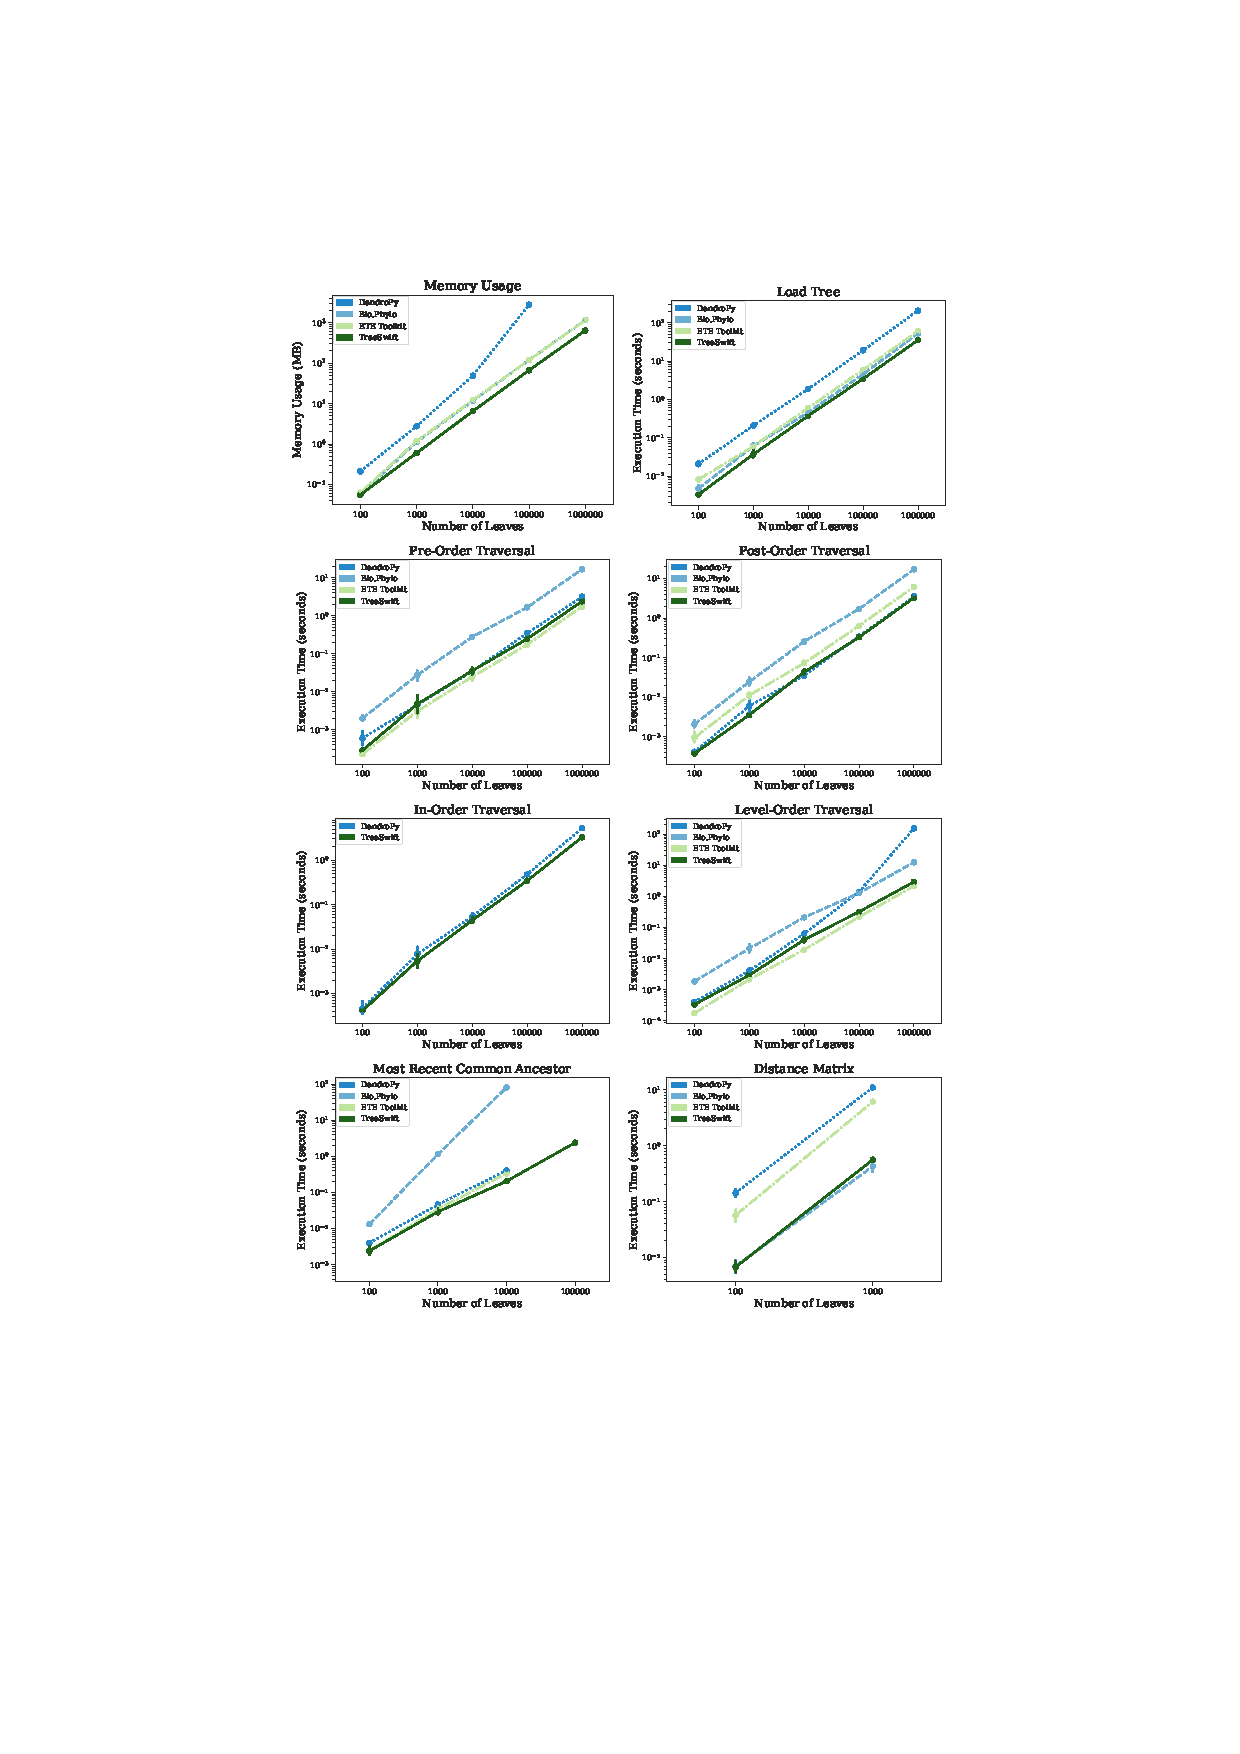
\includegraphics[width=0.7\textwidth]{figs/treeswift-comparison}
\caption[Runtime Comparison]
{Runtimes of DendroPy, Bio.Phylo, the ETE Toolkit, and TreeSwift for a wide range of typical tree operations using trees of various sizes, as well as memory consumption after loading a tree. The truncation of a given tool's plot implies lack of scalability beyond that point, and the entire lack of a given tool implies lack of implementation of the tested functionality. Timing was performed on a computer running CentOS release 6.6 (Final) with an Intel(R) Xeon(R) CPU E5-2670 0 at 2.60GHz and 32 GB of RAM.}
\label{fig:treeswift-comparison}
\end{figure}

\subsection{Software Functionalities}\label{sec:treeswift-functions}
TreeSwift supports loading trees in the Newick, Nexus, and NeXML file formats via the \texttt{read\_tree\_newick}, \texttt{read\_tree\_nexus}, and \texttt{read\_tree\_nexml} functions, respectively. Inputs to these functions can be strings, plaintext files, or gzipped files, and TreeSwift handles the nuances of parsing them internally to maintain user-friendly operability.

TreeSwift provides generators that iterate over the nodes of a given tree in a variety of traversals, including pre-order, in-order, post-order, level-order, and root-distance-order. TreeSwift also allows for the modification of the structure of a given tree by simply modifying the \texttt{Node} objects of the tree. These built-in generators and modifiers intend to provide developers a simple yet efficient manner in which to implement their own algorithms such that they only need to consider higher-level details of the traversal process.

TreeSwift also provides the ability to compute various summarizing statistics of a given tree, such as tree height, average branch length, patristic distances between nodes in the tree, treeness~\cite{Phillips2003}, and the Gamma statistic~\cite{Pybus2000}. Beyond numerical statistics to describe trees, TreeSwift can also generate a visual summary of a tree in the form of a \gls{LTT} plot~\cite{Harvey1994}, a feature not currently implemented in any other Python tree package.

\section{Illustrative Example}\label{sec:treeswift-example}
In the following example, I load a tree from a gzipped file, compute the minimum distance from each node in the tree to a leaf, print the minimum leaf distance of the root, and create a \gls{LTT} plot (Fig.~\ref{fig:treeswift-ltt}).
\clearpage

\begin{python}
from treeswift import read_tree_newick
tree = read_tree_newick("my_huge_tree.nwk.gz")
min_leafdist = dict()
for u in tree.traverse_postorder():
    if u.is_leaf():
        min_leafdist[u] = 0
    else:
        min_leafdist[u] = min(min_leafdist[c]+c.edge_length for c in u.children)
print("Minimum leaf distance from root: %f" % min_leafdist[tree.root])
tree.lineages_through_time(color="blue")
\end{python}

\begin{figure} % FIGURE 2 IN ORIGINAL PAPER
\centering
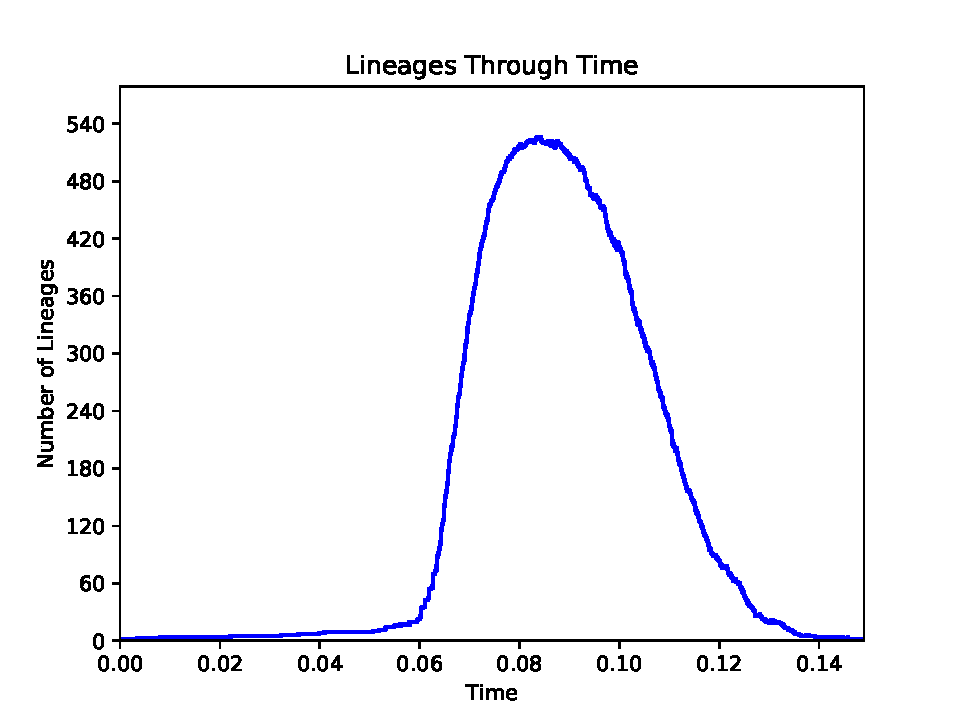
\includegraphics[width=0.7\textwidth]{figs/treeswift-ltt}
\caption[Lineages Through Time]
{Example \gls{LTT} plot generated using TreeSwift.}
\label{fig:treeswift-ltt}
\end{figure}

\section{Impact}\label{sec:treeswift-impact}
The key impact of TreeSwift is its significant performance improvement over existing Python tree packages (Fig.~\ref{fig:treeswift-comparison}). For almost all tested tree operations, TreeSwift performed tasks significantly faster than all existing tools (by orders of magnitude at times), and it was the only tool that not only had all tested functions implemented, but that also was able to scale to the largest of tested datasets. Further, TreeSwift's memory consumption was significantly lower than all existing tools. Thus, phylogenetic tools written in Python can utilize TreeSwift for scalability.

Further, TreeSwift was designed to be simple to use. As can be seen in the example code in Section~\ref{sec:treeswift-example}, a user with minimal Python experience can generate a \gls{LTT} plot in just 3 lines of Python code. Even complex tree algorithms can be implemented cleanly by utilizing TreeSwift's traversal generators \cite{Balaban2019}.

It must be emphasized that, although TreeSwift was designed with the field of phylogenetics in mind, the package is general in that it can be utilized with any arbitrary tree structure, including those in non-phylogenetic applications~\cite{Moshiri2018b}. Thus, its utility can extend well beyond its intended phylogenetics audience.

\section{Conclusions}\label{sec:treeswift-conclusions}
In this article, I presented TreeSwift, a pure-Python package for loading, traversing, and manipulating trees in a massively-scalable manner. The current version implements a wide range of typical tree operations, and due to its simple design, I hope to engage other developers to further expand TreeSwift's capabilities to target a larger suite of potential applications.

\section{Acknowledgements}
This work was supported by NIH subaward 5P30AI027767-28 to NM. I would like to acknowledge Siavash Mirarab for his mentorship. I would also like to acknowledge Jeet Sukumaran and Mark Holder, as DendroPy provided much motivation during TreeSwift's development.

\acktreeswift

%% END TREESWIFT CHAPTER
%% START EDUCATION CHAPTER
\chapter{\educationtitle}
\label{chap:education}
\clearpage

With rapid advances in sequencing technologies, the entire field of biology has largely shifted to depend upon the ability to analyze ultra-large datasets. As a result, the ability to perform basic computation has become a necessary prerequisite for successful biological research, yet it is only barely beginning to enter official undergraduate biology curricula as a required topic. Further, these skills are required not only by undergraduate biologists, but by graduate students, post-docs, and even faculty members and professionals, yet these individuals may not have the ability to enroll in undergraduate Computer Science courses. In an attempt to address this gap in education availability, I have dedicated significant effort to develop \glspl{MAIT} for use in \glspl{MOOC} as well as in flipped in-person classrooms.

\section{Introduction}
\subsection{Bioinformatics Education: The New Frontier}
With the introduction of \gls{NGS} technologies, researchers gained the ability to perform large-scale sequencing experiments at extremely high throughput with relatively low costs~\cite{Metzker2010}. Due to the massive sizes of the datasets that are produced in such experiments, basic computational education has become increasingly necessary for successful biological research. While professors at top universities have started introducing bioinformatics courses into undergraduate curricula in recent years~\cite{Compeau2019,Mulder2018,Madlung2018}, access to such courses is typically restricted to students who have the ability to \textit{enroll} in undergraduate courses at these top universities. However, high tuition costs disproportionately prevent low-income and minority students from entering such universities~\cite{Wetzel1998}, leading to disparity in terms of who actually has access to such learning materials. Further, undergraduate students are not the only audience of interest for courses in such topics: graduate students, post-docs, and even faculty and professionals who received formal training in biological and biomedical sciences without any computational coursework are in need of these bioinformatics courses. In addition to difficulties faced by students, due to the rapid growth of the popularity of computational courses~\cite{Camp2017}, instructors of such courses tend to struggle to scale their courses to accommodate large class sizes.

\subsection{The MOOC Revolution}
With the creation of companies like Coursera and edX, university professors started to develop \glspl{MOOC}: tuition-free courses taught over the internet to a large number of students. What started as just a handful of courses, such as \textit{Machine Learning} by Andrew Ng (2012)~\cite{Ng2012}, eventually blew up, and all major universities started releasing \glspl{MOOC} on a wide range of subjects~\cite{Pappano2012}. Much research went into how to design these courses~\cite{Guardia2013,Bruff2013,Breslow2013,Guo2014}. Further, \glspl{MOOC} seemed to attract increased participation by residents of countries in which higher education is extremely rare, far more significant representation of women than in universities, a large proportion of individuals who are either unemployed or seeking to change field of employment, and a considerable number of individuals simply taking courses for interest~\cite{Bayeck2016}. However, their reception was generally mixed: some enjoyed the freedom of filling their education gaps at their own pace~\cite{Milligan2017}, whereas others were pessimistic about their educational value~\cite{Vardi2012}. Many complaints were aimed at the passive learning encompassed in traditional \glspl{MOOC}, in which students simply watch a series of lecture videos and answer simple multiple choice quizzes embedded throughout.

\subsection{From MOOCs to MAITs}
Phillip Compeau and Pavel Pevzner released the first ever bioinformatics \gls{MOOC}, \textit{Bioinformatics Algorithms} (2014)~\cite{Compeau2014}, and with it, a new technology to revolutionize online learning: the \gls{MAIT}, an online text that has integrated quizzes, numerical problems, and even coding challenges to allow the learner to directly interact with the content and to allow the instructor to enable active learning, even in a remote and automated setting~\cite{Compeau2015}. The challenges are adaptive in that they provide the student uniquely-tailored feedback based on the student's specific misconception, and the text itself is adaptive in that the user can take his or her own unique ``learning path.'' For example, a biology student would have the ability to take optional ``detours'' on prerequisite computer science topics such as time complexity, whereas a computer science student would have the ability to take optional ``detours'' on prerequisite biology topics such as the Central Dogma. These carefully-written \glspl{MAIT} were the foundation upon which the \textit{Bioinformatics Algorithms} \glspl{MOOC} were built, and the adaptivity and interactivity was generally well-received by the learners.

\subsection{``Bioinformatics'' Means Nobody Gets Left Behind}
Despite the great success of the \textit{Bioinformatics Algorithms} \glspl{MOOC}, the space of online bioinformatics education was not yet filled: these courses were excellent for students with extensive backgrounds in programming, discrete mathematics, and algorithms, but for all biologists who wanted to transition into the computational aspects of the field, these courses were incomprehensible due to the students' lack of computational background. This motivated my work in bioinformatics education: the development of beginner-friendly \glspl{MAIT} to embed within \glspl{MOOC} as well as to integrate into offline classrooms.

\section{Methods}
\subsection{Teaching Philosophy}
Just like running a traditional offline classroom, developing a \gls{MAIT} requires the implementation of various pedagogical techniques to optimize the learning experience and to enhance student outcomes. As such, the pedagogical design of a \gls{MAIT} is essential to its success. In this section, I discuss the pedagogical techniques I utilize when developing \glspl{MAIT}.

\subsubsection{Bloom's Taxonomy}
Bloom's Taxonomy is a set of three hierarchical models used to classify educational learning objectives into levels of complexity and specificity~\cite{Bloom1956}. The cognitive (i.e., knowledge-based) domain of the taxonomy is a hierarchy containing the following levels: Remember, Understand, Apply, Analyze, Evaluate, and Create (Fig.~\ref{fig:education-bloom-taxonomy})~\cite{Anderson2001}. I follow the guidelines of Bloom's Taxonomy when developing my materials.

\begin{figure}
\centering
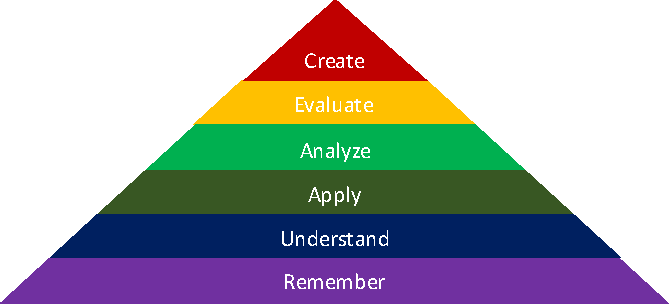
\includegraphics[width=0.65\textwidth]{figs/education-bloom-taxonomy}
\caption[Bloom's Taxonomy]
{Bloom's Taxonomy}
\label{fig:education-bloom-taxonomy}
\end{figure}

\subsubsection{Active Learning}
Within my \glspl{MAIT}, I implement the Active Learning approach: students actively engage with the materials as opposed to simply passively reading or viewing them~\cite{Bonwell1991}. Specifically, I integrate numerous multiple choice, short answer, numerical, and coding challenges that can be solved directly within the text. By undergoing frequent assessment throughout the learning process, students are able to gauge their mastery of concepts \textit{throughout} a given section, and they will be able to correct their misconceptions precisely when they occur (unlike many existing self-paced learning resources, which typically assess student mastery at the \textit{end} of each section).

\subsubsection{Adaptive Learning}
A common misconception is that online education lacks the personalized qualities of an offline course. However, on the contrary, in my \glspl{MAIT}, I demonstrate that my tens of thousands of students are able to receive far more personalized feedback than is possible in an offline class of even tens of students. Specifically, in my \glspl{MAIT}, all challenges (including coding) are automatically graded via carefully-designed \glspl{ITS}, which attempt to provide students uniquely-tailored feedback based on their specific misconceptions (Fig.~\ref{fig:education-code-challenge}).

\begin{figure}
\centering
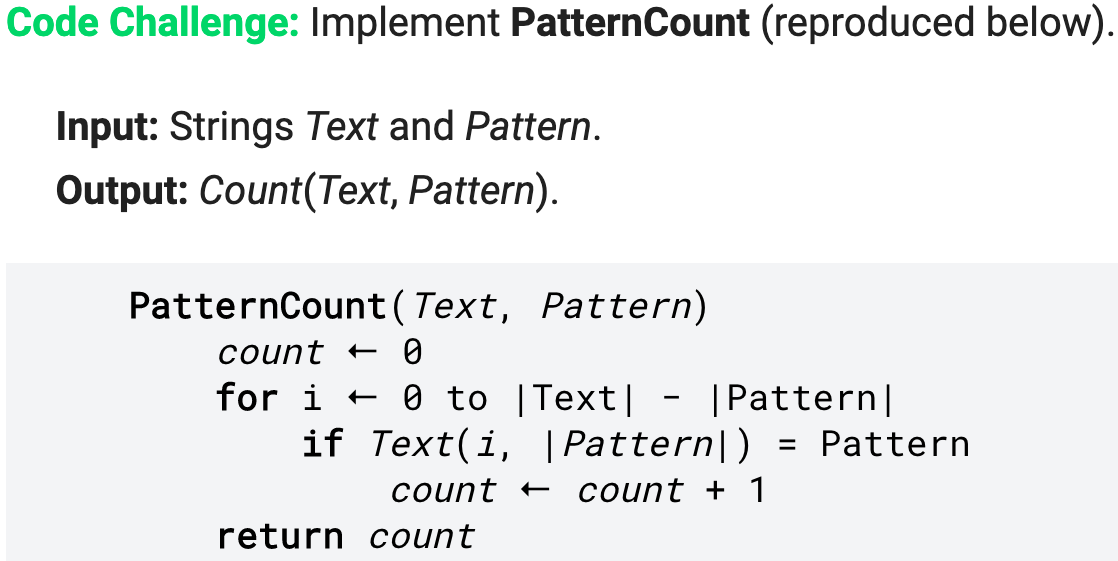
\includegraphics[width=0.85\textwidth]{figs/education-code-challenge-prompt}\\
(a)\\
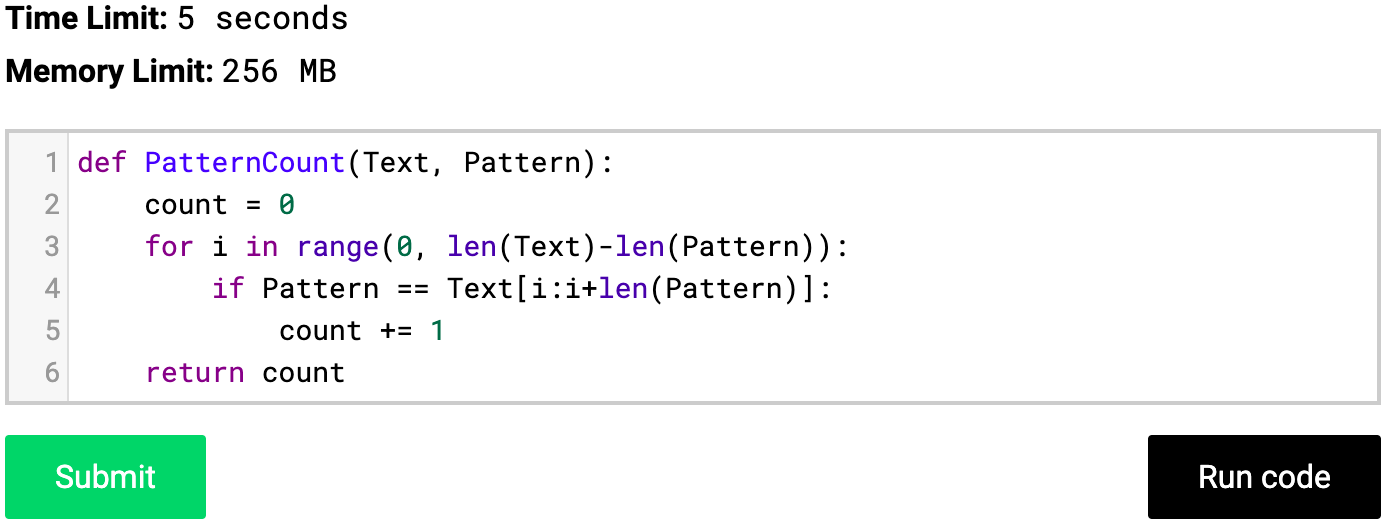
\includegraphics[width=0.85\textwidth]{figs/education-code-challenge-bug}\\
(b)\\~\\
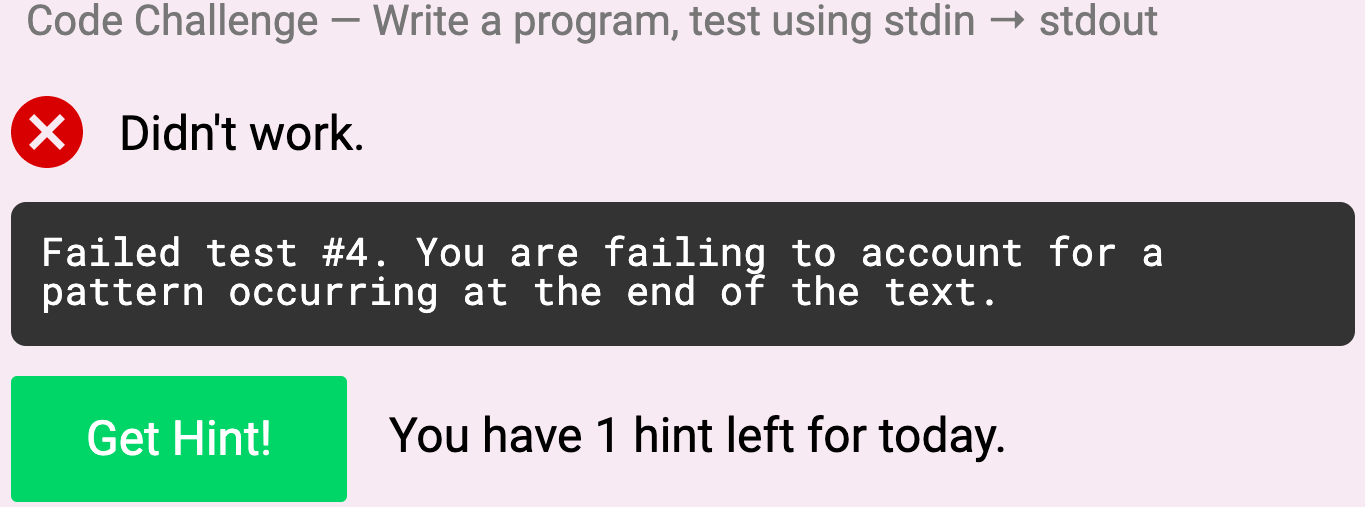
\includegraphics[width=0.85\textwidth]{figs/education-code-challenge-feedback}\\
(c)\\
\caption[Example Code Challenge]
{Example code challenge. (a) Each problem has a clear prompt, and (b) students can solve the problems directly within the text. In this example solution, the student has an off-by-one bug (the student misses the last index), and (c) the carefully-designed \gls{ITS} is able to provide the student personalized feedback.}
\label{fig:education-code-challenge}
\end{figure}

\subsubsection{Inquiry-Based Learning}
In introductory computational courses, the topics that are covered are rarely very interesting when presented out-of-context. When I present new topics in my \glspl{MAIT}, I first motivate them using a real-world problem in the form of a story. By employing Inquiry-Based Learning, an educational strategy in which students perform tasks in a fashion similar to those undertaken by professional scientists in order to construct knowledge~\cite{Pedaste2015}.

\subsubsection{Discovery Learning}
Research into Discovery Learning has showed that, when a student finds the solution to an open-ended problem on their own, the student benefits two-fold: the student typically has a stronger fundamental understanding of the solution, and the student has an improved perception of his or her own abilities to solve problems of this nature~\cite{Bruner1961}. In my \glspl{MAIT}, instead of simply presenting the learning goal to the student, I try to \textit{guide} the students and have them discover the solution on their own.

\subsubsection{Making Learning Fun!}
In my own experiences as a student, I often found it difficult to complete assigned reading assignments and would quickly lose interest during classes. In computational textbooks and learning resources, I often felt as though the learning materials were presented in a manner that was unneededly dry and complex. Instead, I fill my \glspl{MAIT} with stories, jokes, and puns, and I attempt to avoid the use of unnecessarily complex jargon when describing concepts to ensure that students of a wide range of backgrounds are able to follow successfully. I believe the success to learning is in the hands of the \textit{learners}, and it is the responsibility of the teacher as the expert to design the educational journey to be genuinely captivating. Intuitively, it is much easier to teach when students \textit{want} to learn.

\section{Results}
I developed \textit{Analyze Your Genome!} (2017), a \gls{MOOC} designed to teach biologists the best-practice workflows to analyze biological big data~\cite{Moshiri2017b}. However, instead of discussing the specifics of the algorithms behind the analyses, I focused on how to design, execute, and interpret end-to-end bioinformatics experiments. With this approach, students are able to gain the basic proficiency required to perform relevant analyses to complement their traditional biological experiments. The course covered differential gene expression analysis using \gls{RNA}-sequencing data, variant calling using \gls{WGS} vs. \gls{WES} data, rare variant calling and phasing using \gls{WGS} data obtained from a trio (i.e., mother, father, and child), and bacterial genome assembly.

I also developed \textit{Data Structures}, a \gls{MAIT} to accompany the \textit{Advanced Data Structures} course at the University of California, San Diego. Since its initial development, it has been integrated into data structures courses at the University of San Diego and the University of Puerto Rico. In 2017, the \gls{MAIT} was integrated into a \gls{MOOC} on edX: \textit{Data Structures: An Active Learning Approach} (2017)~\cite{Moshiri2017a}. The goal of the \gls{MOOC} was to bridge the gap between introductory programming (which exists in many \glspl{MOOC}) and the \textit{Bioinformatics Algorithms} \glspl{MOOC} by Compeau and Pevzner. After the large success of the \gls{MOOC}, the \gls{MAIT} was adapted to a physical textbook: \textit{Design and Analysis of Data Structures} (2018)~\cite{Moshiri2018c}. In total, \textit{Data Structures} has reached a total of nearly 40,000 learners in less than 3 years of existence, and the learners span a wide range of ages, education levels, and countries (Fig.~\ref{fig:education-learner-demographics}).

\begin{figure}
\centering
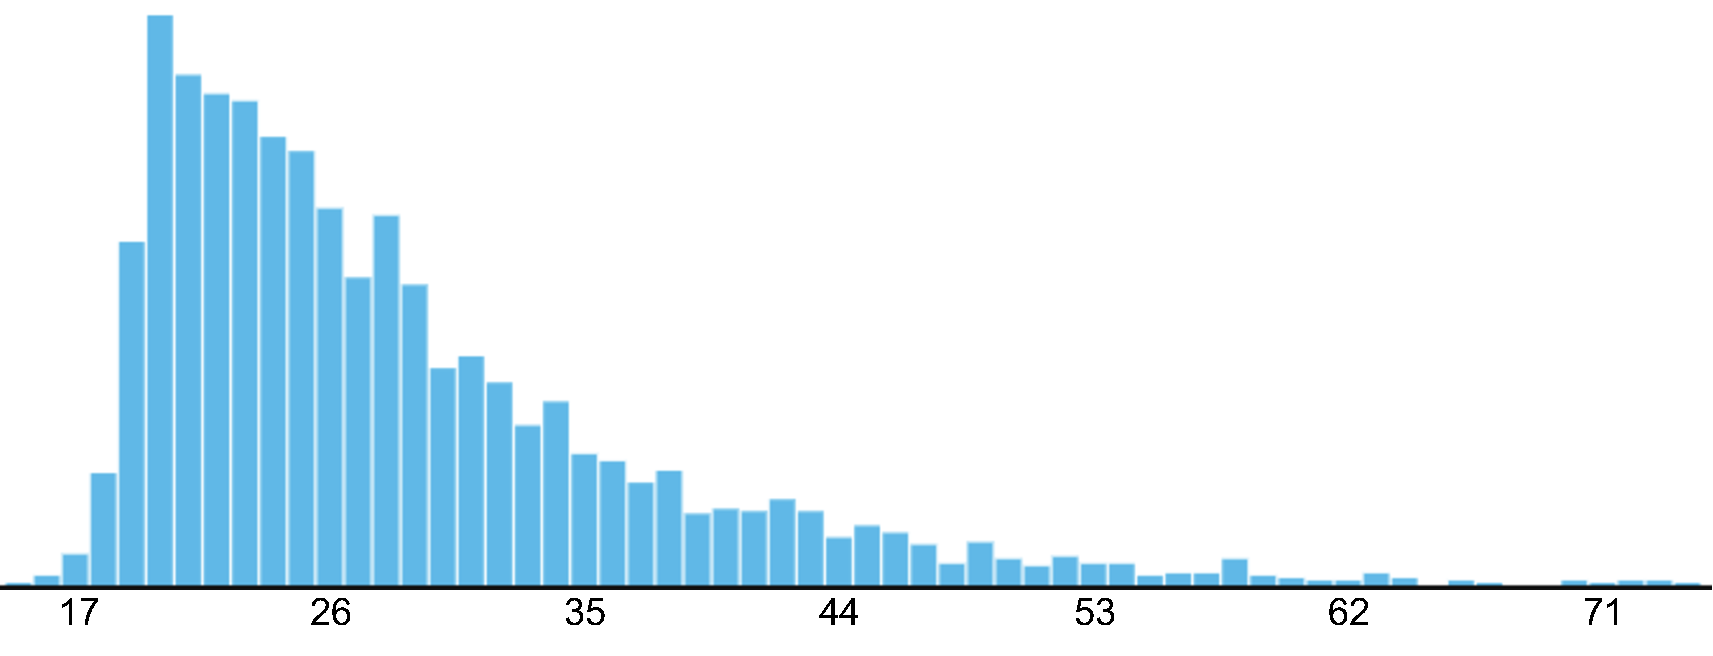
\includegraphics[width=0.85\textwidth]{figs/education-data-structures-learner-ages}\\
(a)\\
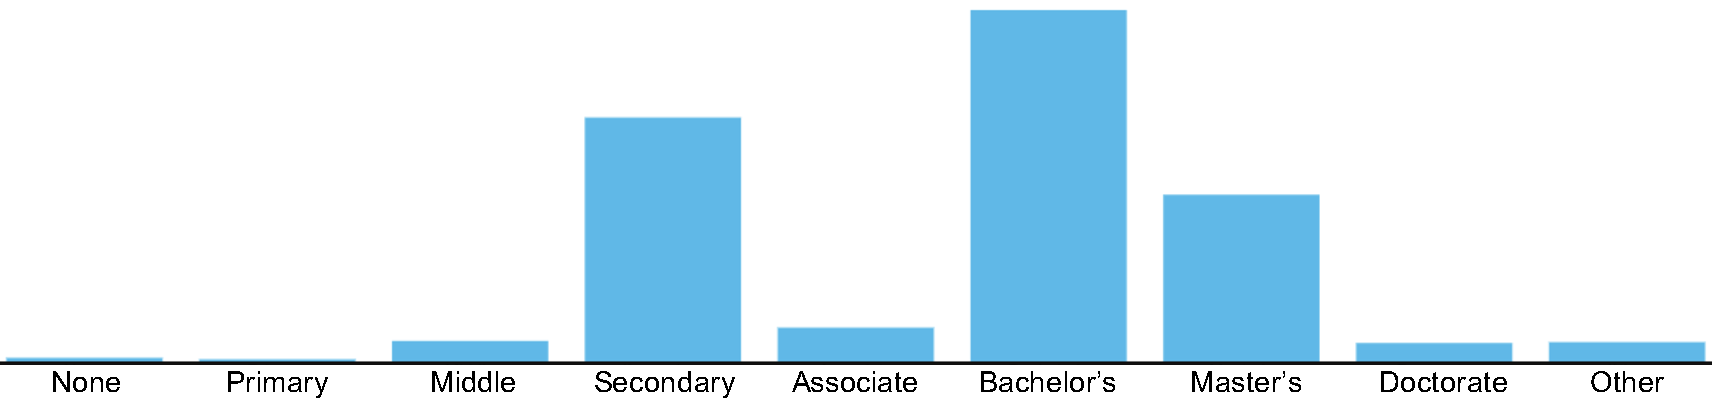
\includegraphics[width=0.85\textwidth]{figs/education-data-structures-learner-education-levels}\\
(b)\\~\\
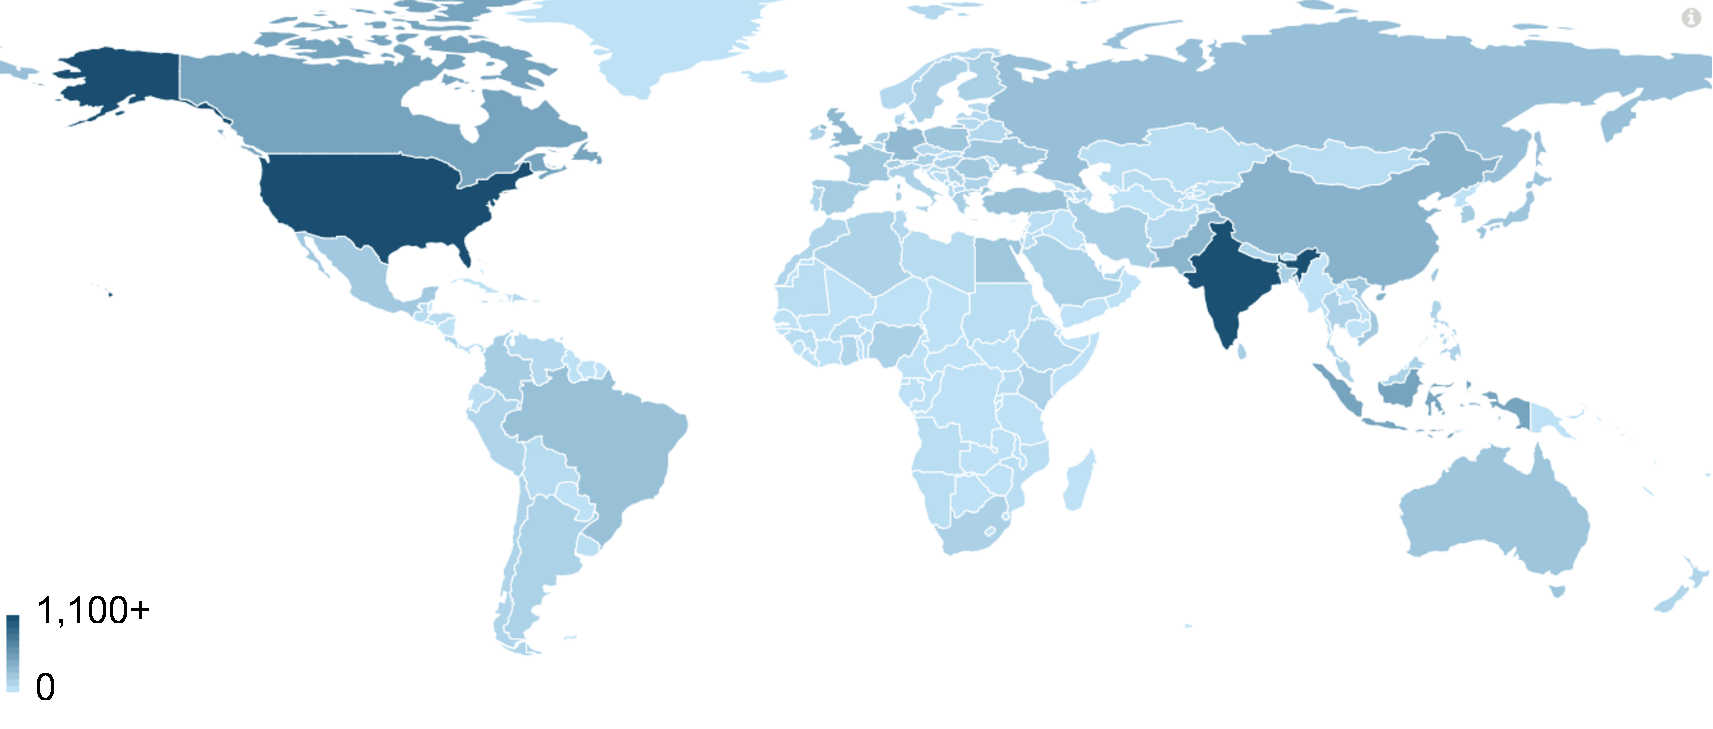
\includegraphics[width=0.85\textwidth]{figs/education-data-structures-learner-country}\\
(c)\\
\caption[Learner Demographics]
{(a) Age distribution, (b) education level distribution, and (c) geographical locations of learners in \textit{Data Structures: An Active Learning Approach}.}
\label{fig:education-learner-demographics}
\end{figure}

\section{Discussion}
Historically, the ability to learn computer science and bioinformatics has been restricted to students in higher education institutions, which can be prohibitive due to financial hardship, time constraints, or other factors. However, due to their self-paced nature, \glspl{MOOC} reduce these barriers to entry, permitting entrance by previously underrepresented demographics. For example, data structures are typically only taught in undergraduate computer science courses, meaning the distribution of students is predominantly within the range of 17 through early 20s, whereas my \gls{MOOC} has reached a far wider range of learners who would otherwise not take such a course (Fig.~\ref{fig:education-learner-demographics}a). Further, MOOCs serve as a unique opportunity for learners who may have formal education in one field but wish to transition fields, such as biologists with Bachelors, Masters, or even Doctorate levels of education who wish to learn introductory computer science (Fig.~\ref{fig:education-learner-demographics}b). Lastly, \glspl{MOOC} are accessible to curious minds across the globe, thus enabling the education of individuals who physically would not be able to attend a top university (Fig.~\ref{fig:education-learner-demographics}c).

Of course, the success of my \gls{MAIT}-based \glspl{MOOC} is largely due to the topics I have chosen, which happen to align well with the automation capabilities of online learning platforms. Specifically, the challenges in my \glspl{MOOC} are largely coding-focused, and it is typically simple to objectively determine the correctness of a student's code. However, topics in other fields (such as the social sciences) may not experience this simple objectivity in assessing correctness, which could lead to difficulties in developing \glspl{ITS} to automate grading and provide personalized feedback. Even within Computer Science and Bioinformatics, coding-focused courses may be prime for this form of presentation, but more theoretical or proof-based courses will certainly not enjoy the same ease of design.

Further, not all students in the same way, and just like any other educational technology or mode of instruction, \glspl{MAIT} may not be the optimal mode of instruction for all students. For example, some students strongly prefer the ability to directly interact with their instructor, and while online education does permit real-time interaction in the form of video meetings, the student may not perceive the interaction to be as meaningful if done remotely. On the other hand, other students who feel lost in large lectures may actually prefer the self-paced and adaptive nature of \glspl{MAIT}, which can provide them a far more personalized learning experience than can an instructor teaching 300+ other students simultaneously.

In short, I believe that, when designed carefully and executed properly, a \gls{MAIT} can be a powerful tool for improving learning and for allowing instructors to reach a massive number of individuals in a highly-scalable fashion. In the future, I will continue to develop high-quality \glspl{MAIT} to address the learning needs of the bioinformatics community.

%% END EDUCATION CHAPTER

%% Appendix
\appendix
%% START FAVITES SUPPLEMENT
\chapter{Supplemental Material for Chapter~\ref{chap:favites}}
\label{chap:favites-sup}
\clearpage

\begin{table}[!ht]
\caption[Comparison with Existing Simulation Tools]{Comparison with Existing Simulation Tools}
\vspace{-0.25in}
\begin{center}
\begin{tabular}{|P{0.8in}|P{0.5in}|P{0.8in}|P{0.8in}|P{0.6in}|P{0.8in}|P{0.8in}|}
\hline
 & \textbf{epinet} & \textbf{TreeSim} & \textbf{outbreaker} & \textbf{seedy} & \textbf{PANGEA} & \textbf{FAVITES} \\
\hline
\textbf{Contact Network} & Fixed & Complete & Complete & Complete & Fixed & Any \\
\hline
\textbf{Trans. Network} & Fixed & Fixed & Fixed & Fixed & Fixed & Any\\
\hline
\textbf{Sampling} & N/A & Fixed or \newline Sequential & Fixed & Uniform & Fixed & Any \\
\hline
\textbf{Phylogeny} & None & Fixed & Fixed & Fixed & Coalescent & Any \\
\hline
\textbf{Mutation Rate} & N/A & N/A & Constant & Constant & Fixed & Any \\
\hline
\textbf{Sequences} & None & None & Fixed & Fixed & Fixed & Any \\
\hline
\textbf{Sequencing} & N/A & N/A & No & No & No & Any \\
\hline
\end{tabular}
\end{center}
\label{tab:favites-comparison}
\end{table}

\begin{table}[!ht]
\caption[Post-Validation Tools]{Post-Validation Tools}
\vspace{-0.25in}
\begin{center}
\begin{tabular}{|P{2.3in}|P{3.7in}|}
\hline
\textbf{Name} & \textbf{Description}  \\
\hline
compare\_contact\_networks.py & Compare the degree distributions of a given simulated contact network against a reference contact network \\
\hline
compare\_trees.py & Compare the distributions of all branch lengths, internal branch lengths, terminal branch lengths, and root-to-tip distances between a given simulated tree against a given reference tree \\
\hline
distribution\_distance.py & Compute a distance between two distributions given samples from each \\
\hline
ltt.py & Create a \gls{LTT} plot from one or more Newick trees \\
\hline
sequence\_score\_profile\_HMM.py & Score a given sequence dataset against a given profile \gls{HMM} \\
\hline
\end{tabular}
\end{center}
\label{tab:favites-post-validation}
\end{table}

\begin{table}[!ht]
\caption[Helper Scripts]{Helper Scripts}
\vspace{-0.25in}
\begin{center}
\begin{tabular}{|P{2.75in}|P{3.25in}|}
\hline
\textbf{Name} & \textbf{Description}  \\
\hline
clean\_labels.py & For each read of the given sequence file or each leaf of a given phylogenetic tree, remove everything from the label except for the contact network individual's name \\
\hline
cluster\_previous\_time.py & Given a clustering from the simulation end time, a FAVITES-format transmission network, and a time, remove individuals who were not infected at the given time and output the resulting clusters \\
\hline
cn\_adjacency\_matrix\_to\_favites.py & Convert a given contact network from a binary adjacency matrix to the FAVITES format \\
\hline
degree\_stats.py & Given a contact or transmission network, compute various statistics of the node degree distribution \\
\hline
FAVITES2GEXF.py & Convert a FAVITES contact network and transmission network to the GEXF format \\
\hline
PANGEA\_transmissions\_to\_FAVITES.py & Convert a PANGEA transmission network into the FAVITES edge-list format \\
\hline
patristic\_distances.py & Given a phylogenetic tree, compute the pairwise distances between leaves and output the resulting distance matrix as a CSV file \\
\hline
scale\_tree.py & Given a phylogenetic tree (in the Newick format), scale all branches \\
\hline
score\_clusters.py & Score a given query clustering against a given true reference clustering \\
\hline
tn93\_to\_clusters.py & Convert tn93 output to the Cluster Picker clustering format \\
\hline
\end{tabular}
\end{center}
\label{tab:favites-helper}
\end{table}

\begin{table}[!ht]
\caption[HIV Simulation Parameters (epidemiological model)]{HIV Simulation Parameters (epidemiological model)}
\vspace{-0.25in}
\begin{center}
\begin{tabular}{|P{2in}|P{1.9in}|P{1.9in}|}
\hline
 & \textbf{San Diego} & \textbf{Uganda} \\
\hline
\textbf{CN Model} & \gls{BA} & \gls{BA} \\
\hline
\textbf{Expected Degree} & 4 & 4 \\
\hline
\textbf{Number of Seeds} & 1,500 & 15,000 \\
\hline
\textbf{$\lambda_{AU\rightarrow CU}$} (year$^{-1}$) & 8.667 & 8.667 \\
\hline
\textbf{$\lambda_{AT\rightarrow CT}$} (year$^{-1}$) & 4.333 & 4.333 \\
\hline
\textbf{$\lambda_{U\rightarrow T}$} (year$^{-1}$) & 1 & 1 \\
\hline
\textbf{$\lambda_{T\rightarrow U}$} (year$^{-1}$) & 1 & 0.48 \\
\hline
\textbf{$\lambda_{S,AU}$} (year$^{-1}$) & 0.1125 & 0.1125 \\
\hline
\textbf{$\lambda_{S,AC}$} (year$^{-1}$) & 0.0225 & 0.0225 \\
\hline
\textbf{$\lambda_{S,AT}$} (year$^{-1}$) & 0.005625 & 0.005625 \\
\hline
\textbf{$\lambda_{S,CT}$} (year$^{-1}$) & 0 & 0 \\
\hline
%\textbf{Rate from Acute Treated to Chronic Treated} & 
\end{tabular}
\end{center}
\label{tab:favites-params-epi}
\end{table}

\begin{table}[!ht]
\caption[HIV Simulation Parameters (evolutionary model)]{HIV Simulation Parameters (evolutionary model)}
\vspace{-0.25in}
\begin{center}
\begin{tabular}{|P{2in}|P{1.9in}|P{1.9in}|}
\hline
 & \textbf{San Diego} & \textbf{Uganda} \\
\hline
\textbf{Seed Height} (years) & 25 & 25 \\
\hline
\textbf{Seed Rate} & $1 + e^{-t^2}$ & $1 + e^{-t^2}$ \\
\hline
\textbf{Population Growth} & 2.852 & 2.852 \\
\hline
\textbf{v.T50} & -2 & -2 \\
\hline
\textbf{Mutation Rate Location} & 0.0008 & 0.001 \\
\hline
\textbf{Mutation Rate Scale} & 0.0005 & 0.0005 \\
\hline
\textbf{\gls{GTR} $\pi_A$} & 0.392 & 0.377 \\
\hline
\textbf{\gls{GTR} $\pi_C$} & 0.164 & 0.172 \\
\hline
\textbf{\gls{GTR} $\pi_G$} & 0.212 & 0.210 \\
\hline
\textbf{\gls{GTR} $\pi_T$} & 0.232 & 0.241 \\
\hline
\textbf{\gls{GTR} $\pi_{AC}$} & 1.812 & 1.388 \\
\hline
\textbf{\gls{GTR} $\pi_{AG}$} & 9.934 & 7.017 \\
\hline
\textbf{\gls{GTR} $\pi_{AT}$} & 0.718 & 0.736 \\
\hline
\textbf{\gls{GTR} $\pi_{CG}$} & 0.971 & 0.594 \\
\hline
\textbf{\gls{GTR} $\pi_{CT}$} & 9.934 & 8.618 \\
\hline
\textbf{\gls{GTR} $\pi_{GT}$} & 1 & 1 \\
\hline
\textbf{$\alpha$} ($\Gamma$ shape) & 0.405 & 0.449 \\
\hline
\end{tabular}
\end{center}
\label{tab:favites-params-evo}
\end{table}

\begin{figure}[h] 
\centering
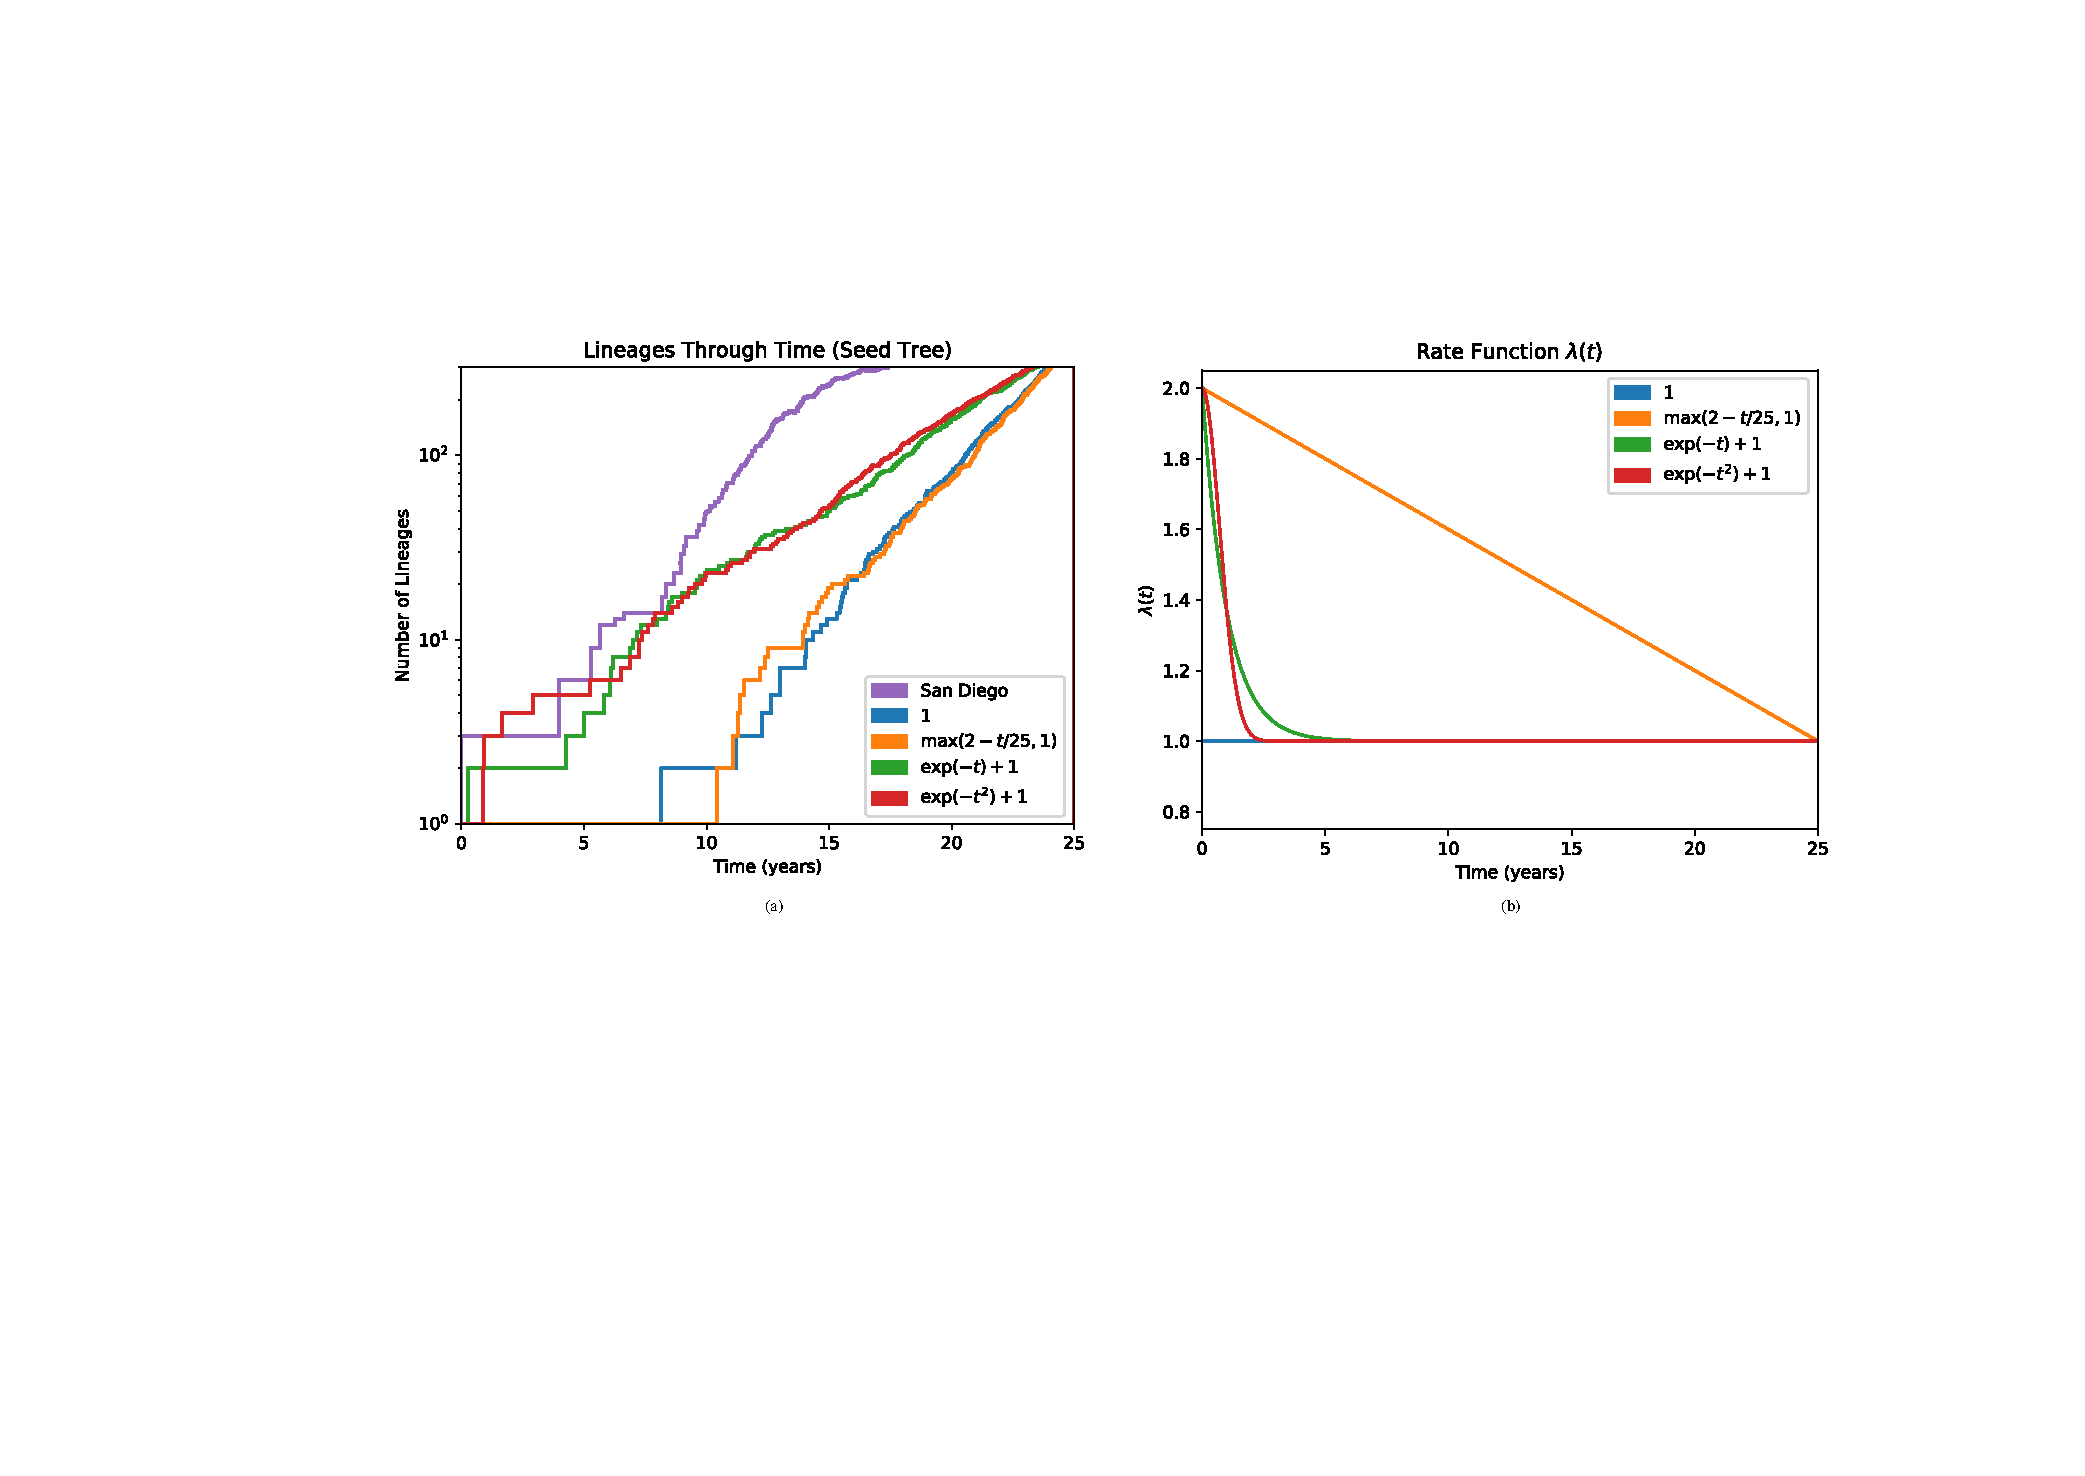
\includegraphics[width=\textwidth]{figs/favites-seed-tree}
\caption[Seed Tree]
{(a) \gls{LTT} plot of the first 25 years of the dated San Diego tree along with multiple potential rate functions for the non-homogeneous Yule model~\cite{LeGat2016}, and (b) plots of the rate functions. Because HIV trees have more short branches than normal Yule models (i.e., rate 1), we looked for functions that lead to increased numbers of lineages close to the root. This can be done by increasing the rate close to the root and then gradually decreasing the rate. As can be seen, $\lambda(t)=1$ and $\lambda(t)=\max(2-t/25,1)$ are far lower than the real San Diego curve. $\lambda(t)=\exp(-t)+1$ is much closer to the real curve, and $\lambda(t)=\exp(-t^2)+1$ is marginally closer than it. We chose to use $\lambda(t)=\exp(-t^2)+1$ as a result.}
\label{fig:favites-seed-tree}
\end{figure}

%% END FAVITES SUPPLEMENT
%% START DUAL-BIRTH SUPPLEMENT
\chapter{Supplemental Material for Chapter~\ref{chap:dualbirth}}
\label{chap:dualbirth-sup}
\clearpage

\section{Theoretical Results}
\label{sup:theory}\label{sup:sec:app-theory}

\subsection{Proofs}
\label{sec:dualbirth-proofs}

\begin{theorem}\label{sup:thm:TRO}
Let $X$ be a random variable (r.v.) over ordered ranked tree shapes and distributed according to the dual-birth model with parameter $r=\la/\lb$. Then, 
\begin{equation} % EQUATION S1 IN ORIGINAL PAPER
\Pr(X=\TRO;n) = \frac{r^{\RBh-1}}{\prod_{i=1}^{n-2} \big((r-1)\LB{i}+i+1\big)}
\end{equation}
where $\RBh$ is the number of right leaves in $\TRO$ and $\LB{i}$ is the number of its left branches before node $i$.
\end{theorem}
\begin{proof}{Proof (sketch)}
Consider the intervals between consecutive birth events in $\TRO$, and denote each interval by the rank of its end node (e.g. Figure~\ref{fig:dualbirth-model}a). Because $\TRO$ is ordered, branches in the interval $i$ can be ordered from left to right (including the order of parents) and assigned an index between 1 and $i+1$. Two ordered ranked tree shapes are equal iff the index of the branch where node $i$ is born is identical in the two trees for all $i\in\NV$. Seeing that two identical ordered ranked shapes have this property is trivial. The opposite direction becomes clear if the nodes that give birth at point $i$ in the two trees are mapped together; the shapes become obviously equivalent (edges are the same), but also the ranking becomes the same. Finally, the ordering is the same because of identical left to right ordering. Let $\xi_i$ denote the event that the index of the branch on which node $i$ is born in $X$ is equal to the index of $i$ in $\TRO$. Then, $\Pr(X=\TRO)=\Pr(\cap_1^{n-2} \xi_i)$.

Birth on each branch is governed by a Poisson process with rate $\la$ and $\lb$ for left and right branches, respectively. Due to the memoryless property of the exponential distribution, the length of each branch before node $i-1$ has no bearing on subsequent birth events.

Thus, given $\LB{i}$ (the number of left branches in the interval $i$), the probability of $\xi_i$ does not depend on $\xi_1\ldots \xi_{i-1}$. Therefore, $\Pr(\cap_1^{n-2} \xi_i)=\prod_1^{n-2} \Pr(\xi_i;\LB{i})$. Also, the probability that any one of the $i+1$ competing independent Poisson processes (present on different branches of the interval $i$) results in the first event is simply the ratio of its rate to the sum of all rates. Thus,
$$\Pr(\xi_i;\LB{i})=\frac{\la(1-\SD_i)+\lb\SD_i}{\LB{i}\la+\big(i+1-\LB{i}\big)\lb}
=\frac{r(1-\SD_i)+\SD_i}{(r-1)\LB{i}+(i+1)}.$$
Multiplying $\Pr(\xi_i;\LB{i})$s and manipulations gives results.
\end{proof}

\begin{theorem}\label{sup:thm:cherr}
For a tree shape $Z$ generated by the dual-birth model with $r=\la/\lb$, let $C=\CH{Z}/n$ be an r.v.; then, 
\begin{align}\label{sup:eq:cherries} % EQUATION S2 IN ORIGINAL PAPER
\lim_{n\to\infty}\mathbb{E}(C) = \frac{\sqrt{r}}{1+r+\sqrt{r}}
\end{align}
\end{theorem}

\begin{corollary}\label{sup:cor:rbh}
For an r.v.\ $N_r$ capturing the number of right (i.e., active) leaves in tree shape $T$,
\begin{align}\label{sup:eq:nr} % EQUATION S3 IN ORIGINAL PAPER
\lim_{n\to\infty}\mathbb{E}(N_r) = \frac{\sqrt{r}}{1+\sqrt{r}}
\end{align}
\end{corollary}

\begin{proof}{Proof (sketch)}\
Our proof follows the approach of McKenzie and Steel~\cite{McKenzie2000}. We categorize the terminal branches (i.e., those incident on leaves) of an ordered tree shape into four types: right branch in a cherry (Right Cherry, or RC), right branch not in a cherry (Right Non-cherry, or RN), left branch in a cherry (Left Cherry, or LC), and left branch not in a cherry (Left Non-cherry, or LN). Note that the number of RC and LC branches must be equal (they could be potentially combined, but the discussions are more clear if we keep them separate). Suppose an urn includes four types of balls RC, RN, LC, and LN, respectively corresponding to these four types of branches. As the tree is evolving, each birth event adds a child to one of existing terminal branches. Moreover, the terminal branch to be used is chosen at random (but not uniformly) from the terminal branches available at that time point. After the birth, two new terminal branches are added and the original branch turns into an internal branch. Because of the memoryless property of our process, each birth event is equivalent to removing a ball from the urn and adding two balls back to the urn. To make matters slightly more complicated, a birth can also change the type of sibling branches that have not been removed (e.g. a non-cherry can be turned to a cherry). This can be modeled by removing a ball of one type and adding another ball of another type. In total, after each round, the number of added balls of each type can be potentially negative but the total number of new balls is a positive constant of 1; this kind of urn models are referred to as an \gls{EPU}.

For \glspl{EPU}, asymptotic central list theorems exist for the distribution of balls~\cite{Smythe1996}. Specifically, an \gls{EPU} with $k$ types can be described by a matrix $A_{k\times k}$, in which $A_{ij}$ gives the number of balls of type $j$ added when a ball of type $i$ was drawn. Under certain conditions~\cite{Smythe1996}, the number of balls of type $i$ out of $n$ total balls is asymptotically normally distributed with a mean of $n\lambda_1 v_i$, where $\lambda_1$ is the principal eigenvalue of $A$ and $v$ is its left eigenvector normalized to add up to one; more precisely, the number of all ball types asymptotically has a joint normal distribution. A birth in the dual-birth model can be described by
\begin{small}
$$
A'= 
\begin{matrix} 
RC: \\
RN: \\
LC: \\
LN:
\end{matrix}
\begin{bmatrix} 
0& 0&  0& 1 \\
1& -1&  1& 1 \\
0& 1&  0& 0 \\
1& 0&  1& -1 
\end{bmatrix}
$$ 
\end{small}

Let $p$ be the branch where the birth happens and let $s$ be the sister to $p$. Each birth always adds a new RC and a new LC branch, but depending on the type $p$
other changes will occur too. If $p$ is an RC branch, an RC branch ($p$) is removed, an RC and an LC are added, and $s$ changes from LC to LN. Thus, in total, we gain one LN; hence, the first row of $A'$. A similar logic gives the third row. For the second row, note that when $p$ is an RN type, we simply remove $p$, reducing the count of RN by one, and add an RC and an LC. A similar logic gives the last row. 

A further complexity is that not all branches will have an equal chance of splitting in the dual-birth model. Each left (or right) branch is selected with a probability proportional to $\la$ (or $\lb$). We account for this by replacing each left ball with $\la/\lambda=r/(r+1)$ balls and each right ball with $\lb/\lambda=1/(r+1)$ balls. Thus, we get

\begin{small}
$$
A= \frac{1}{r+1}
\begin{bmatrix} 
0& 0&  0& 1 \\
1& -1&  1& 0 \\
0& r&  0& 0 \\
r& 0&  r& -r 
\end{bmatrix}
$$ 
\end{small}

It can be checked that our \gls{EPU} satisfies the conditions of the \gls{EPU} central list theorem. The principle eigenvalue of $A$ is $\lambda_1=\frac{\sqrt{r}}{r+1}$, and \textit{a} left eigenvector is

\begin{small}
$$
v'= 
\begin{bmatrix}1+\sqrt{r}& r&  1+\sqrt{r}& \frac{1}{1+\sqrt{r}}
\end{bmatrix}$$
\end{small} 

The results immediately follow by computing $\lambda_1v'_1/\sum_1^4 v'_i$ for $\mathbb{E}(C)$ and $\lambda_1(v'_1+v'_2)/\sum_1^4 v'_i$ for $\mathbb{E}(N_r)$.
\end{proof}

\begin{theorem}
For a weighted tree shape $t$ generated by the dual-birth model with parameters $r$ and $\lambda$ conditioned on having $n$ leaves, let $\BL$ be an r.v.\ giving the length of a random branch in $t$; i.e., $\BL=\bl_I$ for $I\sim\mathcal{U}(1,n-2$). Then, 
\begin{align}\label{sup:eq:bl} % EQUATION S4 IN ORIGINAL PAPER
\lim_{n\to\infty}\mathbb{E}(\BL) \to \frac{1}{2\lambda}\left(\frac{r+1}{\sqrt{r}}\right)
\end{align}
\end{theorem}

\begin{proof}{Proof (sketch)}
It is constructive to think about the sampling strategy. First, an \textit{uncensored} tree is created with $n$ terminal branches but with varying depth for leaves. Half of the branches in this tree are drawn from the exponential distribution with rate $\la$ and the other half with rate $\lb$. Thus, the expected sum of branch lengths in the uncensored tree is $\frac{1}{2}(\frac{1}{\la}+\frac{1}{\lb})n$. We then cut $n-1$ branches. Because of the memoryless property of the exponential distribution, the expected length of the branches we cut from a tip is $1/\lb$ for right branches and $1/\la$ for left branches. By the proof of Corollary~\ref{cor:rbh}, the number of left and right branches are normally distributed with known expectation (Eq.~\ref{eq:bl}); thus,
$$
\mathbb{E}(\BL)=
\frac{1}{n}\left(\frac{n}{2\la}+\frac{n}{2\lb}-\left(\frac{\sqrt{r}}{1+\sqrt{r}}\frac{1}{\lb}+\frac{1}{1+\sqrt{r}}\frac{1}{\la}\right)(n-1)\right)
$$
which in limit gives the results. 
\end{proof}

\begin{lemma}\label{lem:cherryparsimony} % LEMMA S1 IN ORIGINAL PAPER
For a tree shape $t$, the most parsimonious number of activation events is the minimum number of activation events possible, which is equal to the number of cherries in $t$.
\end{lemma}

\begin{proof}{Proof}
First, the most parsimonious number of activation events is the minimum number of activation events possible. As mentioned in the main paper, an activation event is a biological change, so a most parsimonious number of activation events would be one that minimizes the number of activation events. Note that, under the dual-birth model, the root node is considered an activation event.

Next, we prove that the minimum number of activation events possible is equal to the number of cherries in $t$. Let $N_t$ represent the minimum number of activation events possible for tree $t$, let $V_t$ denote the set of nodes in $t$, and let $a_v = 1$ if an activation event occurs on node $v$, otherwise $a_v = 0$. Under the dual-birth model, activation events only occur on nodes (i.e., not on edges), so $N_t = \sum_{v \in V}{a_v}$.

A node $v$ can have either 0 or 2 children. Under the dual-birth model, activation events occur when an inactive node gives birth to a new node, meaning activation events can only occur on internal nodes of $t$. Leaves that are active cannot undergo an activation event (by definition), and leaves that are inactive have not yet given birth, meaning they have not yet been activated. Therefore, for all leaves $f$, $a_f = 0$.

For an internal node $v$, there are three possible cases: both children of $v$ are leaves (i.e., $v$ is a cherry), one child is a leaf and the other is an internal node, or both children of $v$ are internal nodes.

If both children of $v$ are leaves (i.e., $v$ is a cherry), by definition, one child is active (and is therefore the propagation of $v$), and the other child is inactive. Therefore, either $v$ or an ancestor of $v$ must have undergone an activation event. Let $A_v$ denote the set of ancestors of node $v$. Because the dual-birth model does not allow deactivation, there can only be a single activation event in the lineage of an active node, meaning $a_v + \sum_{u \in A_v}{a_u} = 1$.

If one child of $v$ is an internal node and the other is a leaf, let $c$ denote the child that is an internal node. One of the descendants of $c$ must be a cherry. Therefore, there must be a cherry $u$ such that $v \in A_u$.

If both children of $v$ are internal nodes, by the same logic of the previous paragraph, $v$ must be the ancestor of at least two cherries: one for each of its internal node children.

Therefore, because each lineage of a cherry must have exactly 1 activation event, and because every internal node that is not a cherry much be in the lineage of a cherry, the minimum number of activation events possible would be a single activation event for each cherry's lineage. Therefore, the minimum number of activation events is equal to the number of cherries in $t$.
\end{proof}

\subsection{Set of All Possible Orderings}
For $\TR \defeq(T,\RN)$, the set $\SDALL(\TR)$ of all possible orderings for $\TR$ (as shown in Figure~\ref{fig:dualbirth-model}c of the main paper) can be constructed recursively. For an internal node $u$ and its two children $\child{u}{1}$ and $\child{u}{2}$, let
\begin{equation*}
\SDALL'(\{u\}) =
\begin{cases}
\{\{(\child{u}{1},0),(\child{u}{2},1)\},\{(\child{u}{2},0),(\child{u}{1},1)\}\}
&  \text{if } \child{u}{1},\child{u}{2}\neq \leaf \\
\{\{(\child{u}{2},0)\},\{(\child{u}{2},1)\}\} 
& \text{if } \child{u}{1}= \leaf\\
\{\{(\child{u}{1},0)\},\{(\child{u}{1},1)\} \}
& \text{if } \child{u}{2}= \leaf\\
\{\{\}\} &  \text{if } \child{u}{1}=\child{u}{2}= \leaf 
\end{cases}
\end{equation*}
\begin{small}
and for two disjoint node sets $X$ and $Y$:
\begin{equation}\label{sup:eq:sdall} % EQUATION S5 IN ORIGINAL PAPER
\SDALL'(X\cup Y) = \{\SD_X \cup \SD_Y| (\SD_X,\SD_Y ) \in \SDALL'(X) \times \SDALL'(Y)\}.
\end{equation}
\end{small}
Then, $\SDALL(\TR)=\{\SD_X\cup\{(r,1)\} | \SD_X\in \SDALL'(V)\}$ where $r$ is the root.

\section{Supplementary Methods}
\subsection{Simulation Setup}\label{sup:simsetup}
\subsubsection{Motivation of Default Parameters}\label{sup:simsetup-mot}
The default value of $n = 1,000$ (which is used for all trees in all experiments) is chosen because it is large enough to observe changes in tree shape resulting from tweaking the other parameters, yet it is small enough that simulations and subsequent tree inferences remain computationally tractable. The default values for the alignment simulation parameters, including \gls{GTR} parameters, are chosen based on ML estimates from of the \textit{Alu}  tree as computed by FastTree-2 (see Section~\ref{sec:dualbirth-human-alu-analyses}).

The default value of $r=10^{-2}$ is chosen because $r=1$ is equivalent to the Yule model and $r=10^{-4}$ results in an almost fully ladder-like tree, so $r=10^{-2}$ serves as an intermediate. The default value of $\lambda=169.328$ is chosen because the best estimate of the average branch length of the \textit{Alu} tree is 0.029824, which can be used with the default value of $r=10^{-2}$ to find $\lambda$ (Eq.~\ref{eq:bl}). $k=300$ is chosen to match the length of \textit{Alu}.

The default value of ultrametricity deviation gamma distribution rate $\alpha=29.518$ is chosen by first rooting the best estimate of the \textit{Alu} tree on the MRCA of 7SLRNA sequences, which we assume is the outgroup of the \textit{Alu} elements~\cite{Deininger2011}. Then, root-to-tip distances are computed and are normalized by the distribution average. A gamma distribution is then fit on the resulting distribution with the constraint that the distribution's rate and shape must be equal.

\subsubsection{Data Generation}
To generate ``true trees,'' we use our implementation of the generative process of the dual-birth model, which takes three parameters: $\la$, $\lb$, and $n$. We then deviate each tree from ultrametricity by multiplying each branch of the tree by a multiplier sampled from a gamma distribution with shape and rate both set to some parameter $\alpha$ (so as to keep the expected value of the distribution equal to 1, and as a result, keep the average branch lengths of the trees constant). We then simulate a multiple sequence alignment with no indels according to the \gls{GTR}+$\Gamma$ model using INDELible.

We have a series of ``experiments,'' where we start with a default set of parameters and then deviate one parameter at a time.

\begin{itemize}
\item \textbf{INDELible Parameters (Global)}
\begin{itemize}
\item \gls{GTR} Frequencies: 0.2922 0.2319 0.2401 0.2358
\item \gls{GTR} Rates (ac ag at cg ct gt): 0.8896 2.9860 0.8858 1.0657 3.8775 1.0000
\item $\alpha = 5.256$
\end{itemize}

\item \textbf{Default Parameters (param-00)}
\begin{itemize}
\item $n = 1000$ (Global)
\item $r = 10^{-2}$
\item $\la = 1.6765100539857060$
\item $\lb = 167.65100539857060$
\item Ultrametricity Gamma Distribution Parameter $\alpha = 29.518173529892621$
\item Sequence Length = 300
\end{itemize}

\item \textbf{Experiment 1 (Changing $r$) (Constant Average Branch Length)}
\begin{itemize}
\item param-04: $r = 10^{-4}$, $\la = 0.16765100539857060$, $\lb = 1676.5100539857060$
\item param-03: $r = 10^{-3}$, $\la = 0.53015902907666816$, $\lb = 530.15902907666816$
\item param-00: $r = 10^{-2}$, $\la = 1.6765100539857060$, $\lb = 167.65100539857060$
\item param-02: $r = 10^{-1}$, $\la = 5.3015902907666816$, $\lb = 53.015902907666816$
\item param-01: $r = 10^{0}$, $\la = 16.765100539857060$, $\lb = 16.765100539857060$
\end{itemize}

\item \textbf{Experiment 2 (Changing Model of DNA Evolution)}
\begin{itemize}
\item param-00: JC69
\item param-00: K80
\item param-00: HKY85
\item param-00: GTRCAT
\item param-00: \gls{GTR}+$\Gamma$
\end{itemize}

\item \textbf{Experiment 3 (Changing $\lambda$)}
\begin{itemize}
\item param-05: $\la = 0.33530201079714$, $\lb = 33.53020107971412$
\item param-06: $\la = 0.83825502699285$, $\lb = 83.8255026992853$
\item param-00: $\la = 1.6765100539857060$, $\lb = 167.65100539857060$
\item param-07: $\la = 3.35302010797141$, $\lb = 335.3020107971412$
\item param-08: $\la = 8.38255026992853$, $\lb = 838.255026992853$
\end{itemize}

\item \textbf{Experiment 4 (Changing Sequence Length)}
\begin{itemize}
\item param-09: Sequence Length = 50
\item param-10: Sequence Length = 100
\item param-11: Sequence Length = 200
\item param-00: Sequence Length = 300
\item param-12: Sequence Length = 600
\item param-13: Sequence Length = 1200
\item param-14: Sequence Length = 2400
\item param-15: Sequence Length = 4,800
\end{itemize}

\item \textbf{Experiment 5 (Changing Number of Leaves $n$)}
\begin{itemize}
\item param-25: $n = 25$
\item param-26: $n = 50$
\item param-27: $n = 250$
\item param-28: $n = 500$
\item param-00: $n = 1000$
\item param-29: $n = 2000$
\item param-30: $n = 4000$
\end{itemize}

\item \textbf{Experiment 6 (Changing Ultrametricity Gamma Distribution Parameter $\alpha$)}
\begin{itemize}
\item param-16: $\alpha = 2.95181735298926$
\item param-17: $\alpha = 5.90363470597852$
\item param-00: $\alpha = 29.518173529892621$
\item param-18: $\alpha = 147.590867649463$
\item param-19: $\alpha = 295.181735298926$
\item param-20: $\alpha = 9999999999999999$ (i.e., $\infty$)
\end{itemize}
\end{itemize}

\subsubsection{Methods}
For each alignment created by INDELible (one alignment per ``true tree''), we use FastTree-2 and RAxML to infer a tree using the \gls{GTR}+$\Gamma$ model. We run RAxML a second time on the trees outputted by RAxML in order to compute branch support values. We then estimate cherries using the method described in Section~\ref{sec:dualbirth-paramest}.
\begin{itemize}
\item \textbf{FastTree~2:} \texttt{fasttree -nt -gtr -gamma < SEQS}
\begin{itemize}
\item \texttt{-nt:} Alignment contains nucleotide sequences
\item \texttt{-gtr:} Use \gls{GTR} model
\item \texttt{-gamma:} Rescale tree's branch lengths to optimize Gamma20 likelihood
\item \texttt{SEQS:} INDELible multiple sequence alignment (FASTA)
\end{itemize}

\item \textbf{Initial RAxML (Tree Inference):} \texttt{raxmlHPC -s SEQS -m GTRGAMMA\\-n OUT -p \$RANDOM}
\begin{itemize}
\item \texttt{-s SEQS:} Specify the sequence alignment file to be \texttt{SEQS} (FASTA)
\item \texttt{-m GTRGAMMA:} Use the \gls{GTR}+$\Gamma$ model
\item \texttt{-n OUT:} Specify output project name to be \texttt{OUT}
\item \texttt{-p \$RANDOM:} Use a random number as the seed
\end{itemize}

\item \textbf{Final RAxML (Branch Support):} \texttt{raxmlHPC -f J -p \$RANDOM\\-m GTRGAMMA -s SEQS -t TREE -n OUT}
\begin{itemize}
\item \texttt{-f J:} Compute SH-like support values on the given tree
\item \texttt{-p \$RANDOM:} Use a random number as the seed
\item \texttt{-m GTRGAMMA:} Use the \gls{GTR}+$\Gamma$ model
\item \texttt{-s SEQS:} Specify the sequence alignment fileto be \texttt{SEQS} (FASTA)
\item \texttt{-t TREE:} Specify the input tree (from ``Initial RAxML'' step)
\item \texttt{-n OUT:} Specify output project name to be \texttt{OUT}
\end{itemize}

\item \textbf{Cherry Estimation:} \texttt{estimate-cherries.sh TREE THRESHOLD}
\begin{itemize}
\item \texttt{TREE:} Tree for which to estimate cherries
\item \texttt{THRESHOLD:} Branch support threshold to use
\end{itemize}
\end{itemize}

\subsubsection{Error Measurement}
We measure the accuracy of inferred tree topology using the \gls{RF} distance as well as the \gls{MS} metric.

\begin{itemize}
\item \textbf{RF Computation:} \texttt{echo \$(echo -n '(' \&\&\\echo -n `compareTrees.missingBranch TRUE INFERRED | cut -d' ' -f3` \&\&\\echo -n ' + ' \&\&\\echo -n `compareTrees.missingBranch INFERRED TRUE | cut -d' ' -f3` \&\&\\echo -n ') / 2') | bc -l}
\begin{itemize}
\item \texttt{TRUE:} ``True tree'' simulated by our dual-birth simulation tool
\item \texttt{INFERRED:} Inferred tree (from either FastTree~2 or RAxML)
\item \texttt{compareTrees.missingBranch:} Tool to compute missing branch rate (FN) between two trees
\item First compute FN of \texttt{INFERRED} with respect to \texttt{TRUE}
\item Then compute FN of \texttt{TRUE} with respect to \texttt{INFERRED}
\item Average these two FN values to compute the RF metric
\end{itemize}

\item \textbf{\gls{MS} Computation:} \texttt{TreeCmp.jar -r TRUE -d ms -i INFERRED}
\begin{itemize}
\item \texttt{TRUE:} ``True tree'' simulated by our dual-birth simulation tool
\item \texttt{INFERRED:} Inferred tree (from either FastTree~2 or RAxML)
\item \texttt{TreeCmp.jar:} Tool used to compute MS metric~\cite{Bogdanowicz2012}
\item \texttt{-r TRUE:} Specify \texttt{TRUE} to be the reference tree
\item \texttt{-d ms:} Compute the MS distance metric
\item \texttt{-i INFERRED:} Specify \texttt{INFERRED} to be the inferred tree
\end{itemize}
\end{itemize}

\subsection{Human \textit{Alu} Analyses}
\subsubsection{Data Acquisition}\label{sup:aludata}
\begin{itemize}
\item \textbf{DfamScan:} \texttt{dfamscan.pl -fastafile hg19.fa -hmmfile Dfam-Alu.hmm\\-dfam\_outfile hg19.out}
\begin{itemize}
\item \texttt{-fastafile hg19.fa:} Specify the hg19 reference genome as the input
\item \texttt{-hmmfile Dfam-Alu.hmm:} Use the \textit{Alu} Dfam HMM database
\item \texttt{-dfam\_outfile hg19.out:} Output results to \texttt{hg19.out}
\end{itemize}
\end{itemize}

\subsubsection{Alignment and Tree Inference}\label{sup:alualignment}
Our first dataset of the ``\textit{Alu}'' family based on the Dfam database included non-\textit{Alu} items (e.g. 7SLRNA, which is thought to be a predecessor of \textit{Alu} elements). Our initial analyses included these non-\textit{Alu} members of the Dfam \textit{Alu} family, which resulted in poor placement of these more ancestral repeats on the resulting tree. We filtered out these non-\textit{Alu} elements and recomputed both alignments and trees. Our online data include both filtered and unfiltered datasets. 

%% Figures
\section{Supplementary Figures}
\begin{figure} % FIGURE S1 IN ORIGINAL PAPER
\centering
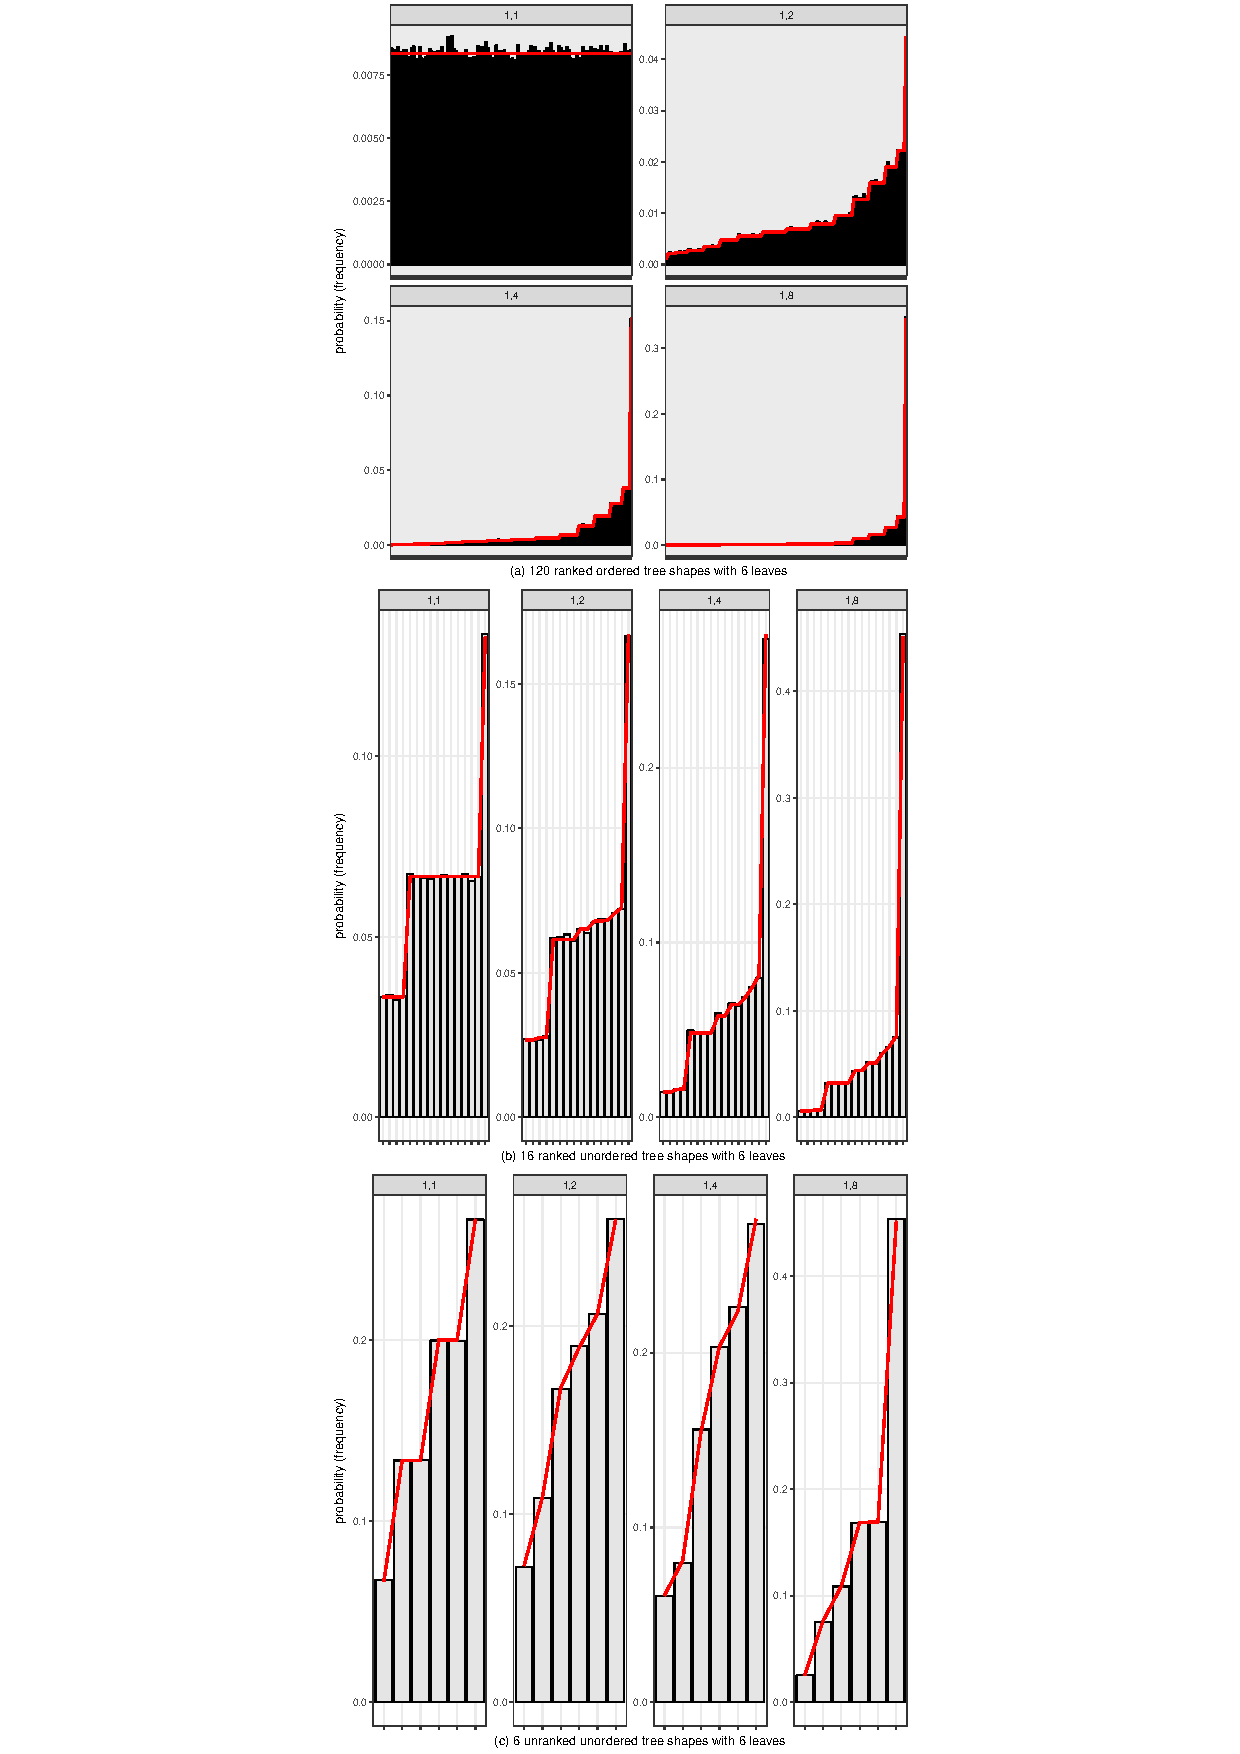
\includegraphics[width=0.35\textwidth]{figs/dualbirth-tree-prob-dists}
\caption[Probability distributions on ranked tree shapes]
{Probability distributions on ranked tree shapes. There are (a) 120 ranked ordered tree shapes, (b) 16 ranked unordered tree shapes, and (c) 6 unranked unordered tree shapes with $n=6$. The distribution according to the dual-birth model is given over these trees for four choices of $\la$ and $\lb$ (box header) corresponding to $r=1$ (i.e., Yule), $r=1/2$, $r=1/4$, and $r=1/8$. Red line gives the theoretical distribution and the grey bars give the frequencies in 100,000 simulations.}
\label{fig:dualbirth-tree-prob-dists}
\end{figure}

\begin{figure} % FIGURE S2 IN ORIGINAL PAPER
\centering
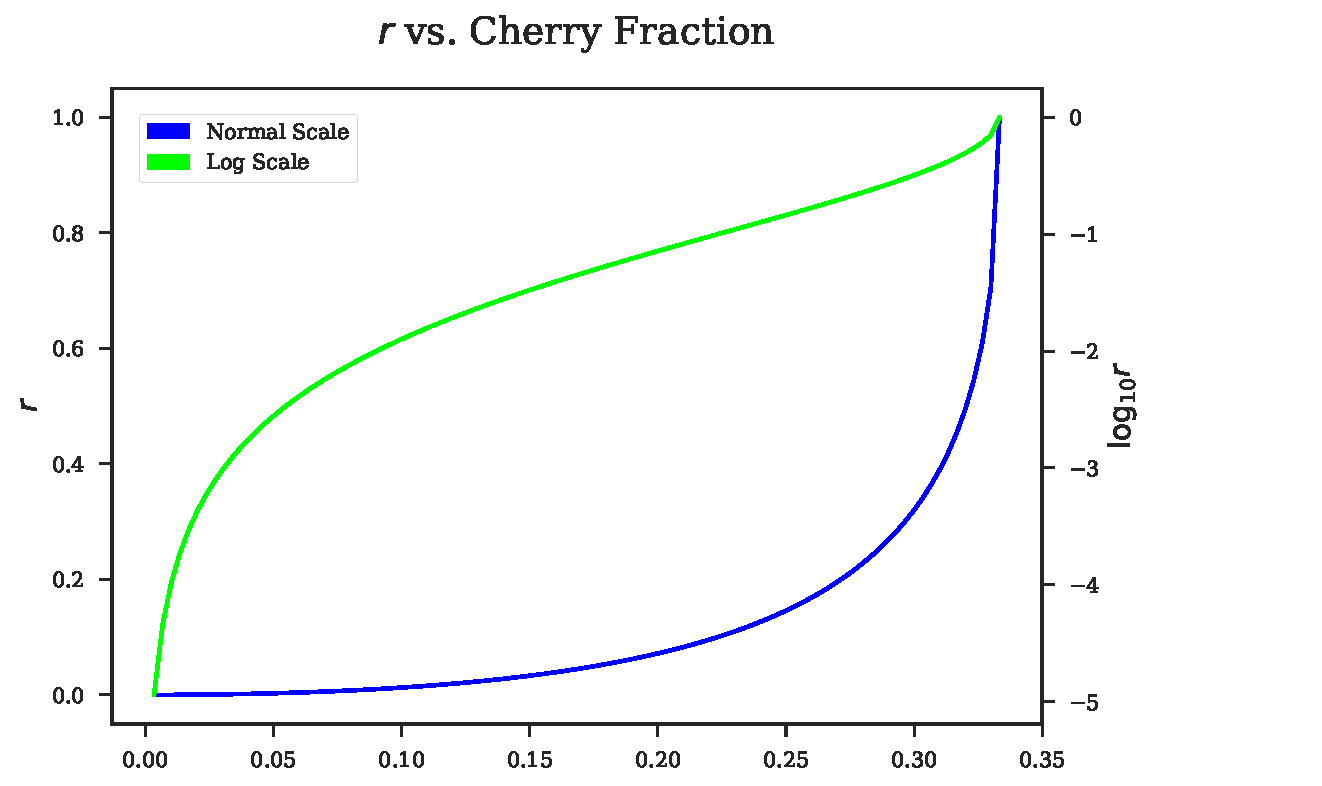
\includegraphics[width=0.8\textwidth]{figs/dualbirth-sup-cvsr}
\caption[Estimated $r$ vs. Cherry Fraction]
{Estimated $r$ vs. Cherry Fraction. Estimated $r$ ($y$-axis) as a function of the fraction of cherries ($x$-axis). Blue (left axis) shows normal scale and green (right) shows the logarithmic scale.}
\label{fig:dualbirth-sup-cvsr}
\end{figure}

\begin{figure} % FIGURE S3 IN ORIGINAL PAPER
\centering
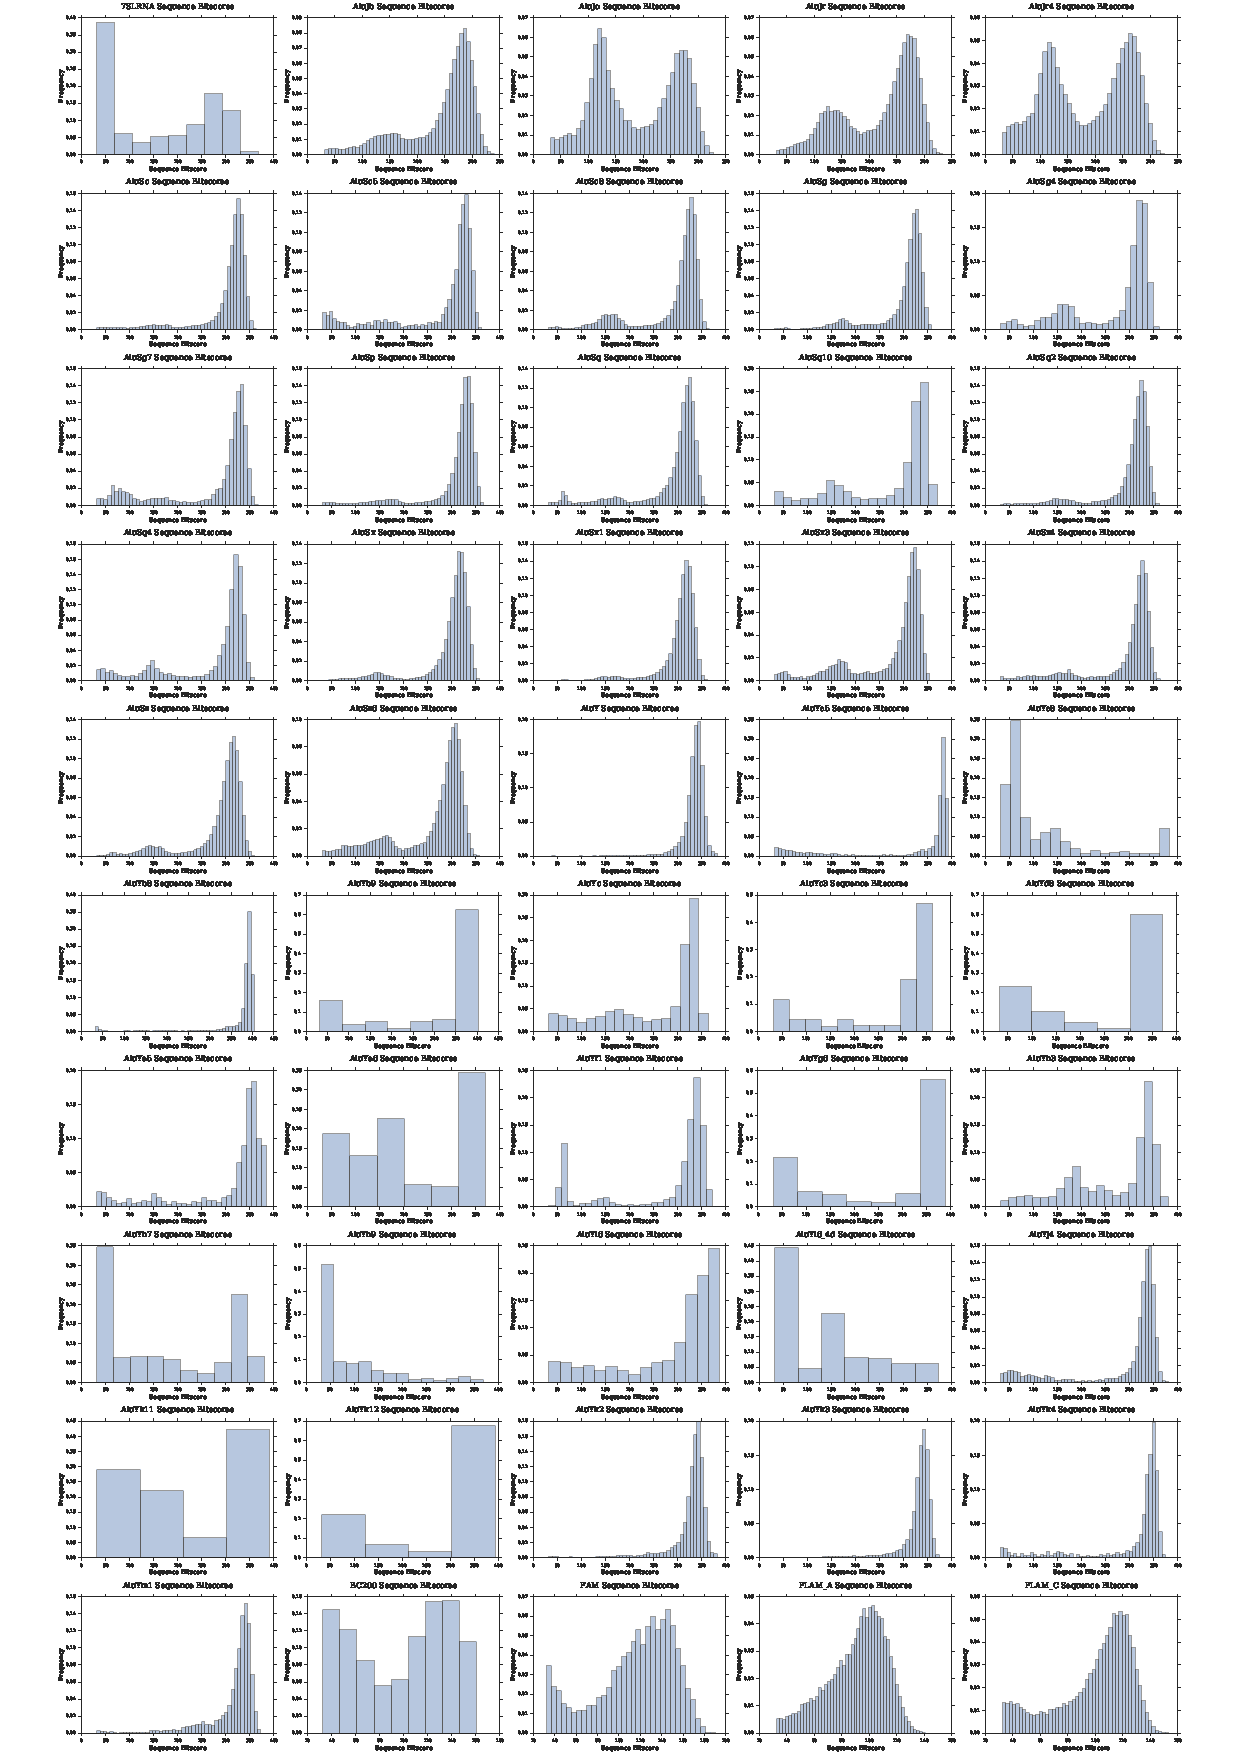
\includegraphics[width=0.8\textwidth]{figs/dualbirth-bit-hists}
\caption[Histograms of bitscores]
{Histograms of bitscores.}
\label{fig:dualbirth-bit-hists}
\end{figure}

\begin{figure} % FIGURE S4 IN ORIGINAL PAPER
\centering
\begin{small}
\begin{tabular}{c c c c c c c c}\hline
7SLRNA&AluJb&AluJo&AluJr&AluJr4&AluSc&AluSc5&AluSc8\\
200   &200  &200  &225  &200   &275  &275   &275\\\hline
AluSg&AluSg4&AluSg7&AluSp&AluSq&AluSq10&AluSq2&AluSq4\\
275  &275   &275   &275  &275  &275    &275   &250\\\hline
AluSx&AluSx1&AluSx3&AluSx4&AluSz&AluSz6&AluY&AluYa5\\
250  &250   &250   &250   &250  &250   &300 &325\\\hline
AluYa8&AluYb8&AluYb9&AluYc&AluYc3&AluYd8&AluYe5&AluYe6\\
100   &250   &250   &275  &300   &300   &300   &300\\\hline
AluYf1&AluYg6&AluYh3&AluYh7&AluYh9&AluYi6&AluYi6\_4d&AluYj4\\
300   &300   &300   &275   &200   &225   &225       &300\\\hline
AluYk11&AluYk12&AluYk2&AluYk3&AluYk4&AluYm1&BC200&FAM\\
325    &325    &250   &250   &375   &300   &100  &65\\\hline
FLAM\_A&FLAM\_C\\
80     &80\\
\hline
\end{tabular}
\end{small}
\caption[Bitscore thresholds]
{Bitscore thresholds.}
\label{fig:dualbirth-bit-thresh}
\end{figure}

\begin{figure} % FIGURE S5 IN ORIGINAL PAPER
\centering
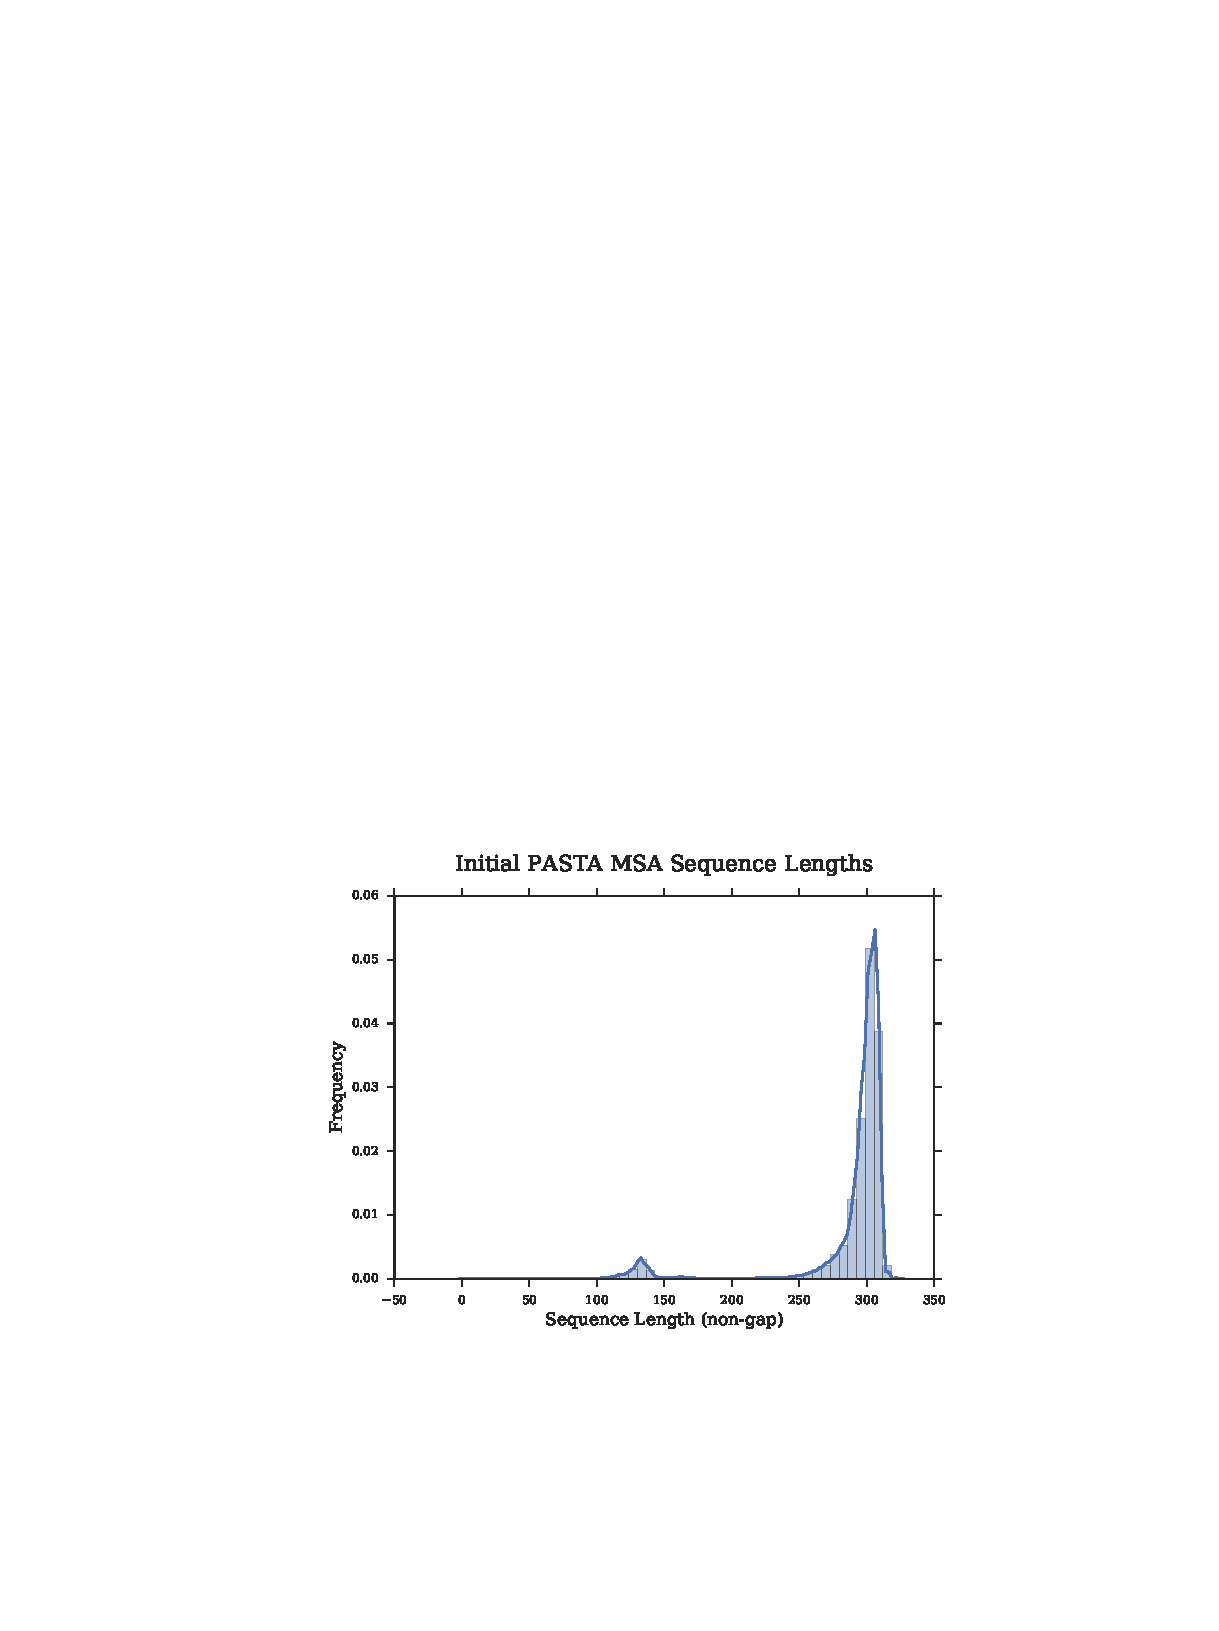
\includegraphics[width=0.9\textwidth]{figs/dualbirth-non-gap-hist}
\caption[PASTA alignment sequence lengths]
{PASTA alignment sequence lengths. Histogram of sequences based on non-gap sequence length. As can be seen, a nontrivial number of sequences in the alignment have non-gap lengths well below 300, which we know \textit{a priori} to be the typical length of \textit{ Alu} sequences.}
\label{fig:dualbirth-non-gap-hist}
\end{figure}

\begin{figure} % FIGURE S6 IN ORIGINAL PAPER
\begin{center}
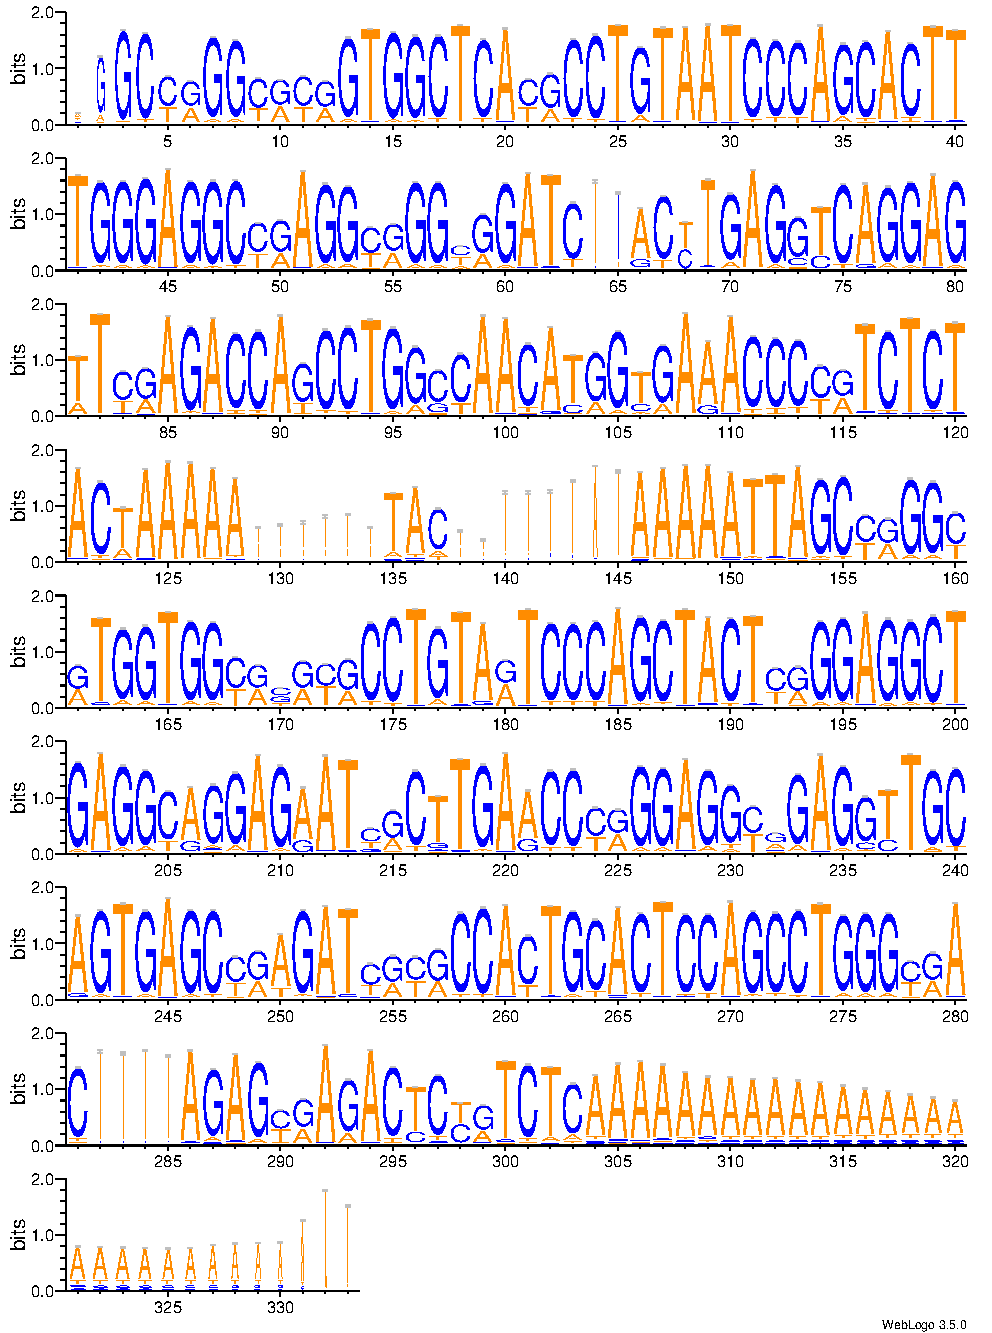
\includegraphics[width=0.45\textwidth]{figs/dualbirth-alu-tree-a.pdf}
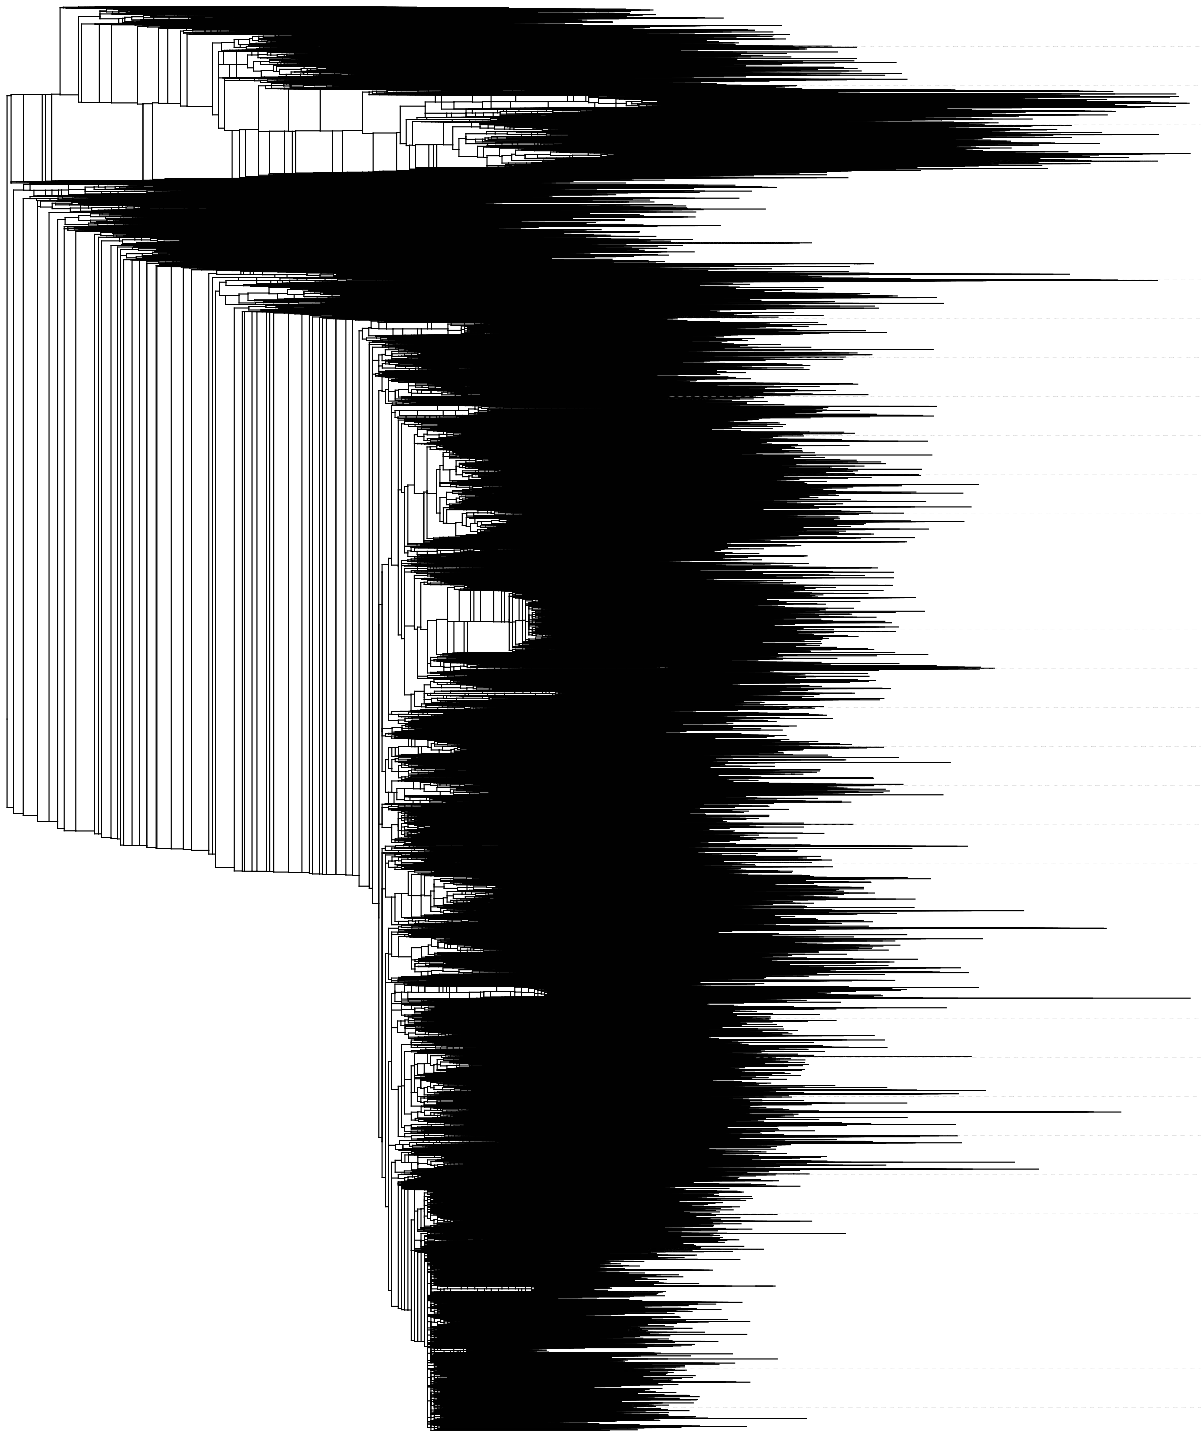
\includegraphics[width=0.45\textwidth]{figs/dualbirth-alu-tree-b.pdf}\\
(a)~~~~~~~~~~~~~~~~~~~~~~~~~~~~~~~~~~~~~~~~~~~~~~~~~~~~~~~~~~~~~~~~~(b)
\end{center}
\caption[Human \textit{Alu} alignment and tree]
{Human \textit{ Alu} alignment and tree. 
(a) Sequence logo constructed from the \textit{ Alu} multiple sequence alignment in which sequences with less than 200 non-gap characters were removed and sites with less than 1\% non-gap characters were masked, using WebLogo~\cite{Crooks2004}. The logo indicates conserved sequences and a good quality alignment: most sites have a clear high-frequency consensus nucleotide.\label{fig:dualbirth-alu-logo} (b) Midpoint-rooted \textit{ Alu} phylogenetic tree inferred from the aforementioned sequence alignment by RAxML under the \gls{GTR}+CAT model. As expected, portions of the tree are very ladder-like.}
\label{fig:dualbirth-alu-tree}
\end{figure}

\begin{figure} % FIGURE S7 IN ORIGINAL PAPER
\centering
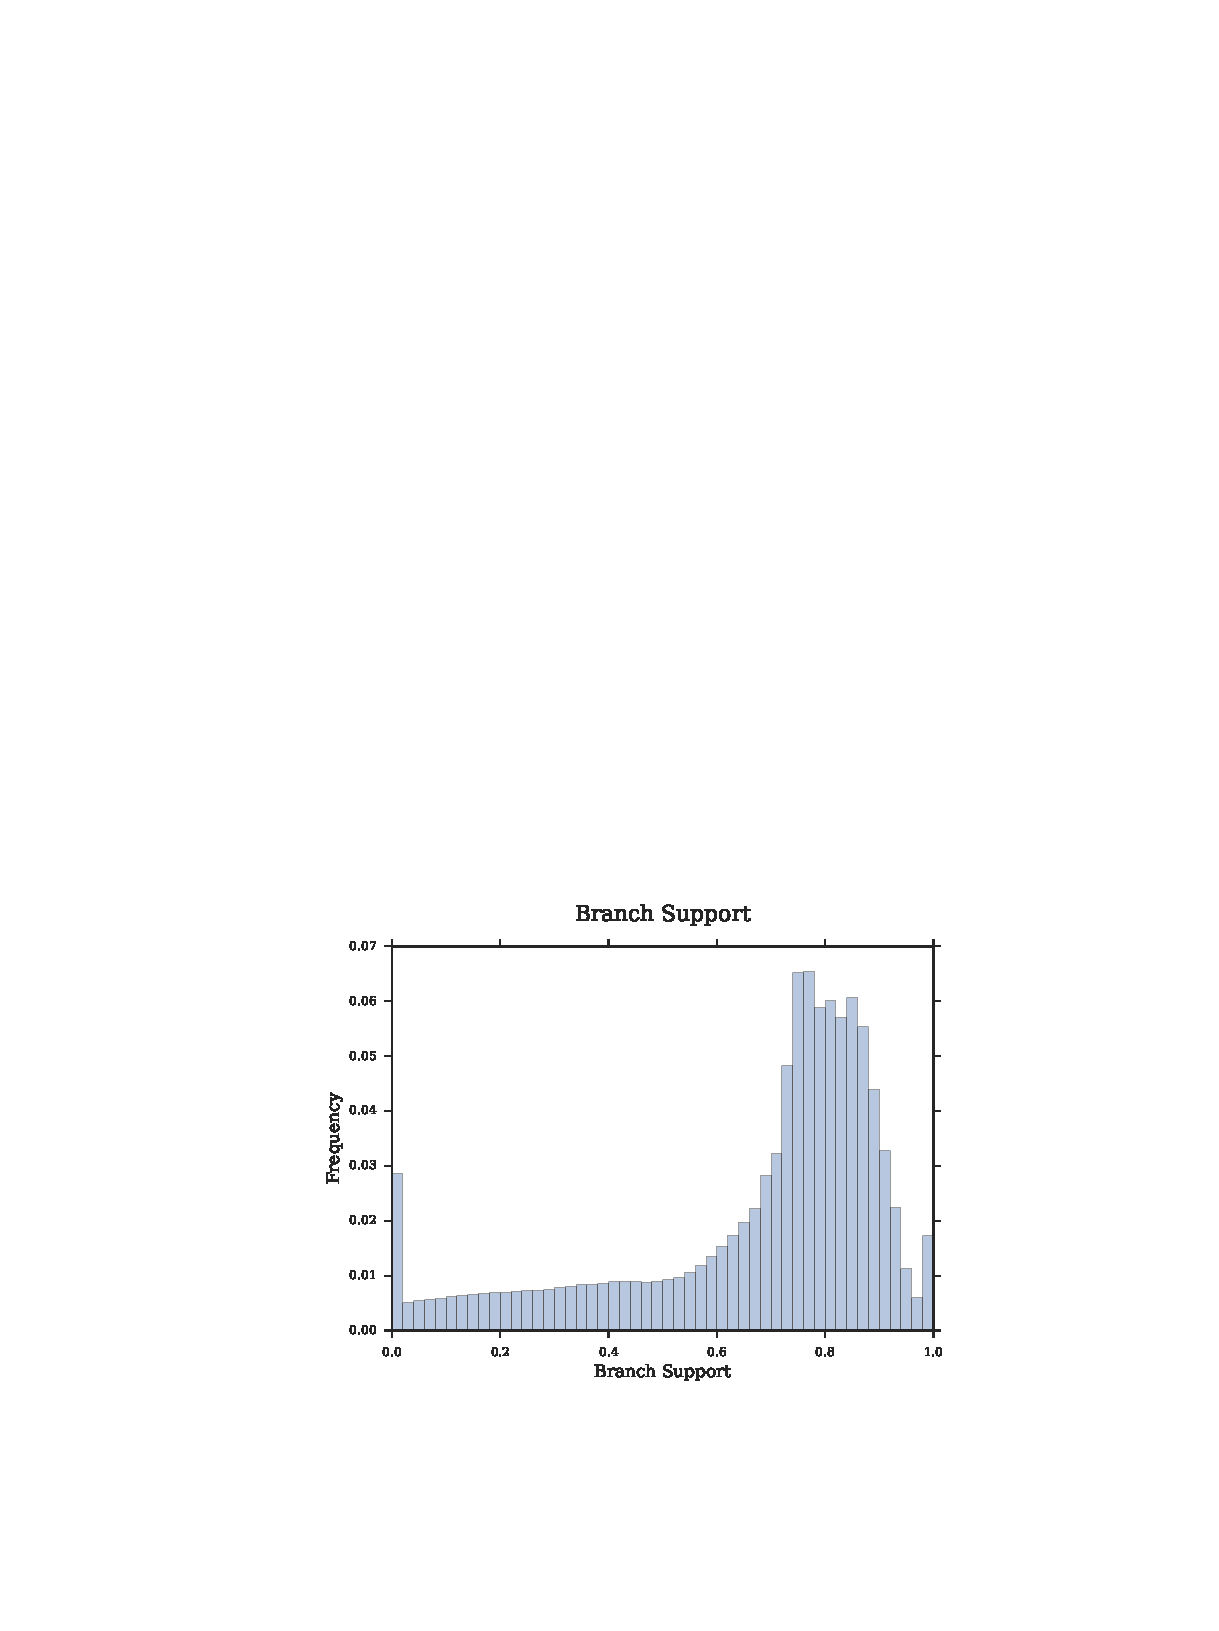
\includegraphics[width=0.8\textwidth]{figs/dualbirth-support-vals}
\caption[Human \textit{Alu} tree branch support]
{Human \textit{ Alu} tree branch support. Histogram of SH-like branch support values in the tree constructed from the masked alignment using FastTree~2. As can be seen, there are many low-support branches. Values below 0.9 are typically considered low SH-like support.}
\label{fig:dualbirth-support-vals}
\end{figure}

\begin{figure} % FIGURE S8 IN ORIGINAL PAPER
\centering
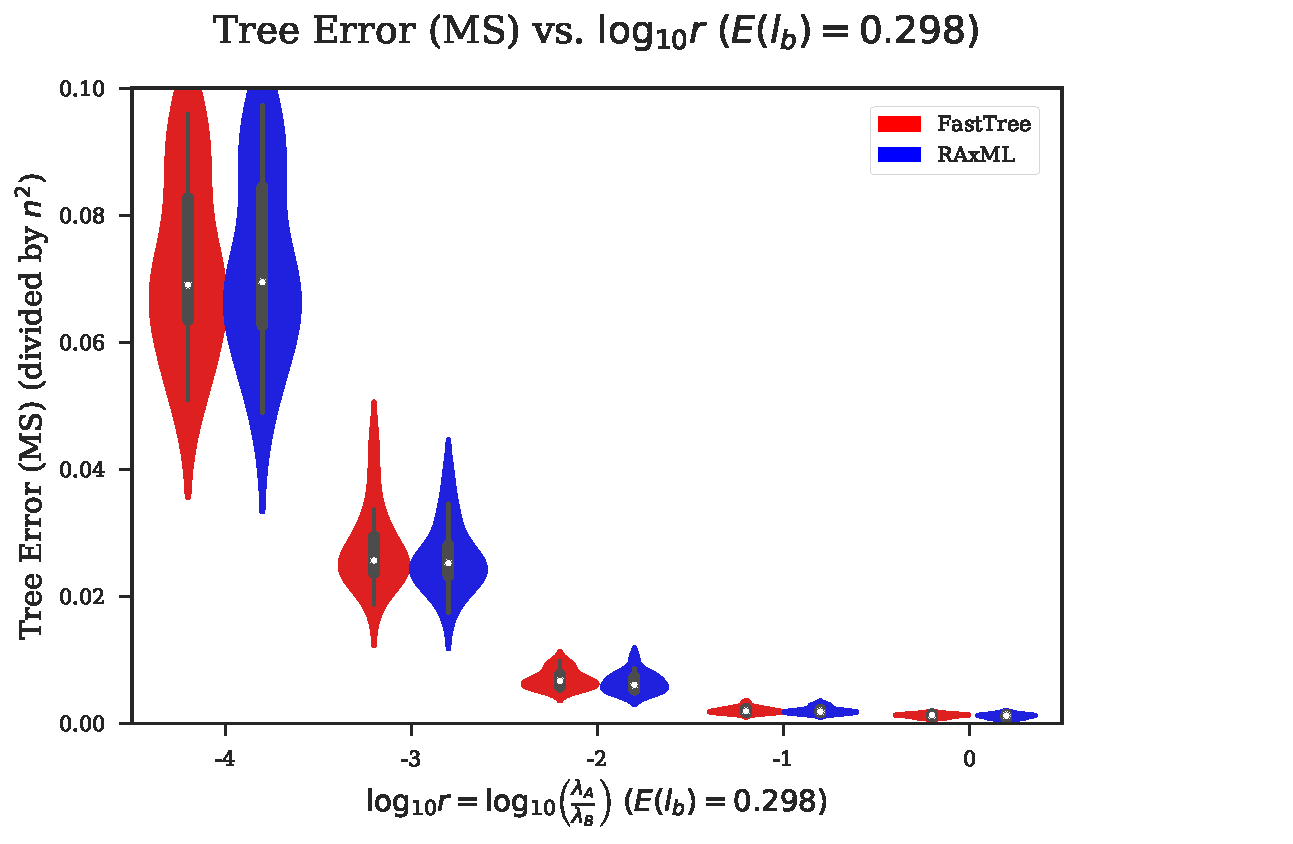
\includegraphics[width=0.3\textwidth]{figs/dualbirth-tree-ms-a}
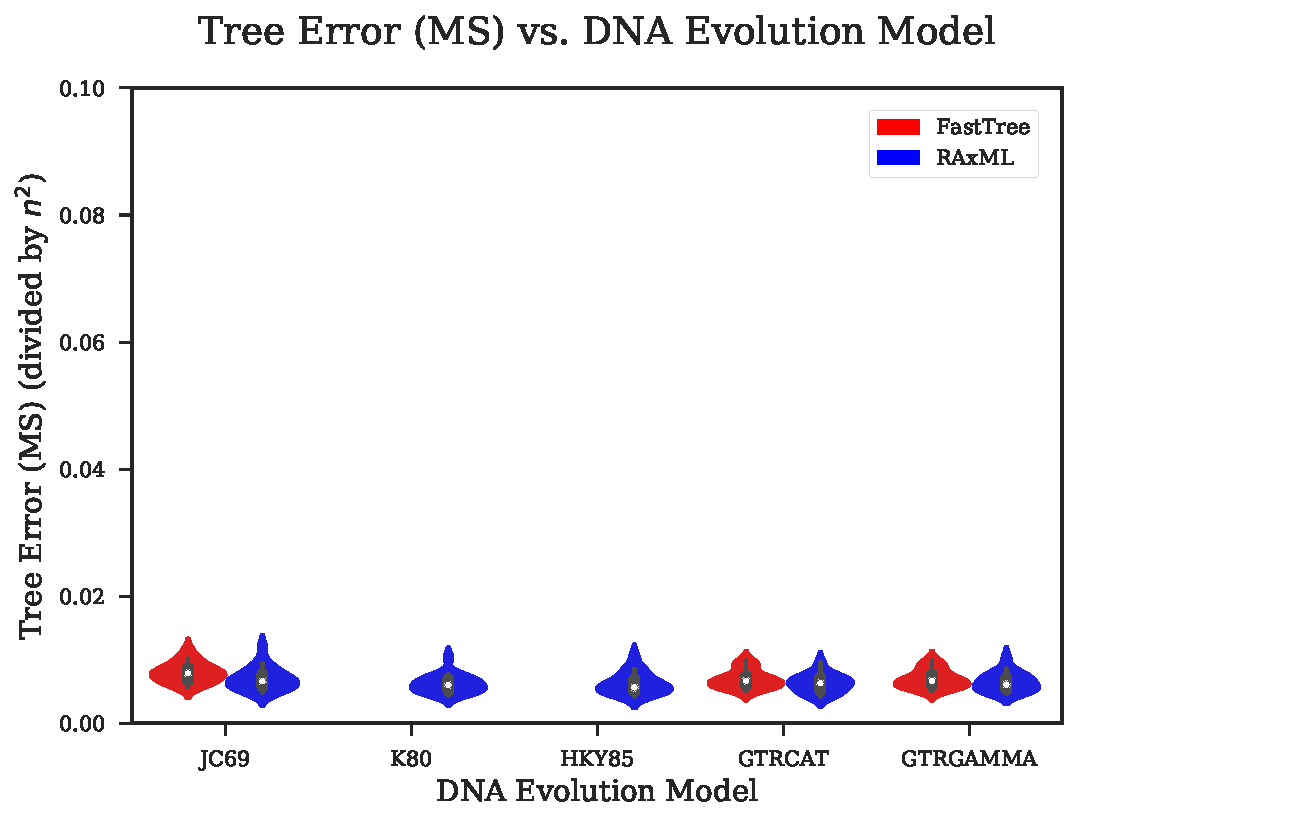
\includegraphics[width=0.3\textwidth]{figs/dualbirth-tree-ms-b}
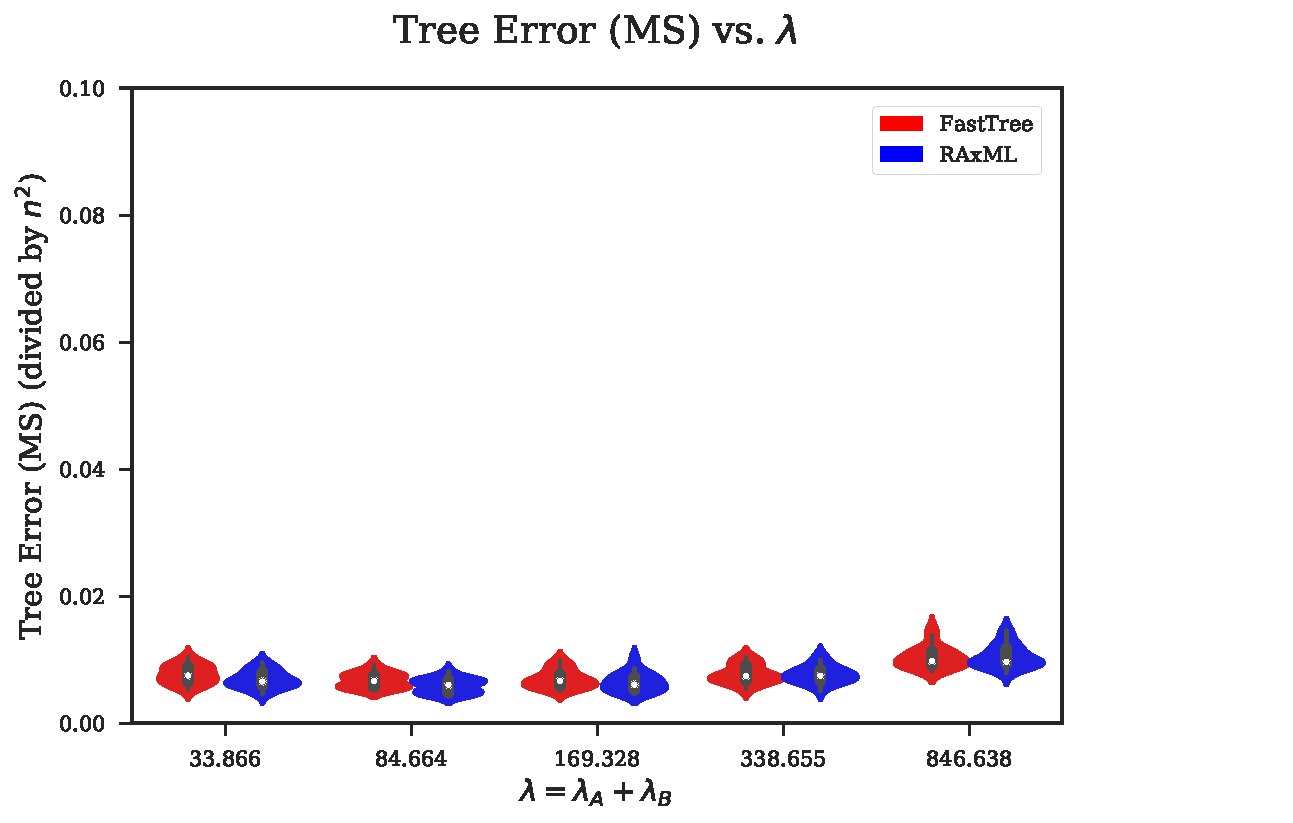
\includegraphics[width=0.3\textwidth]{figs/dualbirth-tree-ms-c}\\
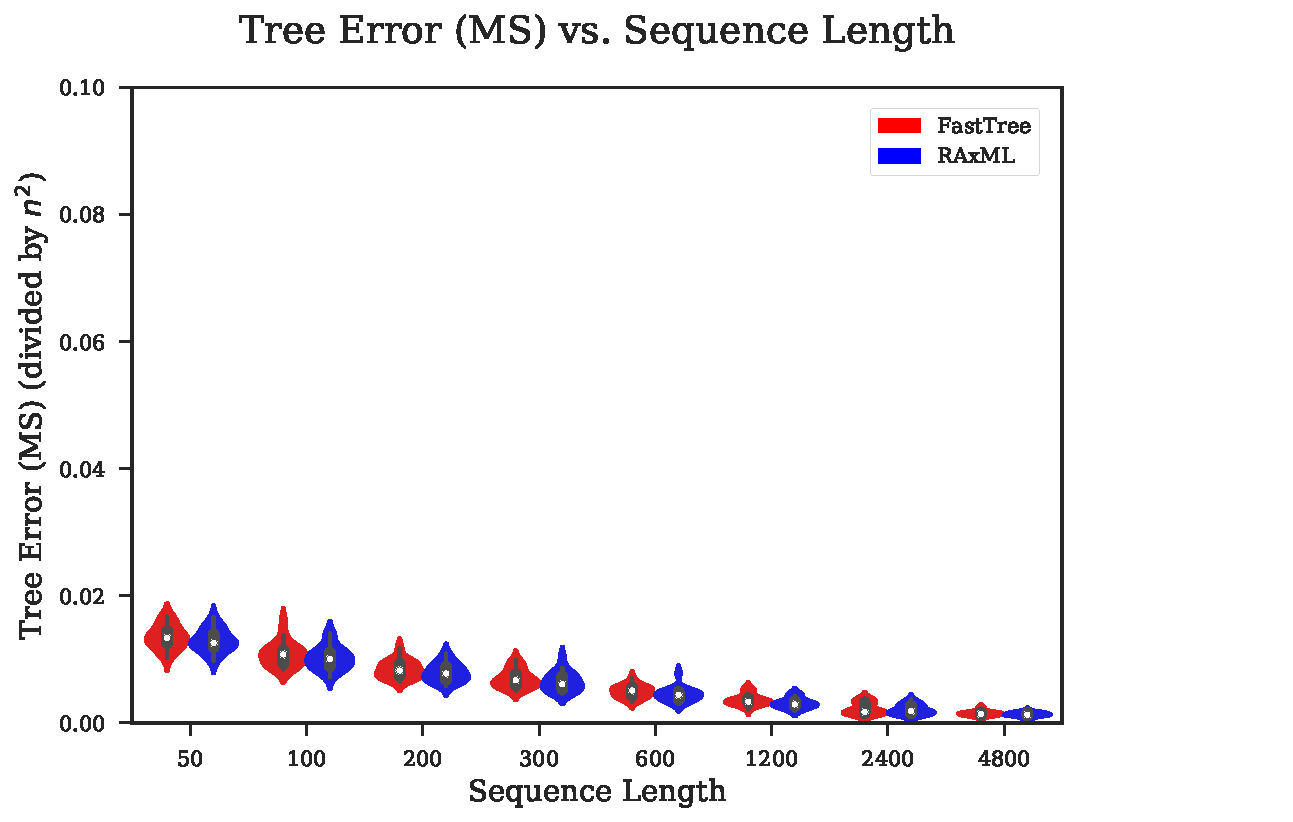
\includegraphics[width=0.3\textwidth]{figs/dualbirth-tree-ms-d}
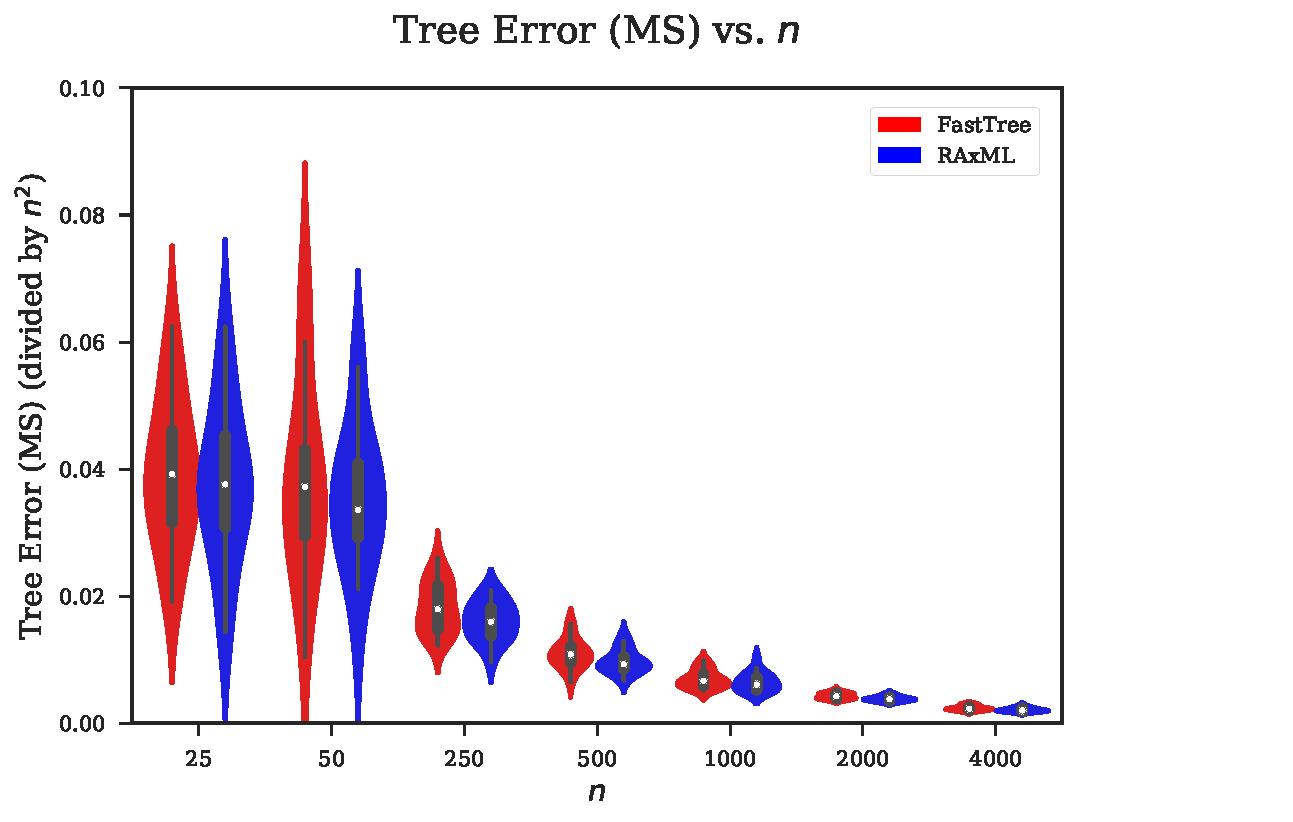
\includegraphics[width=0.3\textwidth]{figs/dualbirth-tree-ms-e}
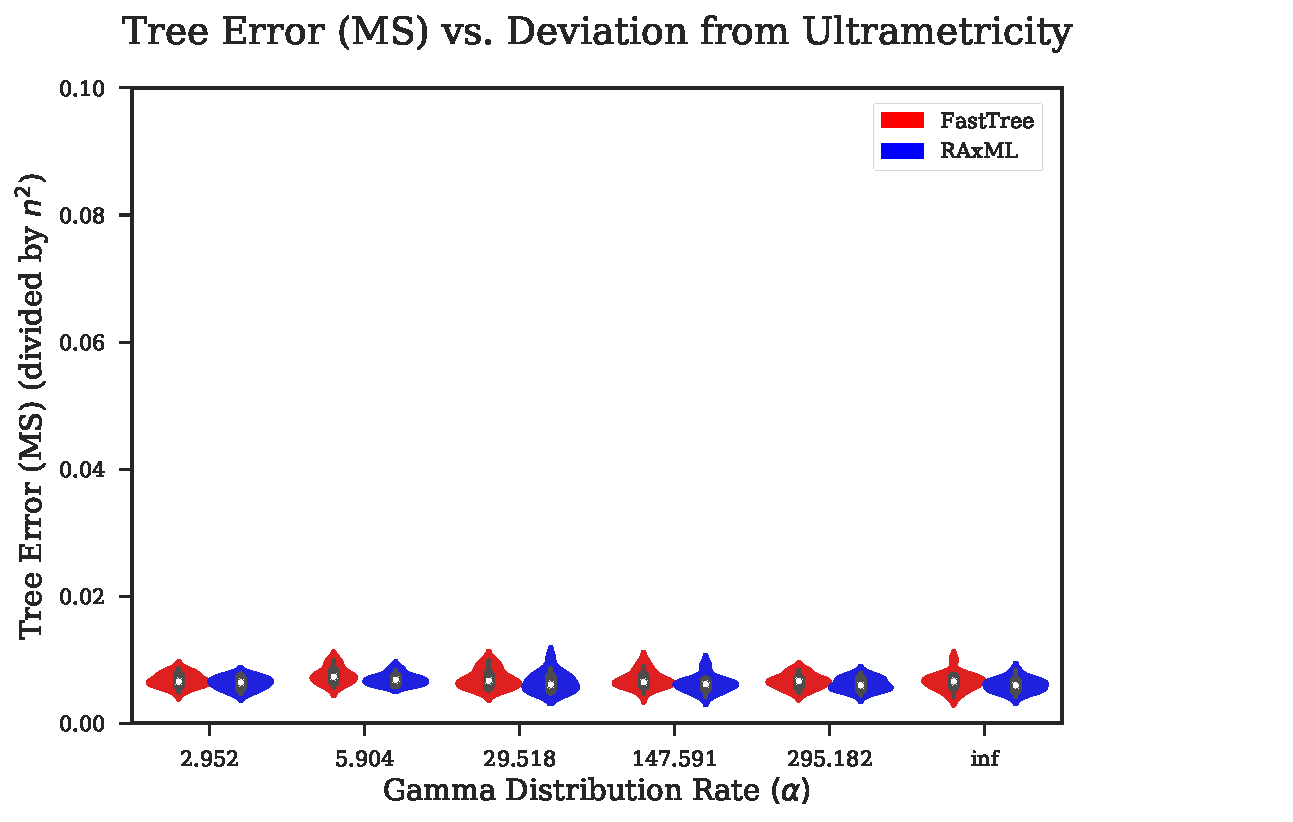
\includegraphics[width=0.3\textwidth]{figs/dualbirth-tree-ms-f}
\caption[Tree inference error (MS)]
{Tree inference error (MS). Violin plots are shown for the MS distance between true and estimated trees.}
\label{fig:dualbirth-tree-ms}
\end{figure}

\begin{figure} % FIGURE S9 IN ORIGINAL PAPER
\centering
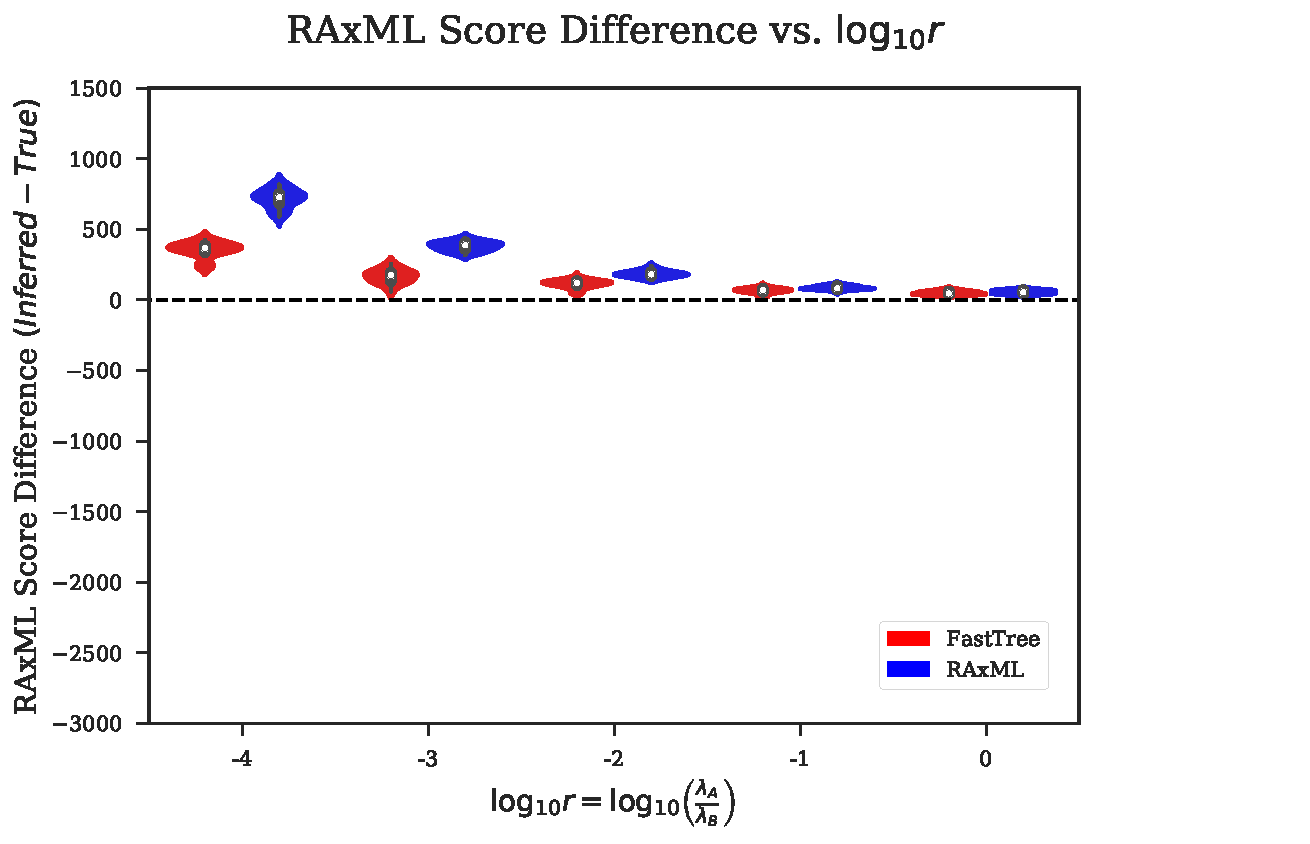
\includegraphics[width=0.3\textwidth]{figs/dualbirth-tree-score-diff-a}
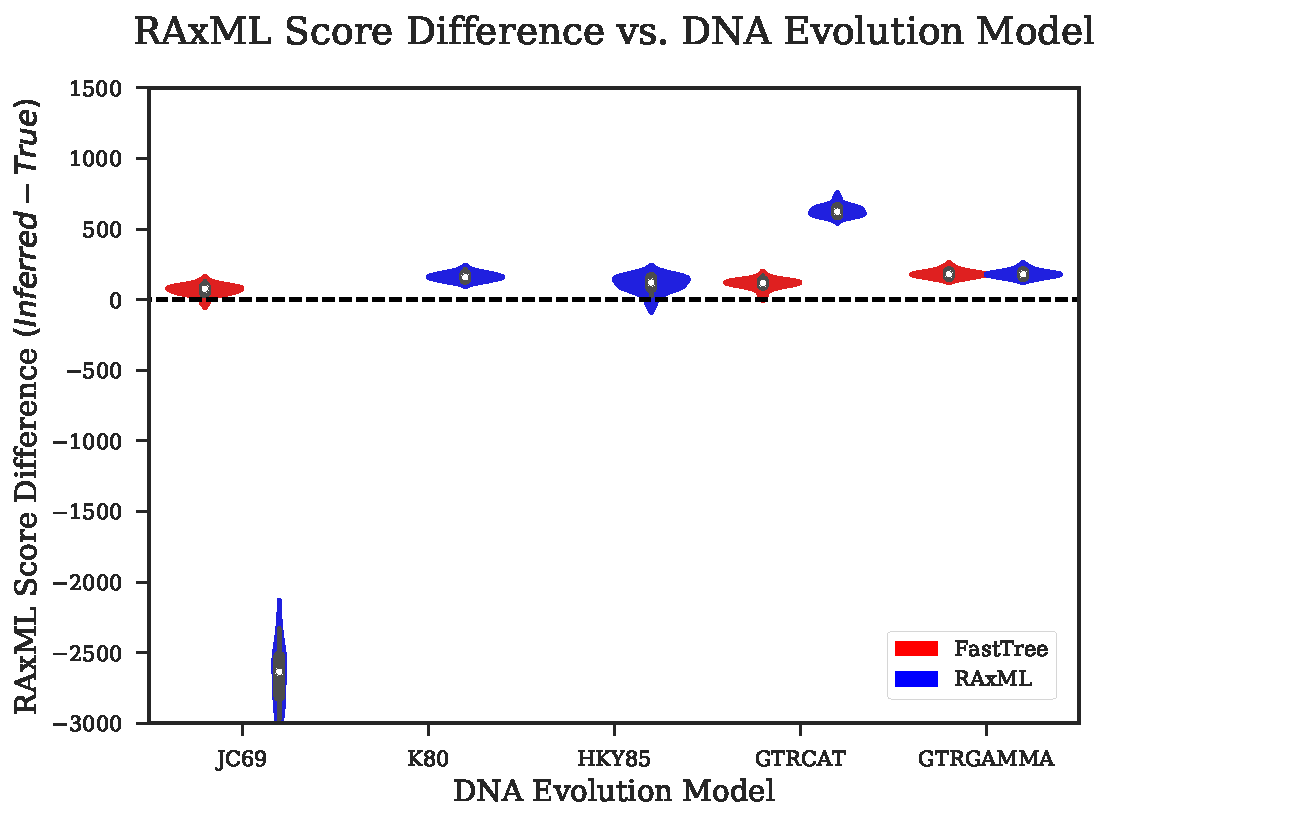
\includegraphics[width=0.3\textwidth]{figs/dualbirth-tree-score-diff-b}
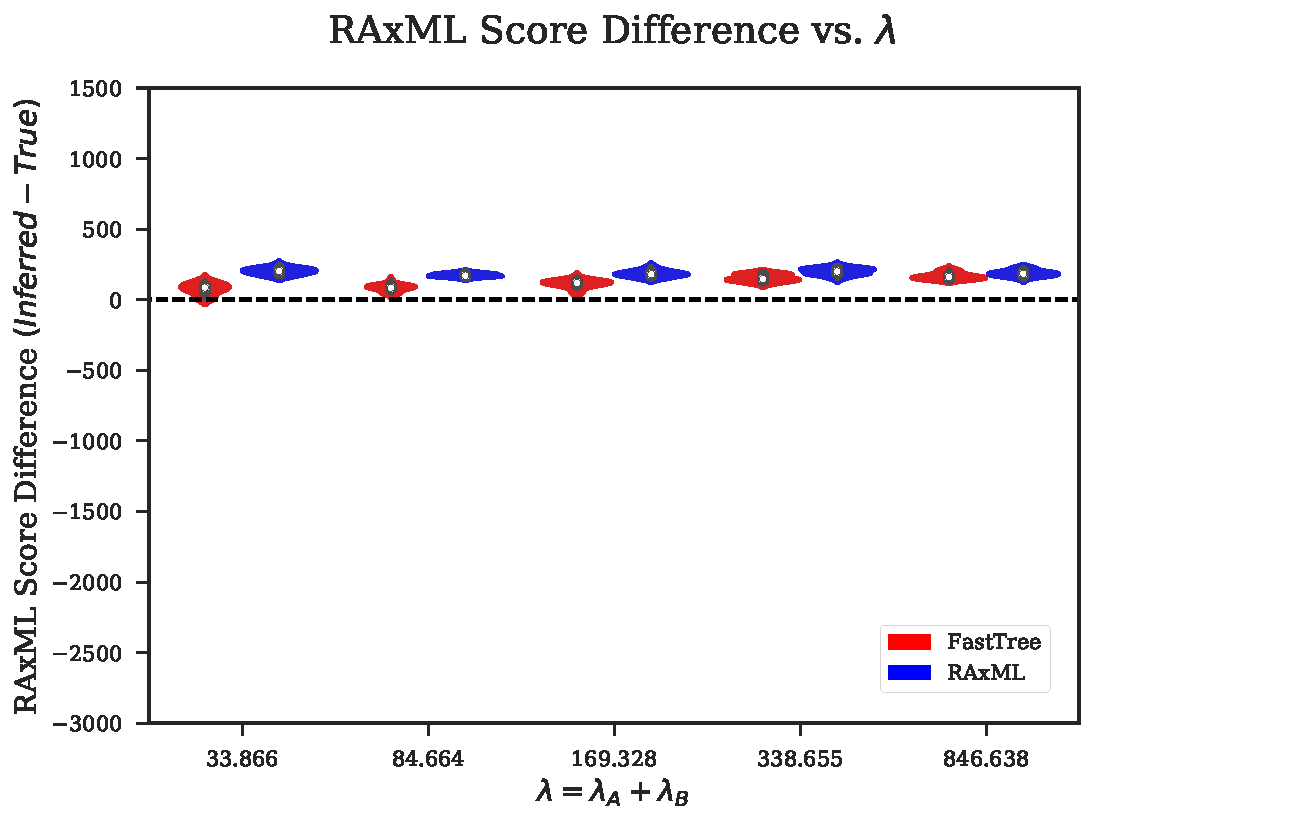
\includegraphics[width=0.3\textwidth]{figs/dualbirth-tree-score-diff-c}\\
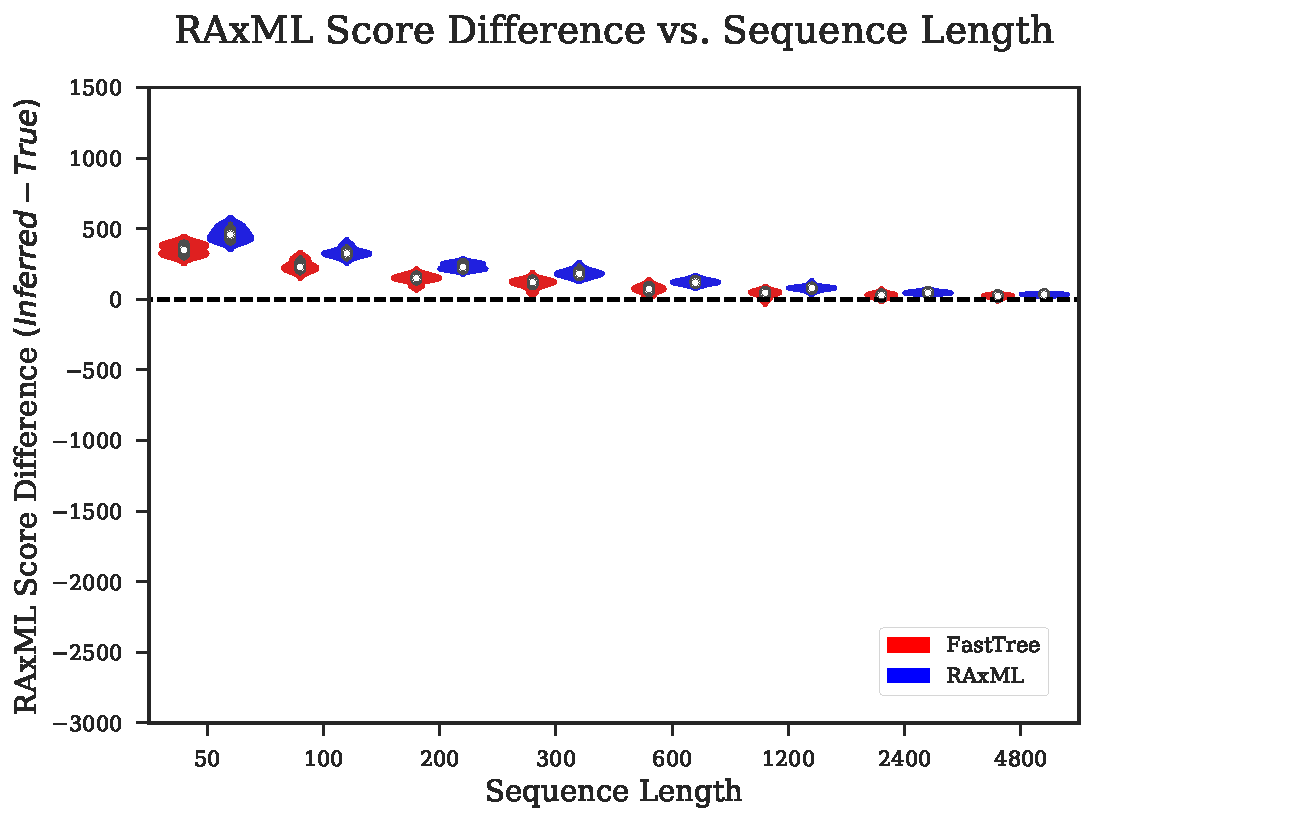
\includegraphics[width=0.3\textwidth]{figs/dualbirth-tree-score-diff-d}
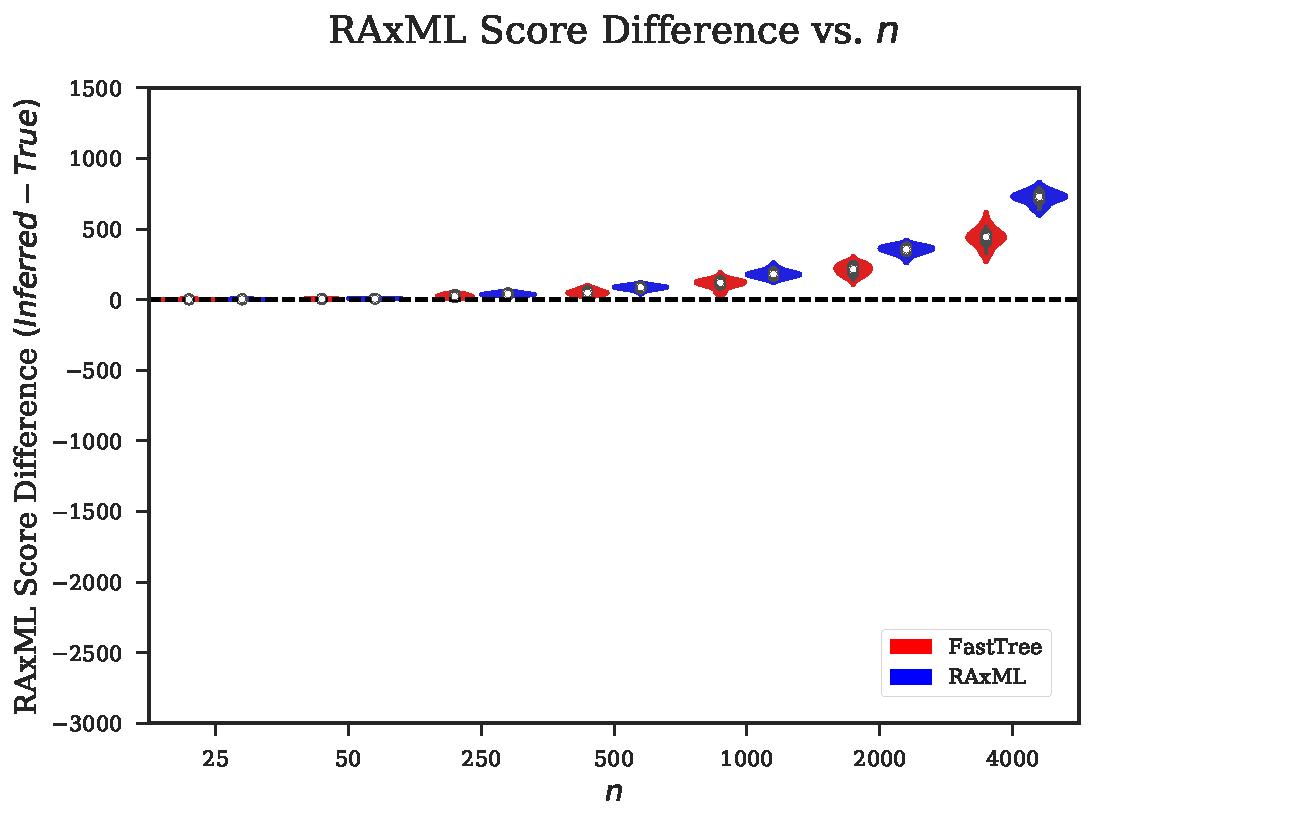
\includegraphics[width=0.3\textwidth]{figs/dualbirth-tree-score-diff-e}
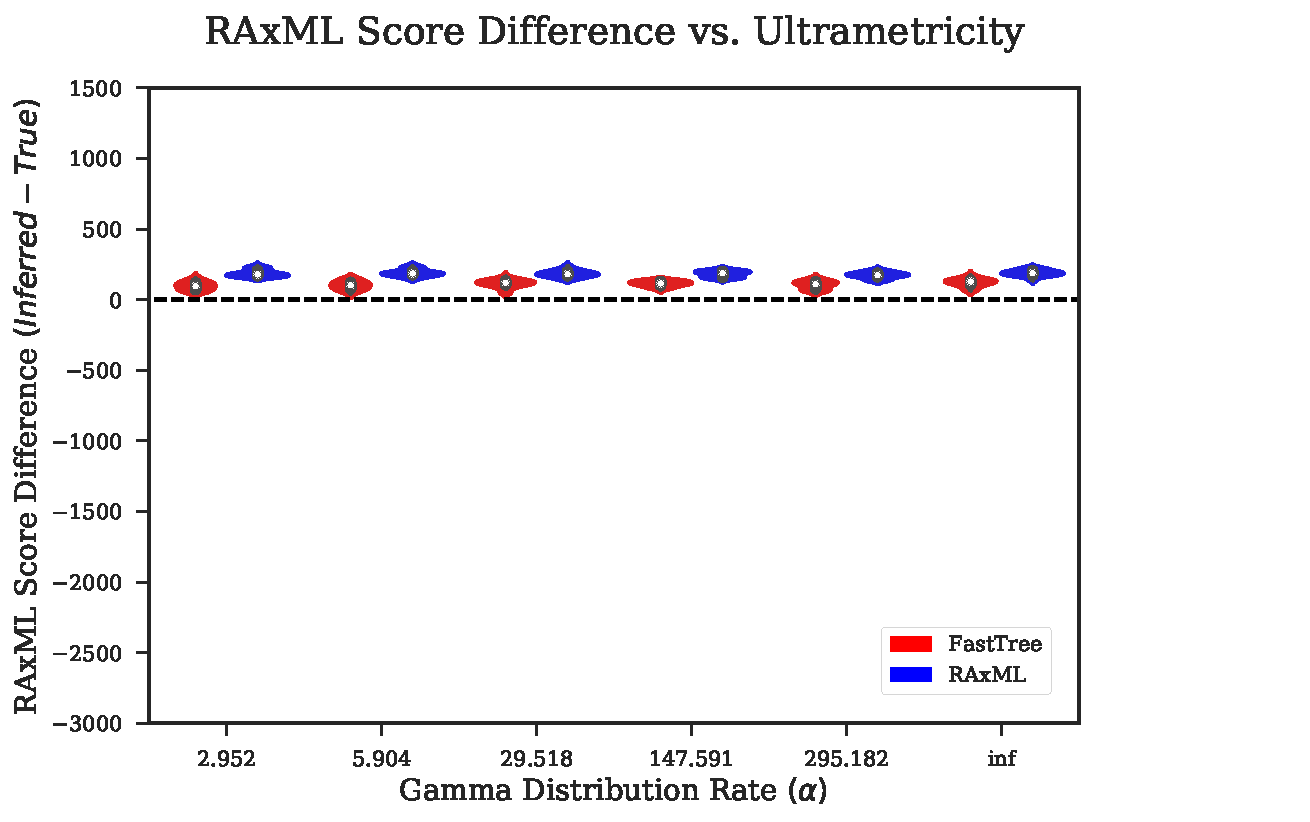
\includegraphics[width=0.3\textwidth]{figs/dualbirth-tree-score-diff-f}
\caption[Tree inference error]
{Tree inference error. Violin plots are shown for the log-likelihood score, as computed by RAxML, of the inferred tree minus the true tree; values away from zero indicate that the true tree has low log-likelihood scores.}
\label{fig:dualbirth-tree-score-diff}
\end{figure}

\begin{figure} % FIGURE S10 IN ORIGINAL PAPER
\centering
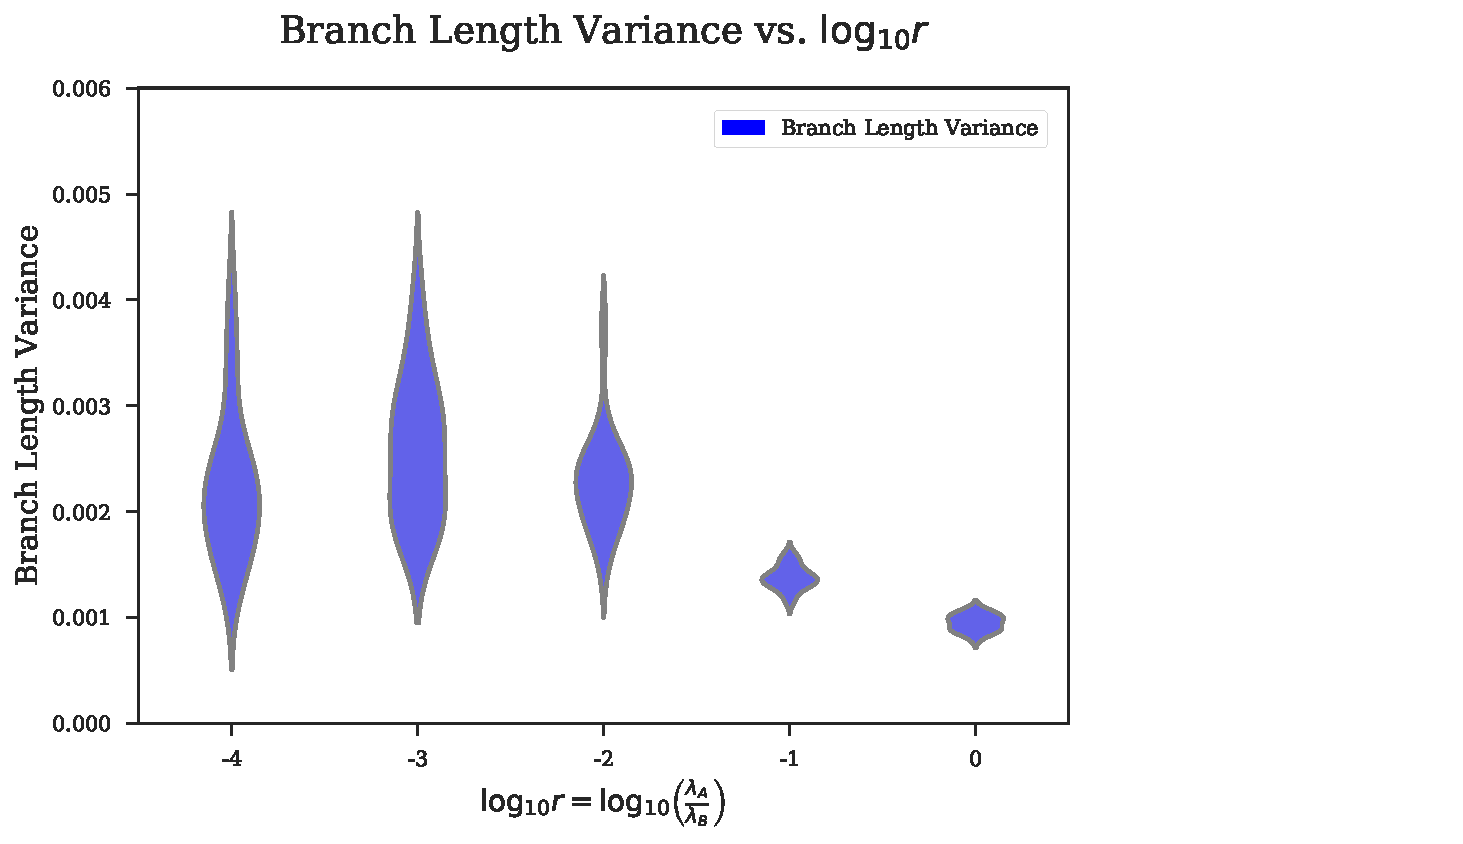
\includegraphics[width=0.3\textwidth]{figs/dualbirth-tree-bl-supp-a}
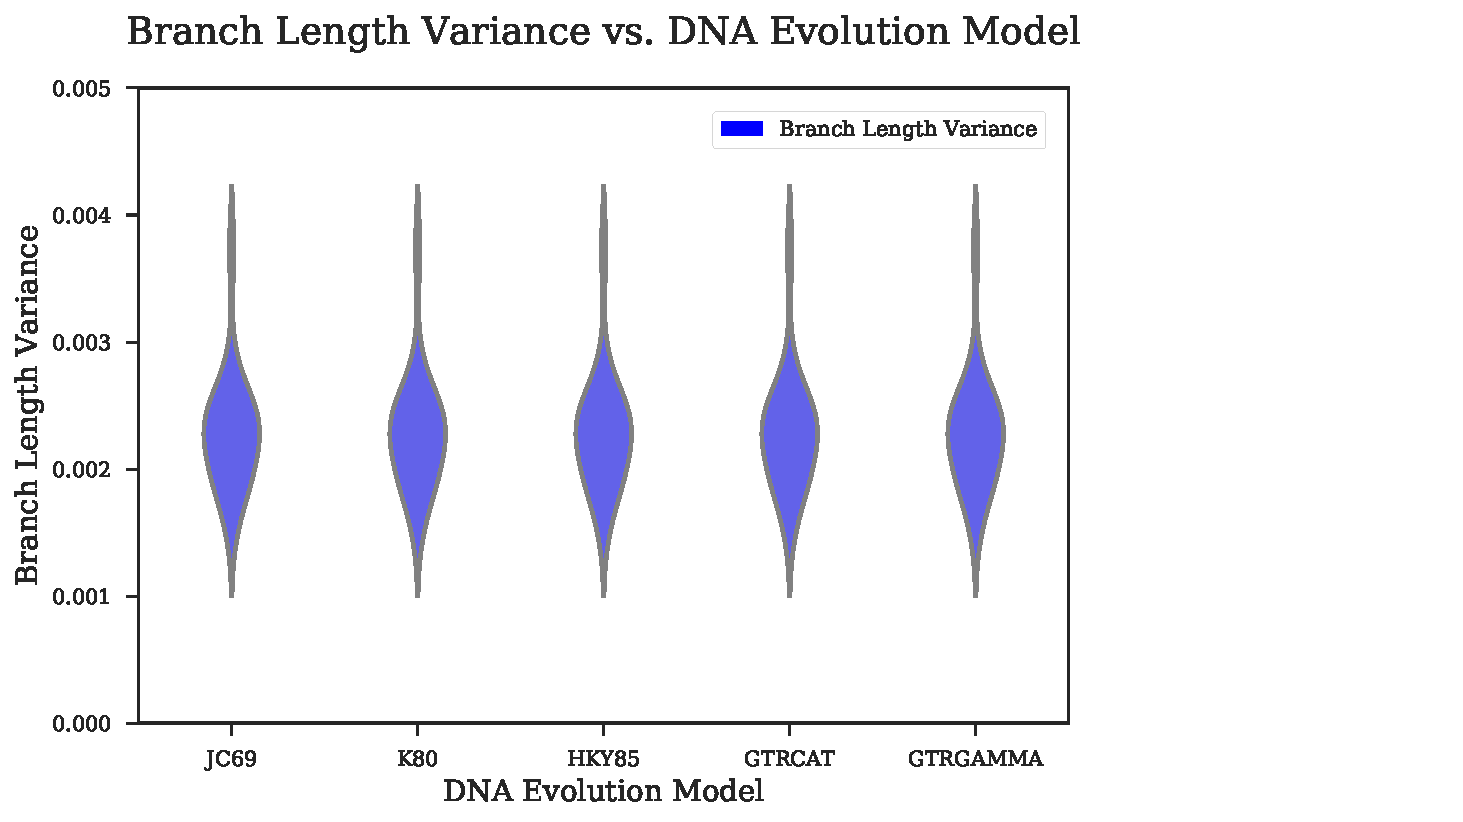
\includegraphics[width=0.3\textwidth]{figs/dualbirth-tree-bl-supp-b}
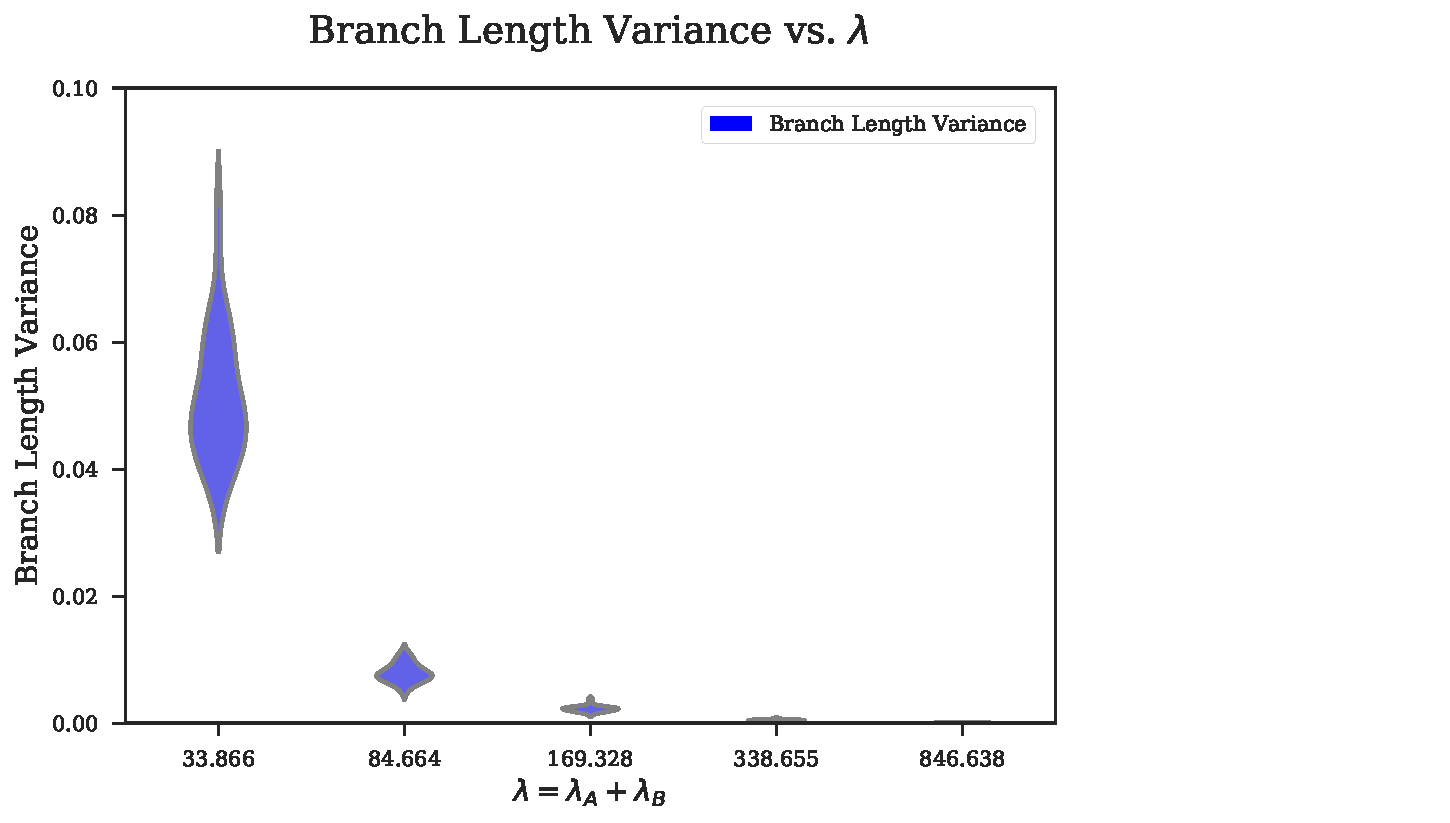
\includegraphics[width=0.3\textwidth]{figs/dualbirth-tree-bl-supp-c}\\
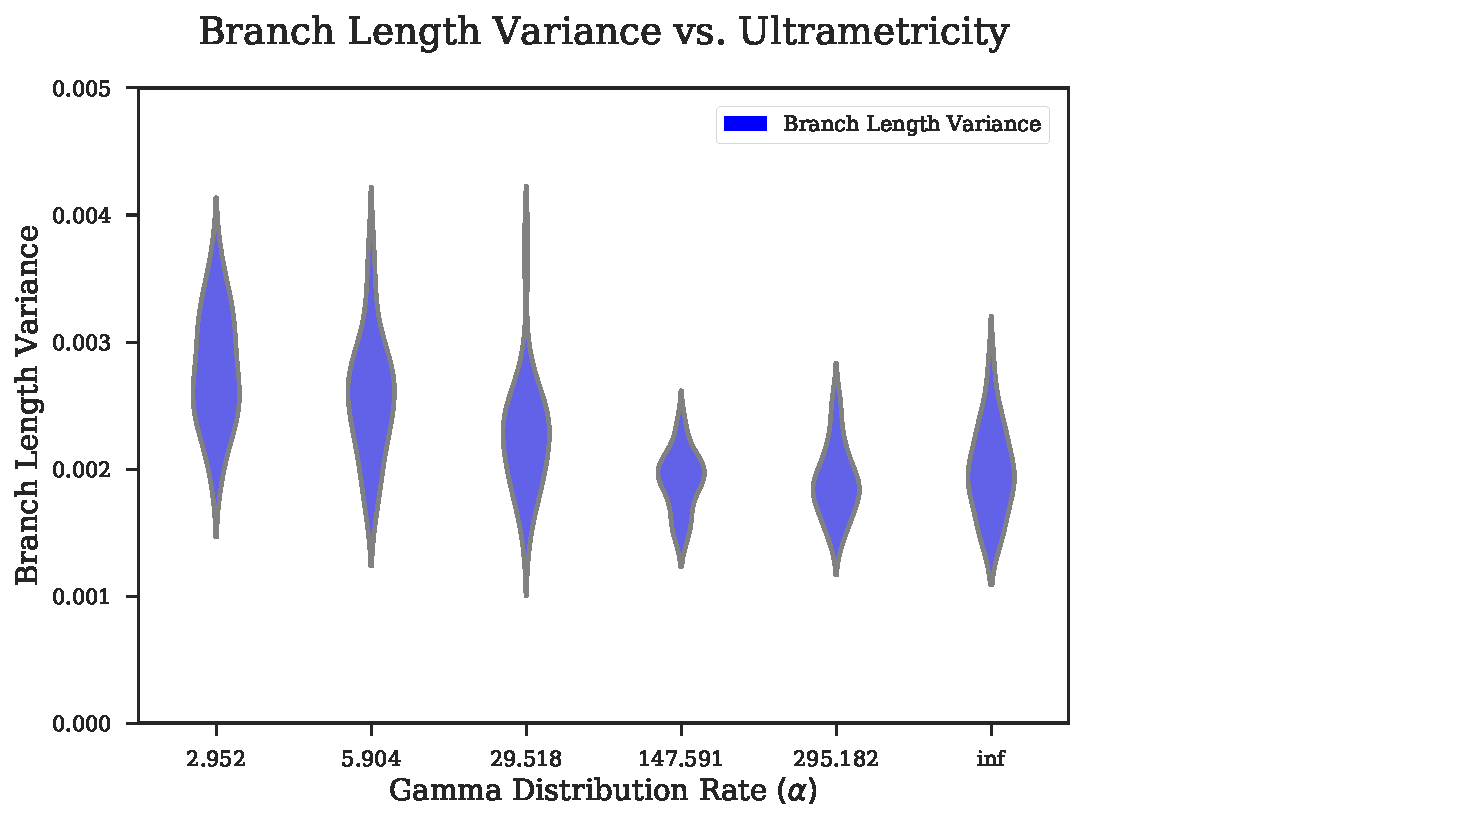
\includegraphics[width=0.3\textwidth]{figs/dualbirth-tree-bl-supp-d}
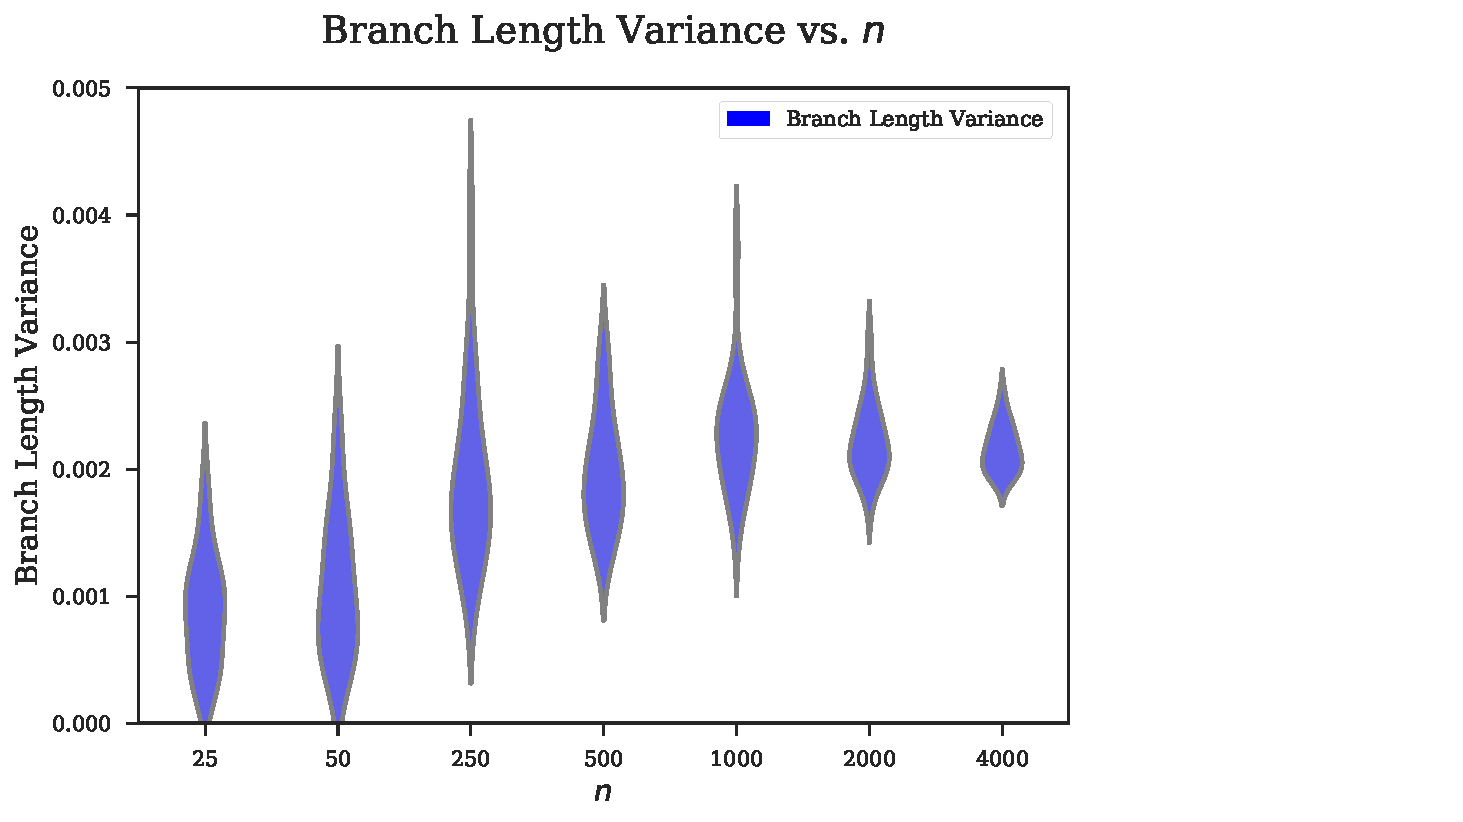
\includegraphics[width=0.3\textwidth]{figs/dualbirth-tree-bl-supp-e}
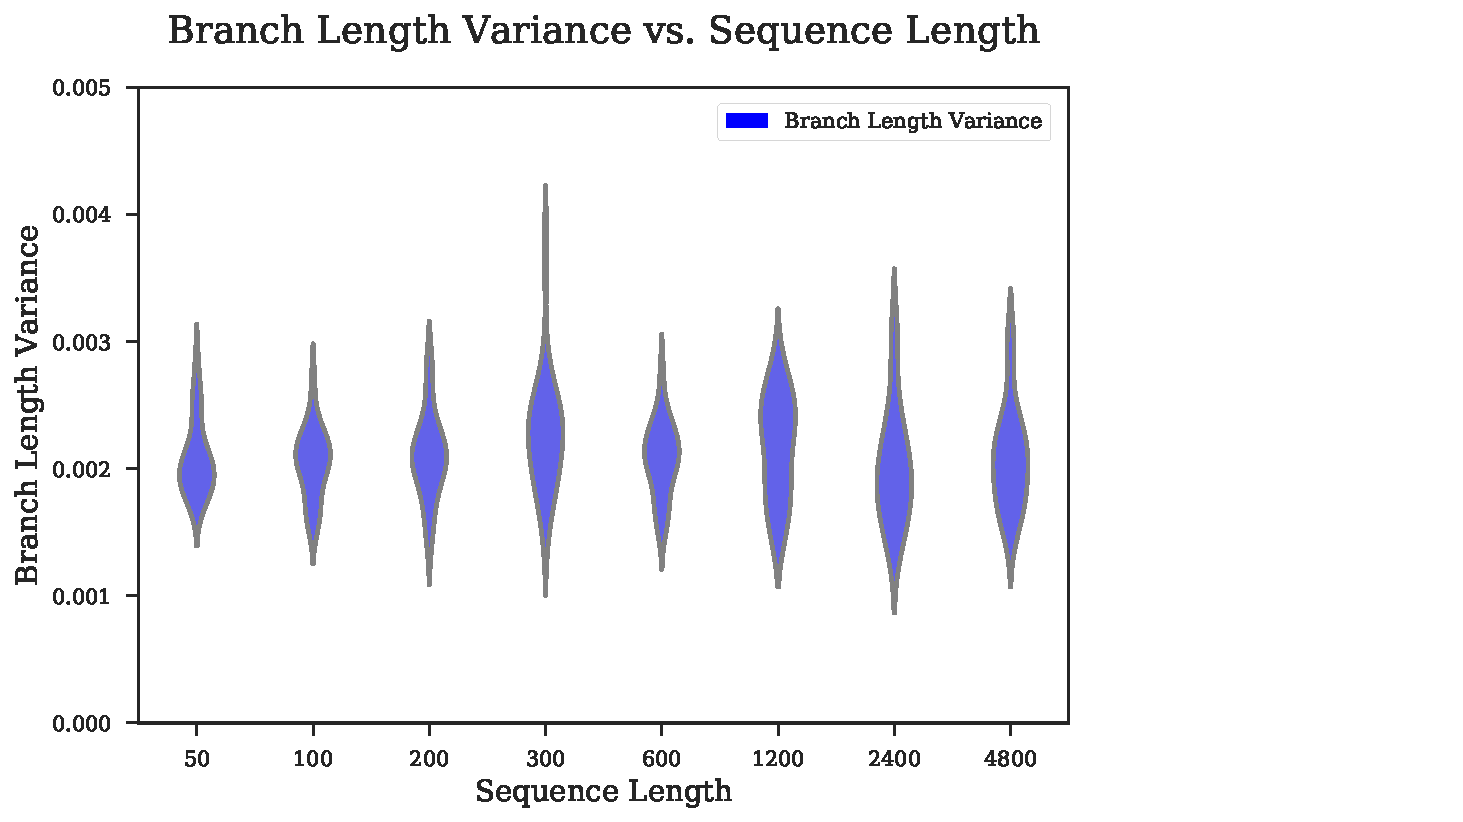
\includegraphics[width=0.3\textwidth]{figs/dualbirth-tree-bl-supp-f}
\caption[Branch length summary statistics]
{Branch length summary statistics. Violin plots are shown for the branch length variance computed for true trees.}
\label{fig:dualbirth-tree-bl-supp}
\end{figure}

\begin{figure} % FIGURE S11 IN ORIGINAL PAPER
\centering
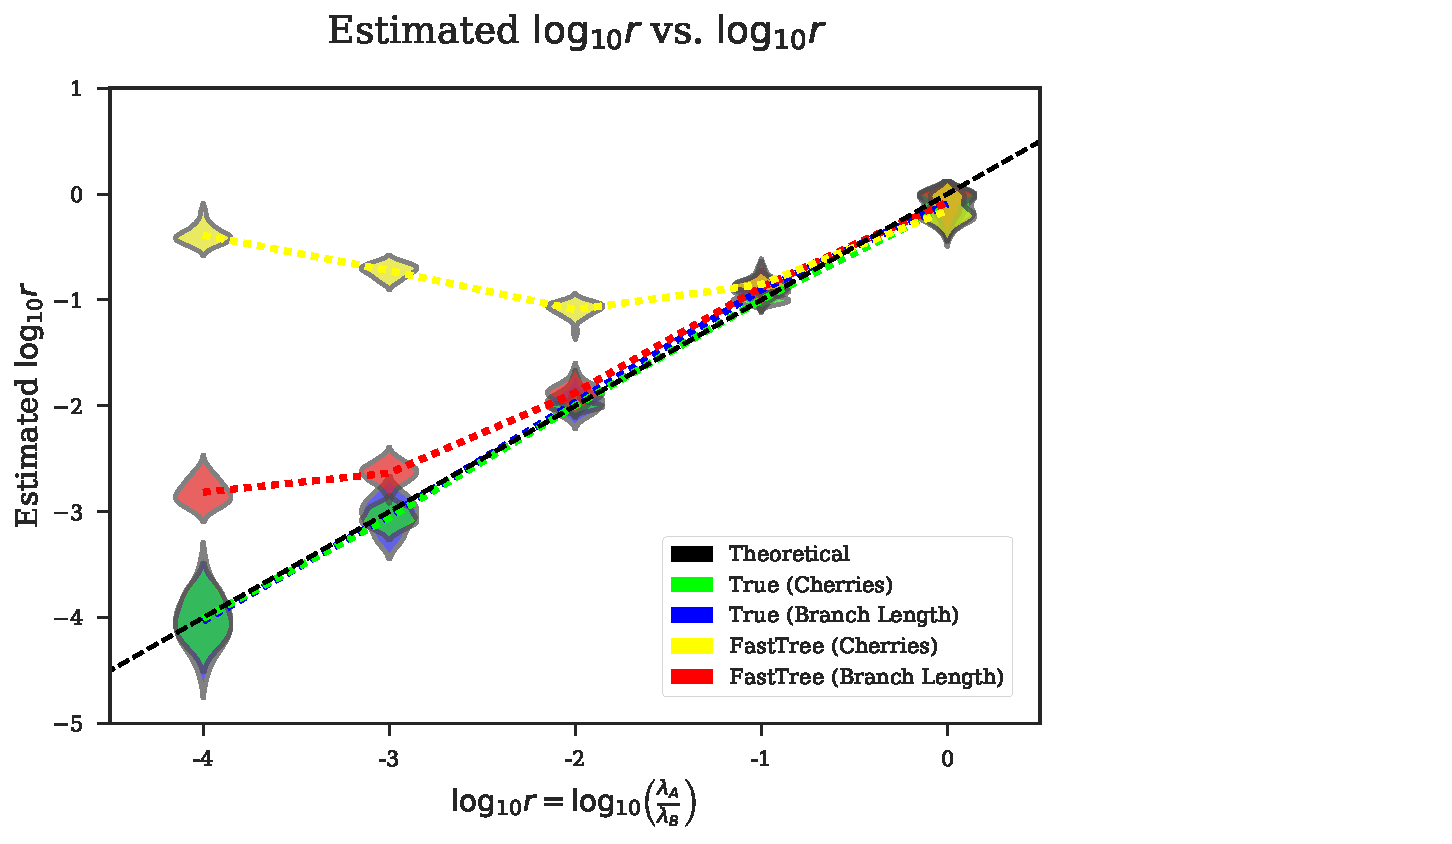
\includegraphics[width=0.3\textwidth]{figs/dualbirth-res-cherry-supp-a}
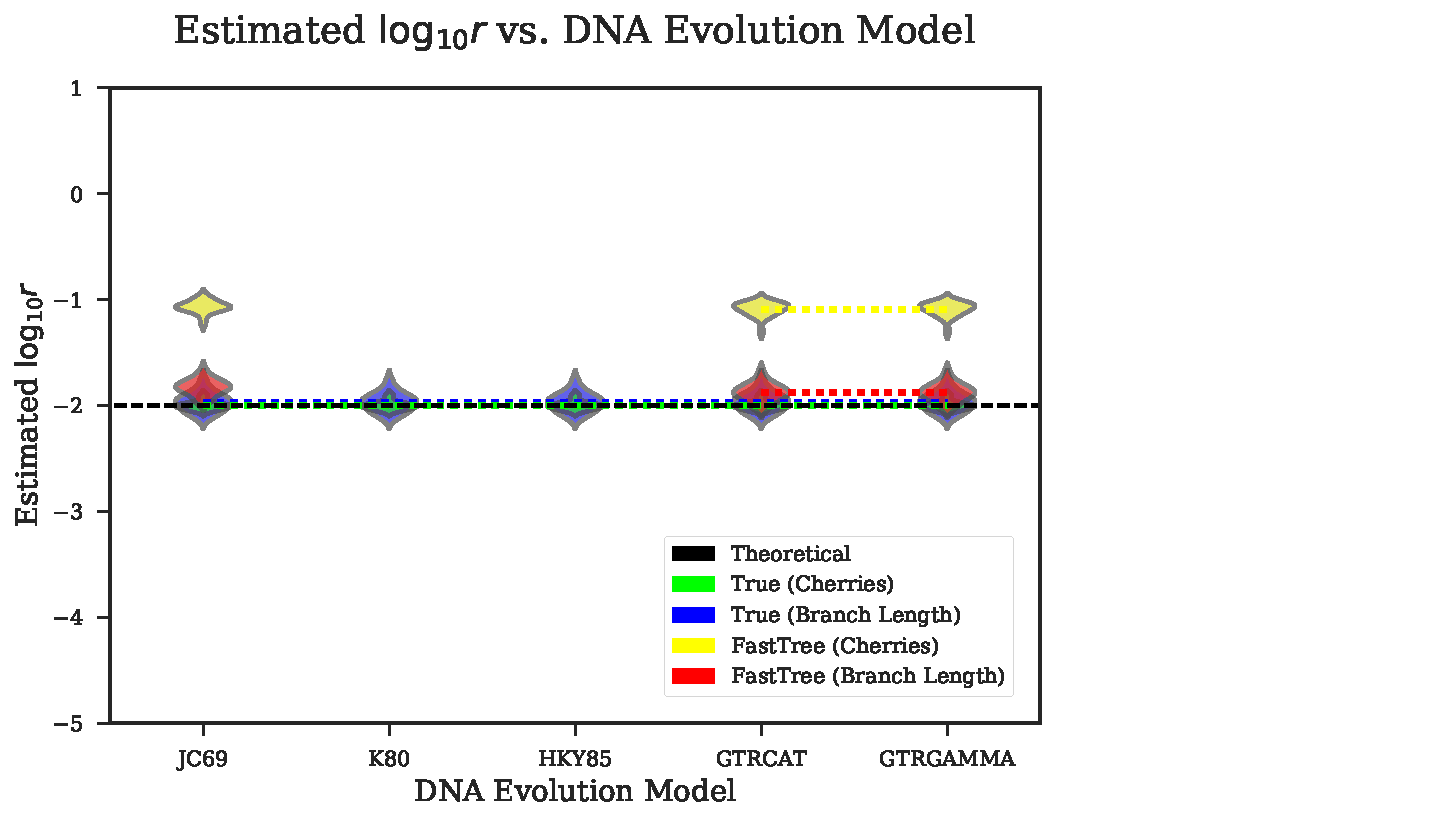
\includegraphics[width=0.3\textwidth]{figs/dualbirth-res-cherry-supp-b}
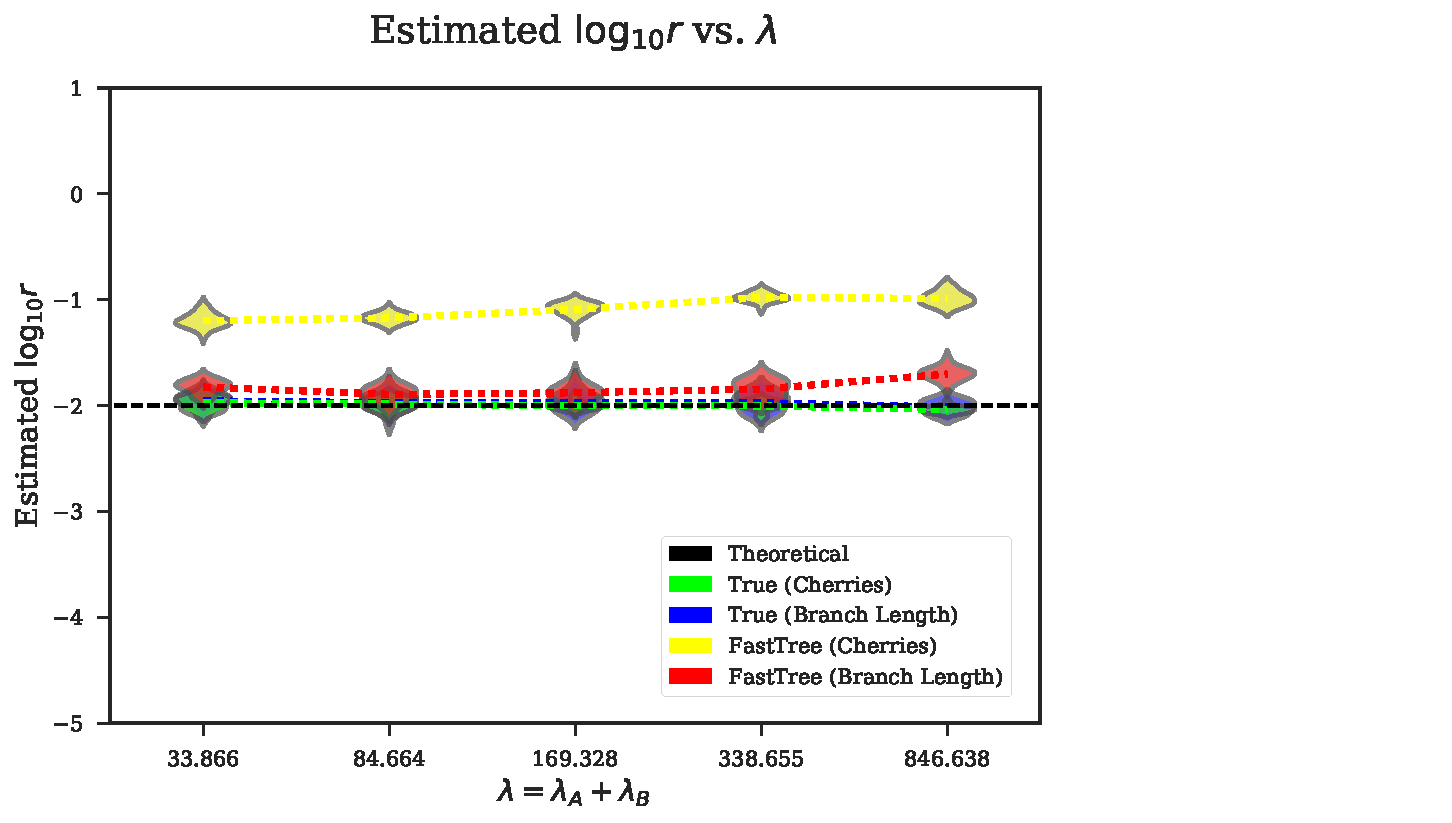
\includegraphics[width=0.3\textwidth]{figs/dualbirth-res-cherry-supp-c}\\
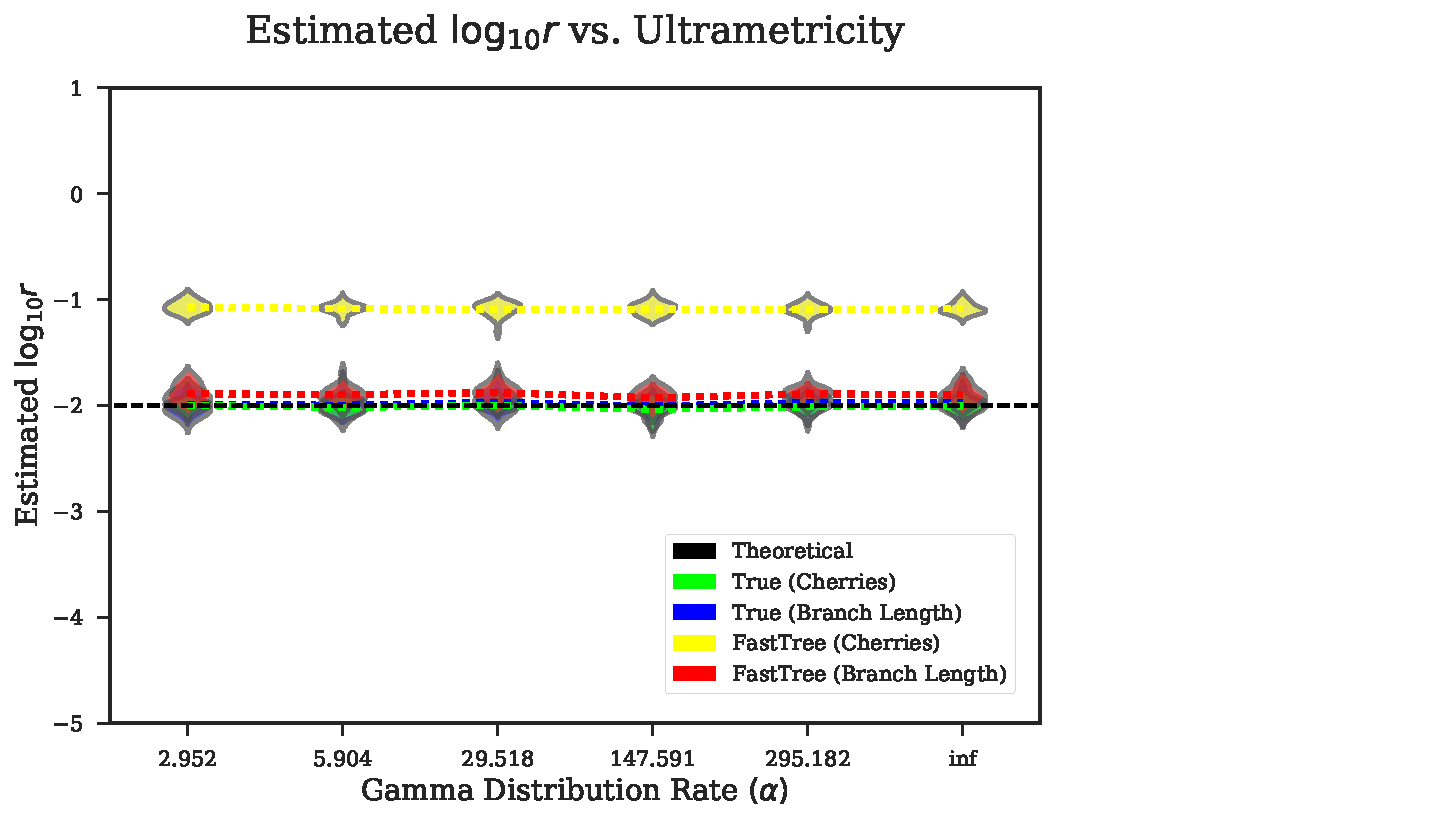
\includegraphics[width=0.3\textwidth]{figs/dualbirth-res-cherry-supp-d}
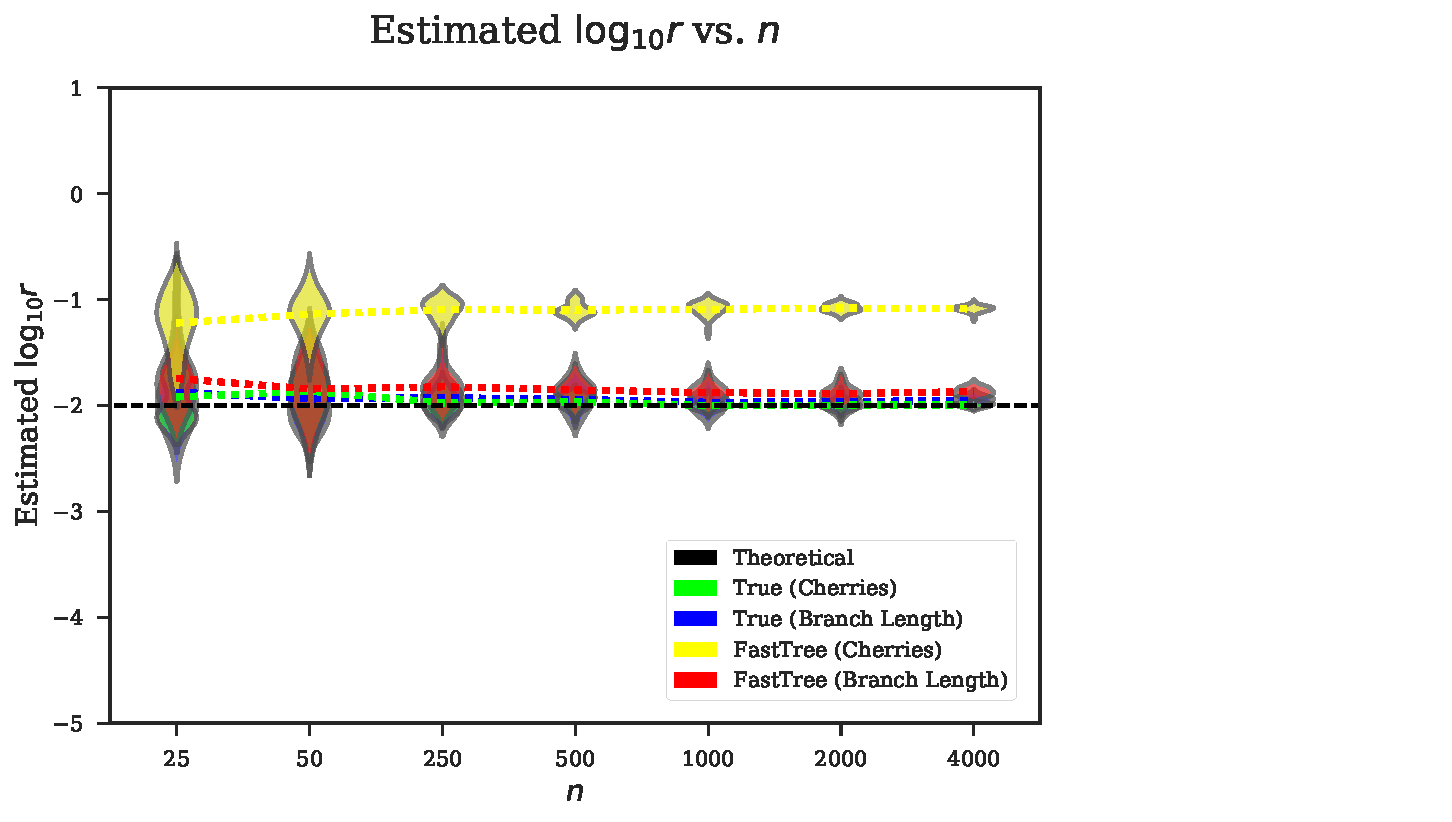
\includegraphics[width=0.3\textwidth]{figs/dualbirth-res-cherry-supp-e}
\includegraphics[width=0.3\textwidth]{figs/dualbirth-res-cherry-supp-f}
\caption[Parameter estimation accuracy]
{Parameter estimation accuracy. Violin plots are shown for the estimated $r$, using the cherry-based estimator and the branch-length-based estimator, for true trees and for inferred FastTree~2 trees for each of the experiments. Note that FastTree~2 does not have \gls{K80} or \gls{HKY85} models implemented.}
\label{fig:dualbirth-res-cherry-supp}
\end{figure}

\begin{figure} % FIGURE S12 IN ORIGINAL PAPER
\centering
\includegraphics[width=0.3\textwidth]{figs/dualbirth-cherry-fraction-supp-a}
\includegraphics[width=0.3\textwidth]{figs/dualbirth-cherry-fraction-supp-b}
\includegraphics[width=0.3\textwidth]{figs/dualbirth-cherry-fraction-supp-c}\\
\includegraphics[width=0.3\textwidth]{figs/dualbirth-cherry-fraction-supp-d}
\includegraphics[width=0.3\textwidth]{figs/dualbirth-cherry-fraction-supp-e}
\includegraphics[width=0.3\textwidth]{figs/dualbirth-cherry-fraction-supp-f}
\caption[Cherry fraction]
{Cherry fraction. Violin plots are shown for the cherry fractions of the true trees and inferred RAxML and FastTree~2 trees.}
\label{fig:dualbirth-cherry-fraction-supp}
\end{figure}

\begin{figure} % FIGURE S13 IN ORIGINAL PAPER
\centering
\includegraphics[width=0.8\textwidth]{figs/dualbirth-root-to-tip}
\caption[Molecular clock on the \textit{ Alu} tree]
{Molecular clock on the \textit{ Alu} tree. The distribution of the root-to-tip distances after midpoint rooting are shown for the \textit{ Alu} tree with 1\% masking. Under the molecular clock, root to tip distances for all leaves are expected to be identical.}
\label{fig:dualbirth-root-to-tip}
\end{figure}

%% END DUAL-BIRTH SUPPLEMENT
%% START PROACT SUPPLEMENT
\chapter{Supplemental Material for Chapter~\ref{chap:proact}}
\label{chap:proact-sup}
\clearpage

%% END PROACT SUPPLEMENT
%%% START TREESWIFT SUPPLEMENT
\chapter{Supplemental Material for Chapter~\ref{chap:treeswift}}
\label{chap:treeswift-sup}
\clearpage

%% END TREESWIFT SUPPLEMENT
%%% START EDUCATION SUPPLEMENT
\chapter{Supplemental Material for Chapter~\ref{chap:education}}
\label{chap:education-sup}
\clearpage

%% END EDUCATION SUPPLEMENT

%% End Matter
% \printindex %% Uncomment to display the index
\bibliographystyle{ieeetr}
\bibliography{dissertation}
\singlespace

\end{document}